The \tHq\ signal is separated from the main backgrounds using a boosted decision tree (BDT) classifier, trained on simulated signal and background events.
A set of discriminating variables are given as input to the BDT which produces a output distribution maximizing the discrimination power.
Table~\ref{tab:bdtinputs} lists the input variables used while Figures~\ref{fig:input_vars_3l} and~\ref{fig:input_vars_2lss} show their distributions for the relevant signal and background samples, for the three lepton and same-sign dilepton channels, respectively.
The same or equivalent input variables are found to be performing well for both three lepton and same-sign dilepton channels.

Two BDT classifiers are trained for the two main backgrounds expected in the analysis: events with prompt leptons from \ttW\ and \ttZ\ (also referred to as \ttV), and events with non-prompt leptons from \ttbar.
The datasets used in the training are the \tHq\ signal (see Tab.~\ref{tab:sigsamples}), and LO \MADGRAPH\ samples of \ttW\ and \ttZ, in an admixture proportional to their respective cross sections (see Tab.~\ref{tab:ttvlo_samples}).

\begin{table}[h!]
\centering
\begin{tabular}{lp{10cm}}
Variable name        & Description\\ \hline
nJet25               & Number of jets with $\pt>25\GeV$, $|\eta|<2.4$\\
MaxEtaJet25          & Maximum $|\eta|$ of any (non-CSV-loose) jet with $\pt>25\GeV$\\
% nBJetLoose25         & Number of jets with $\pt>25\GeV$, CSV loose\\
totCharge            & Sum of lepton charges \\
nJetEta1             & Number of jets with $|\eta|>1.0$, non-CSV-loose\\
detaFwdJetBJet       & $\Delta \eta$ between forward light jet and hardest CSV loose jet\\
detaFwdJet2BJet      & $\Delta \eta$ between forward light jet and second hardest CSV loose jet (defaults to -1 in events with only one CSV loose jet) \\
detaFwdJetClosestLep & $\Delta \eta$ between forward light jet and closest lepton\\
dphiHighestPtSSPair  & $\Delta \phi$ of highest \pt\ same-sign lepton pair\\
minDRll              & minimum $\Delta R$ between any two leptons\\
Lep3Pt/Lep2Pt        & \pt\ of the $3^{rd}$ lepton ($2^{nd}$ for ss2l)\\ \hline
\end{tabular}
\caption{MVA input discriminating variables}
\label{tab:bdtinputs}
\end{table}


\begin{figure} [!h]
 \centering
 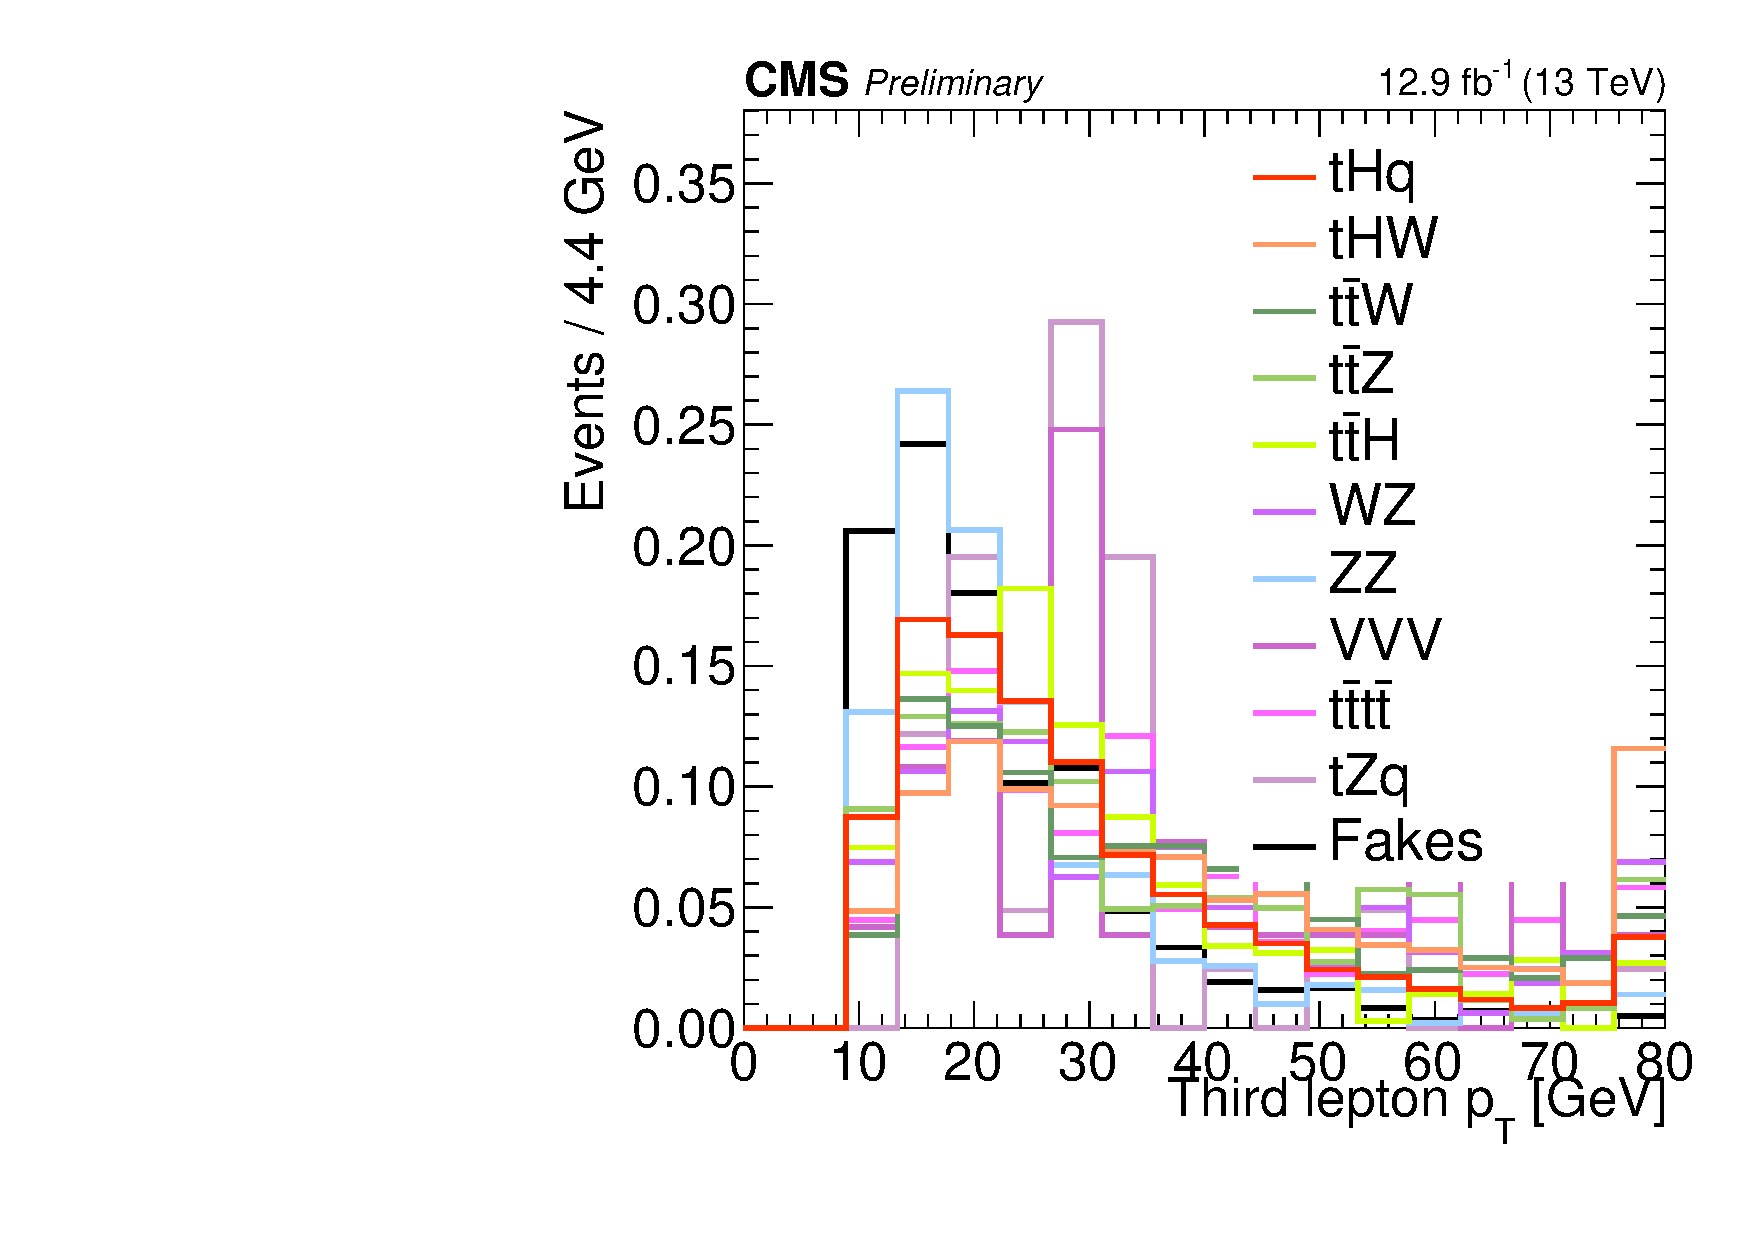
\includegraphics[width=0.245\textwidth]{figures/Lep3Pt.pdf} 
 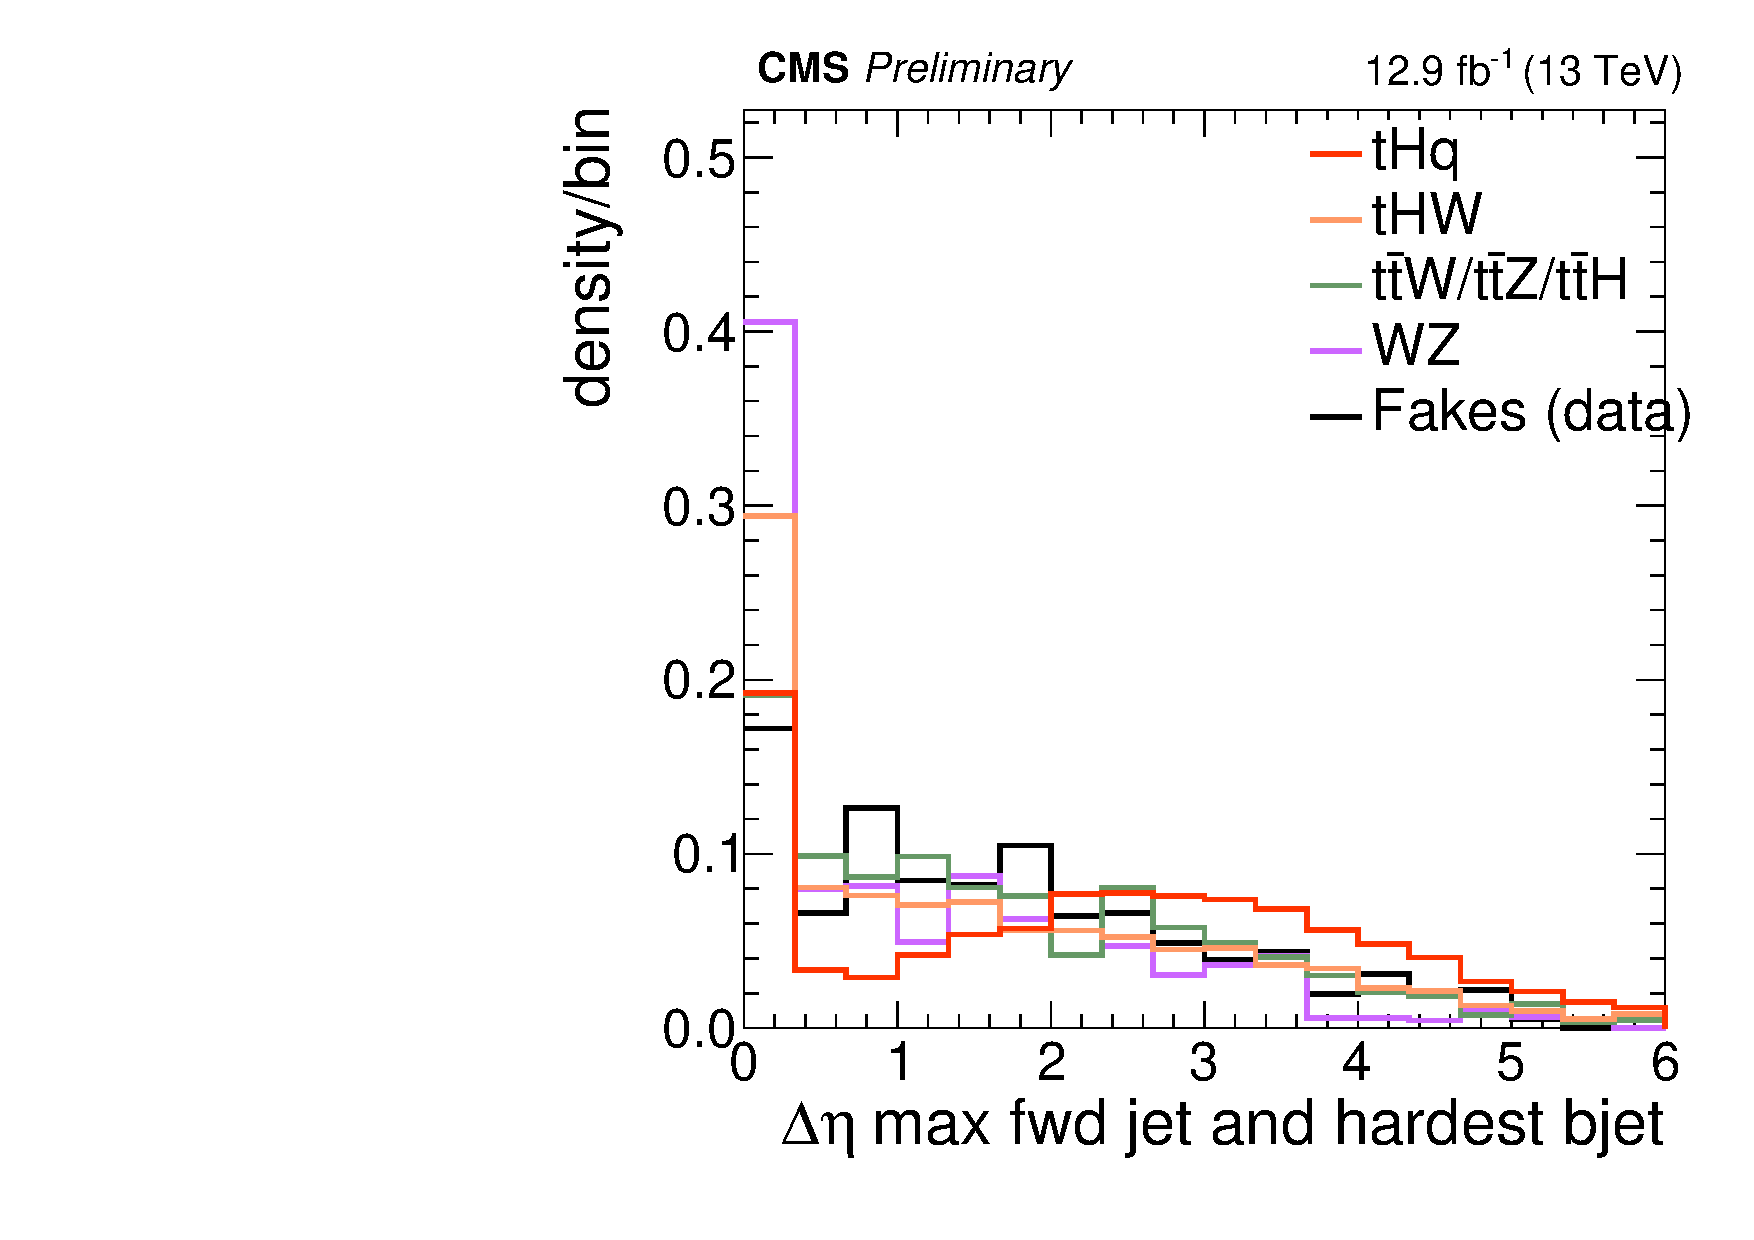
\includegraphics[width=0.245\textwidth]{figures/dEtaFwdJetBJet.pdf}
 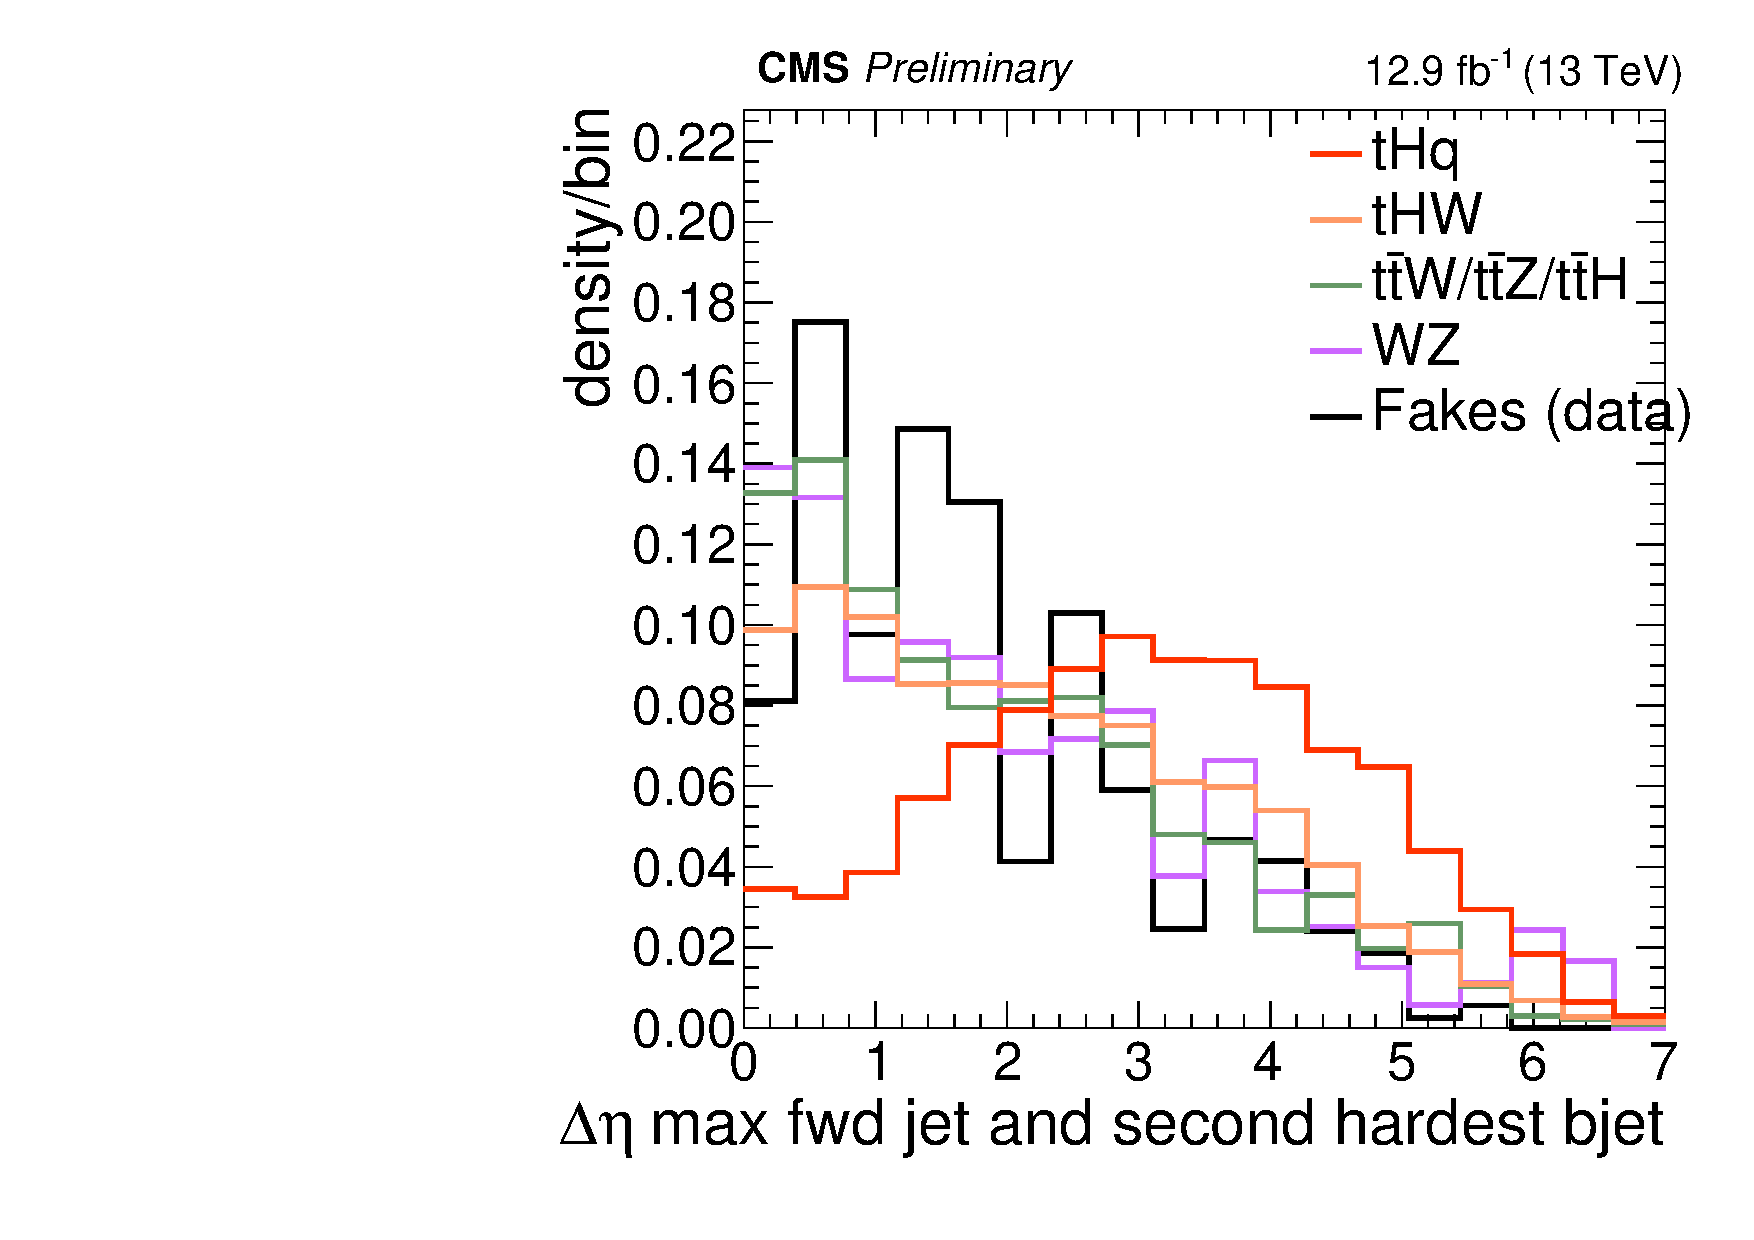
\includegraphics[width=0.245\textwidth]{figures/dEtaFwdJet2BJet.pdf}
 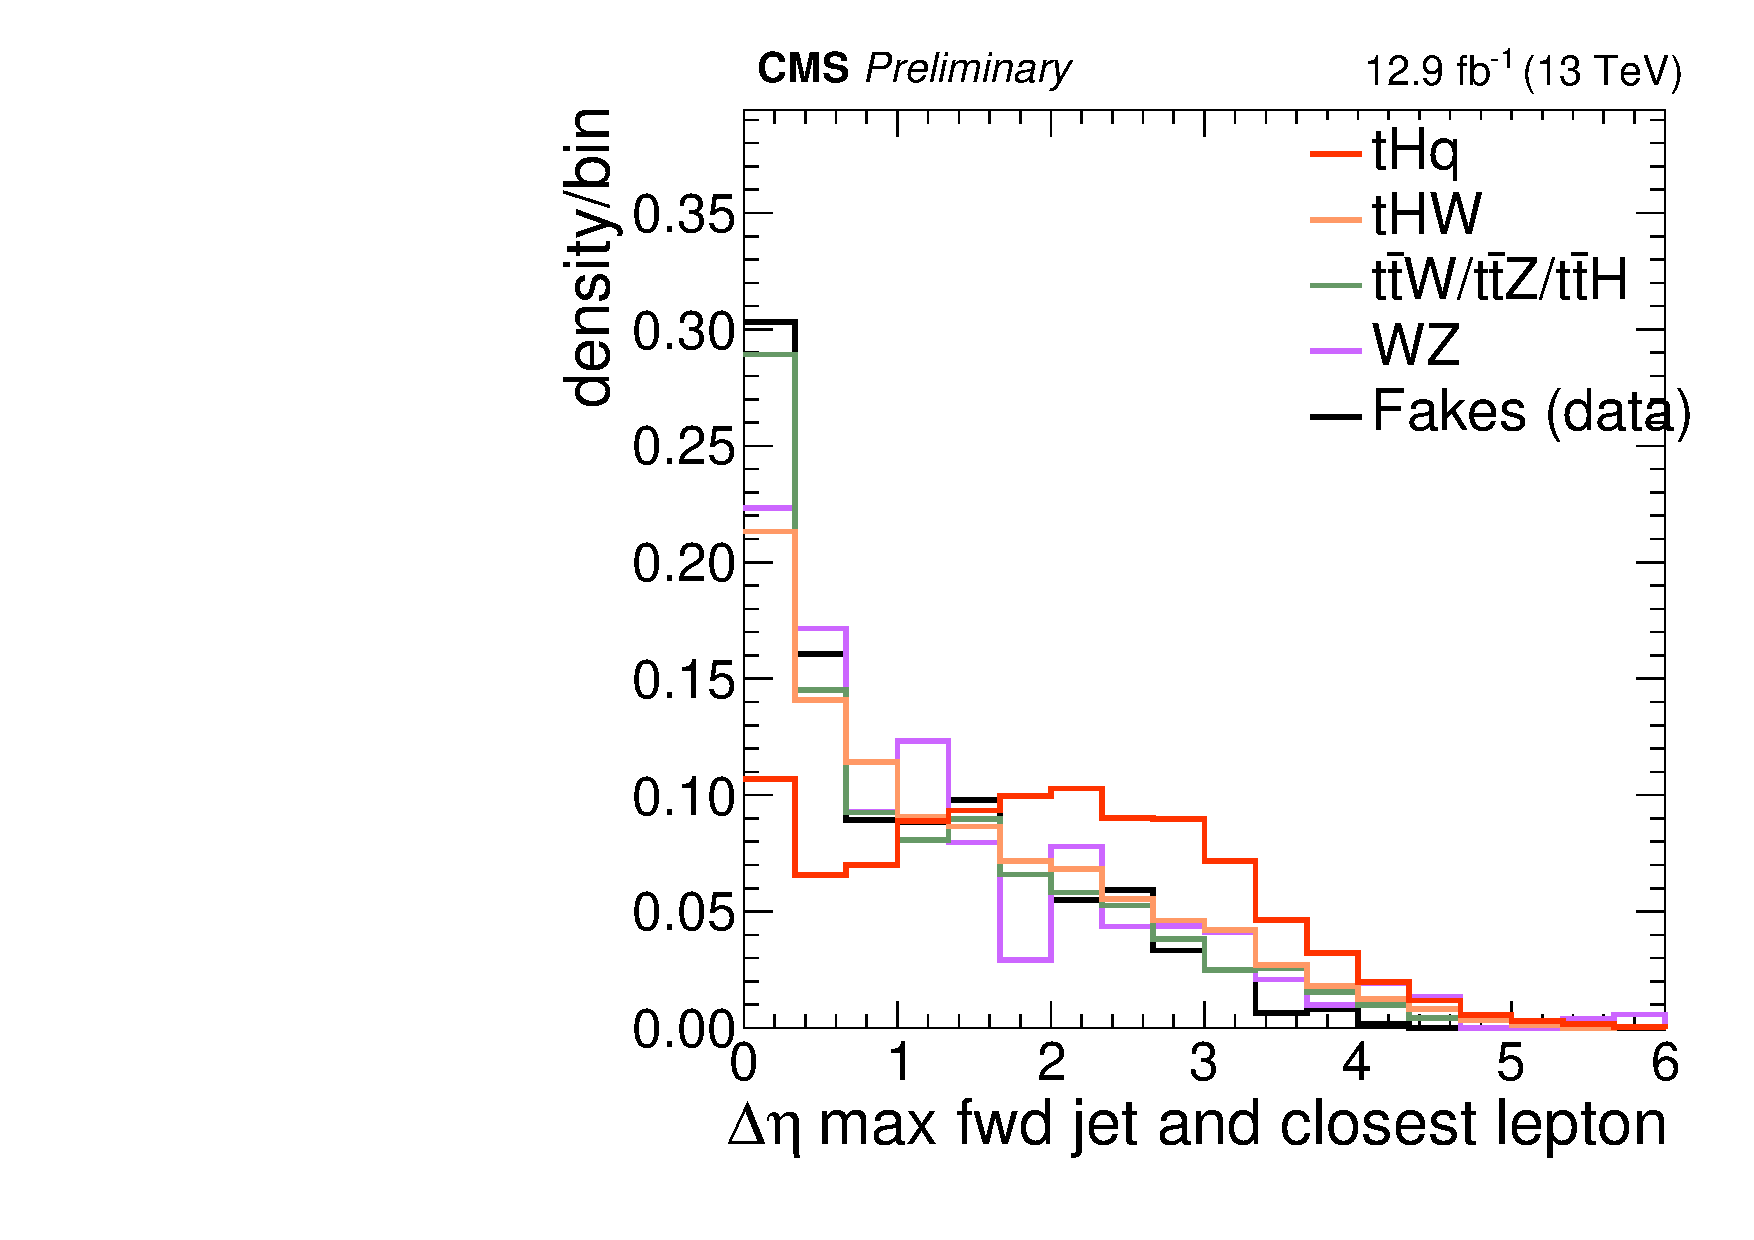
\includegraphics[width=0.245\textwidth]{figures/dEtaFwdJetClosestLep.pdf} \\
 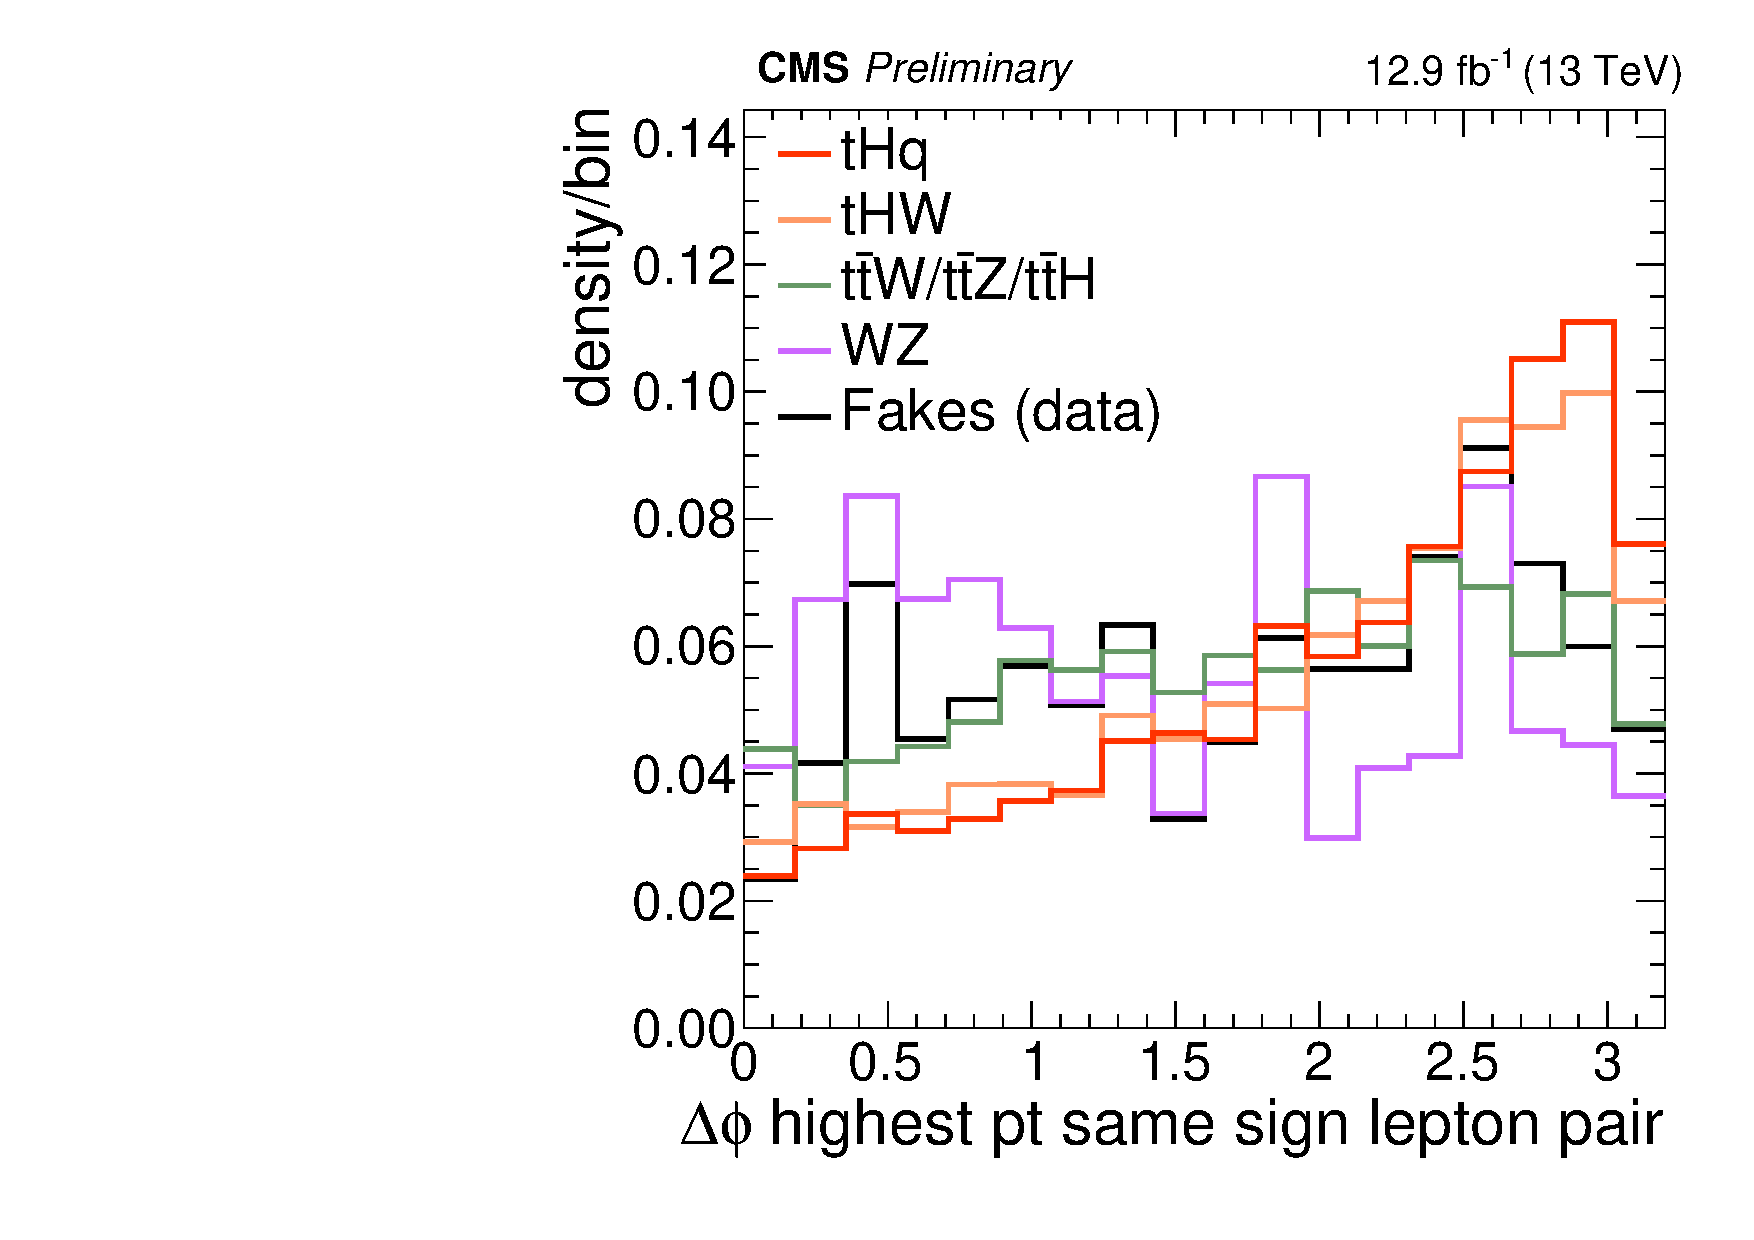
\includegraphics[width=0.245\textwidth]{figures/dPhiHighestPtSSPair.pdf}
 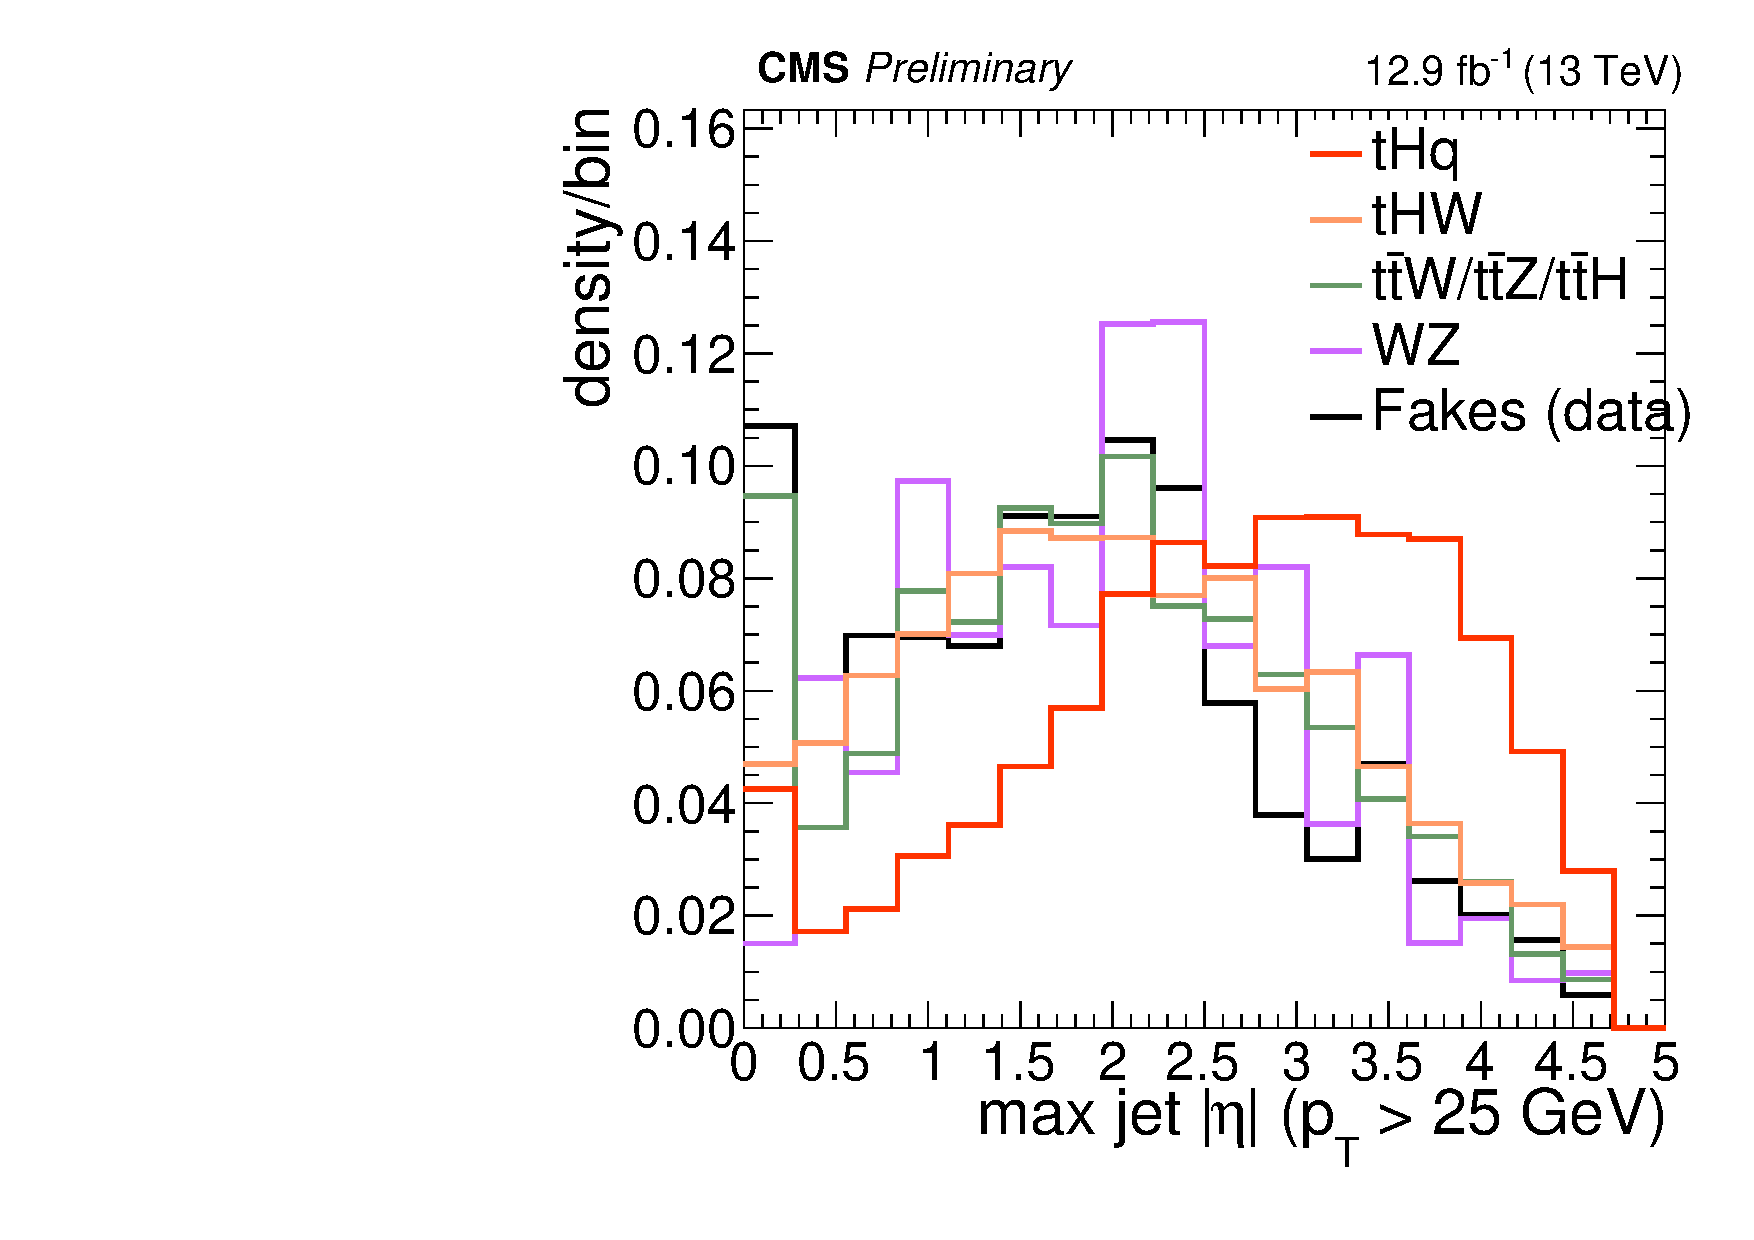
\includegraphics[width=0.245\textwidth]{figures/maxEtaJet25.pdf}
 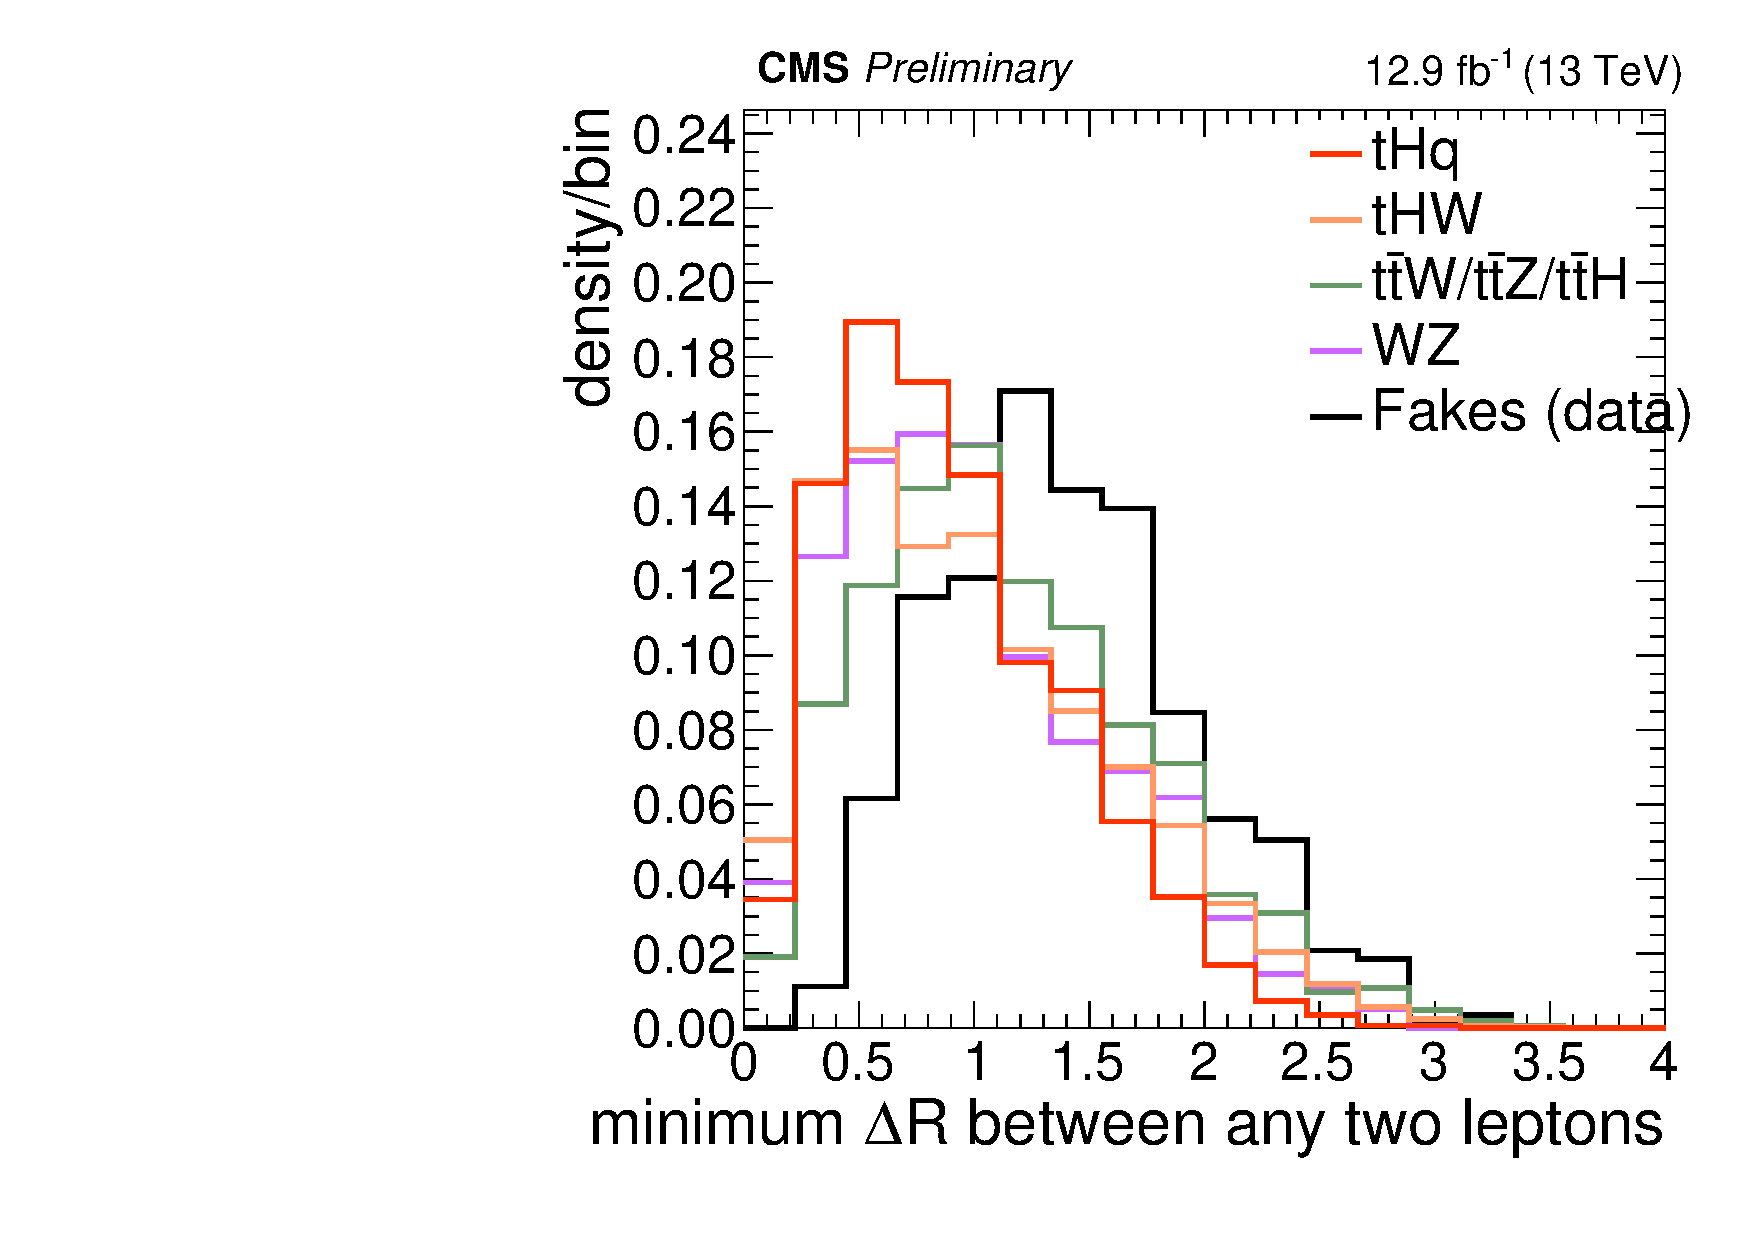
\includegraphics[width=0.245\textwidth]{figures/minDRll.pdf}
 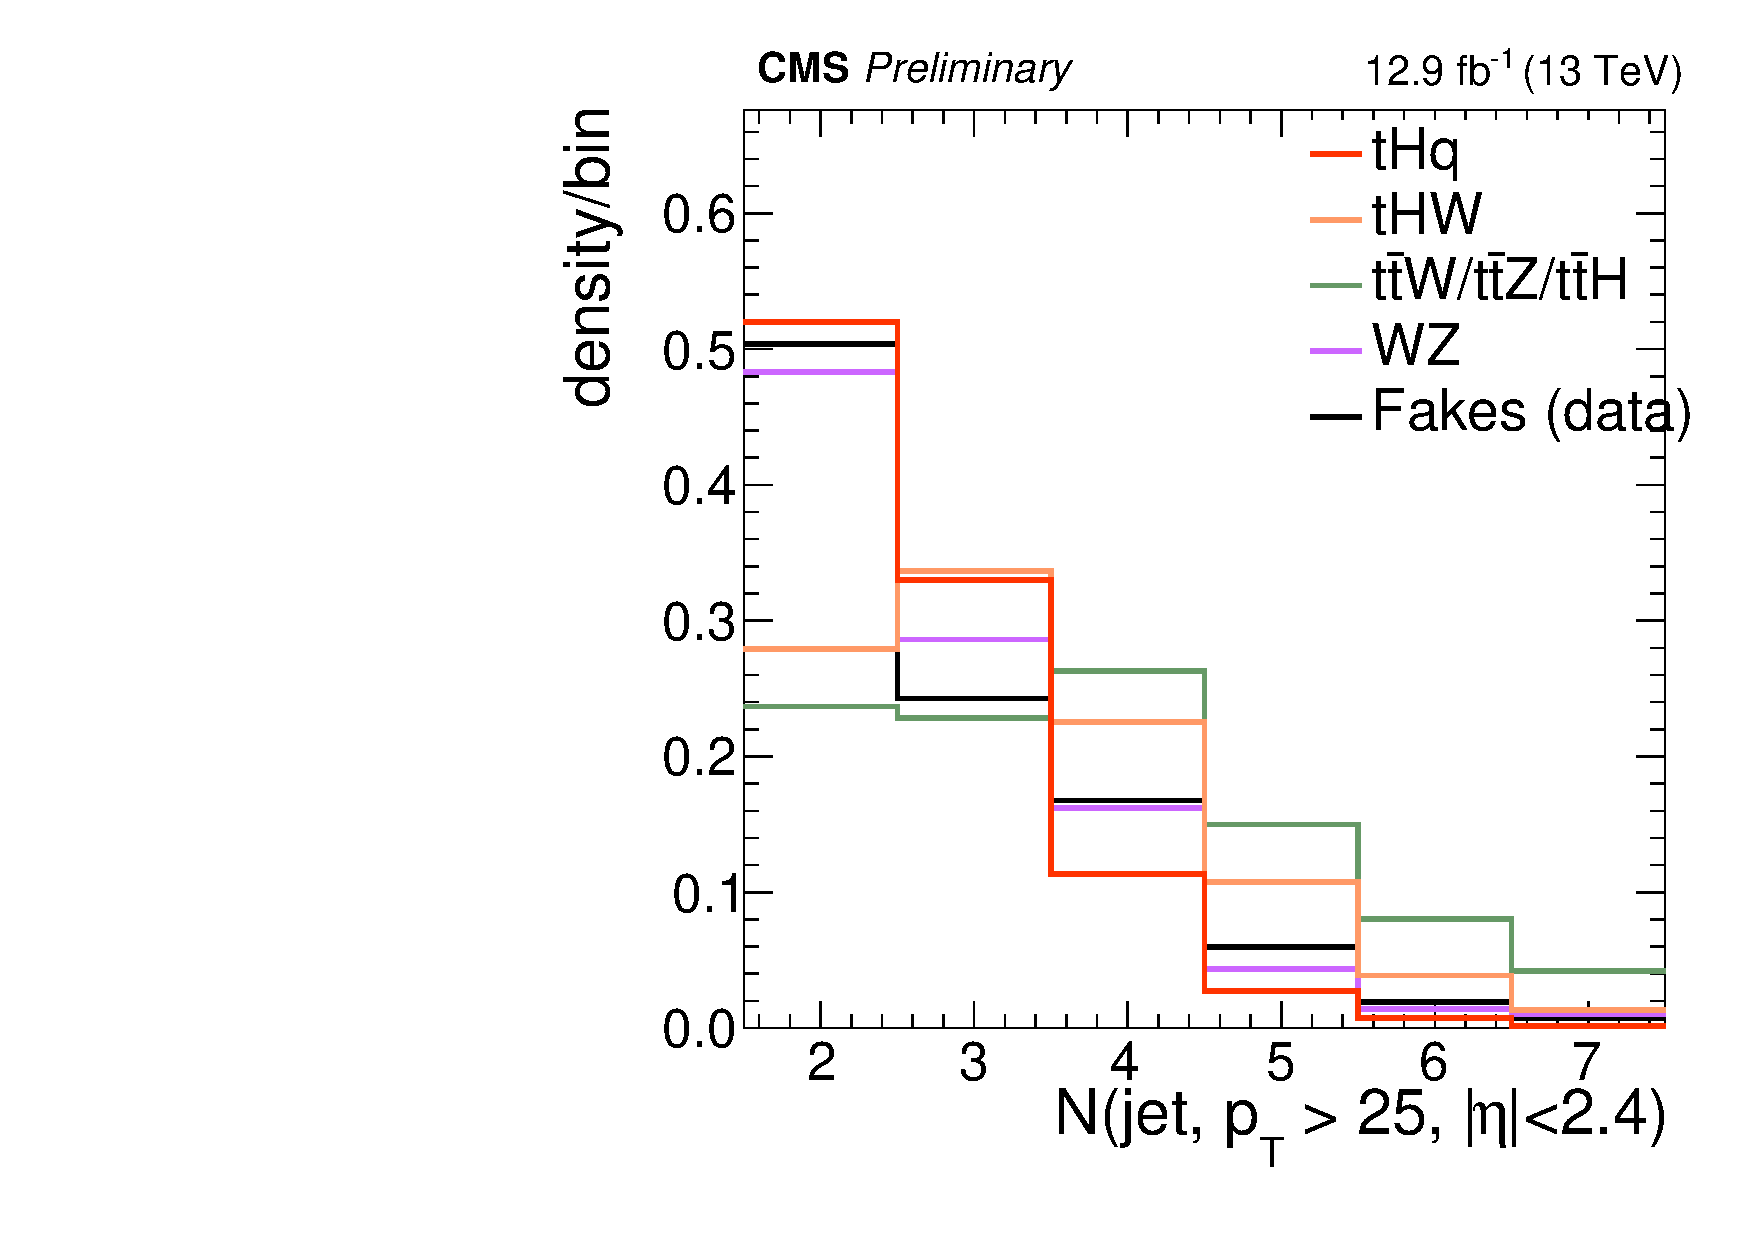
\includegraphics[width=0.245\textwidth]{figures/nJet25.pdf} \\
 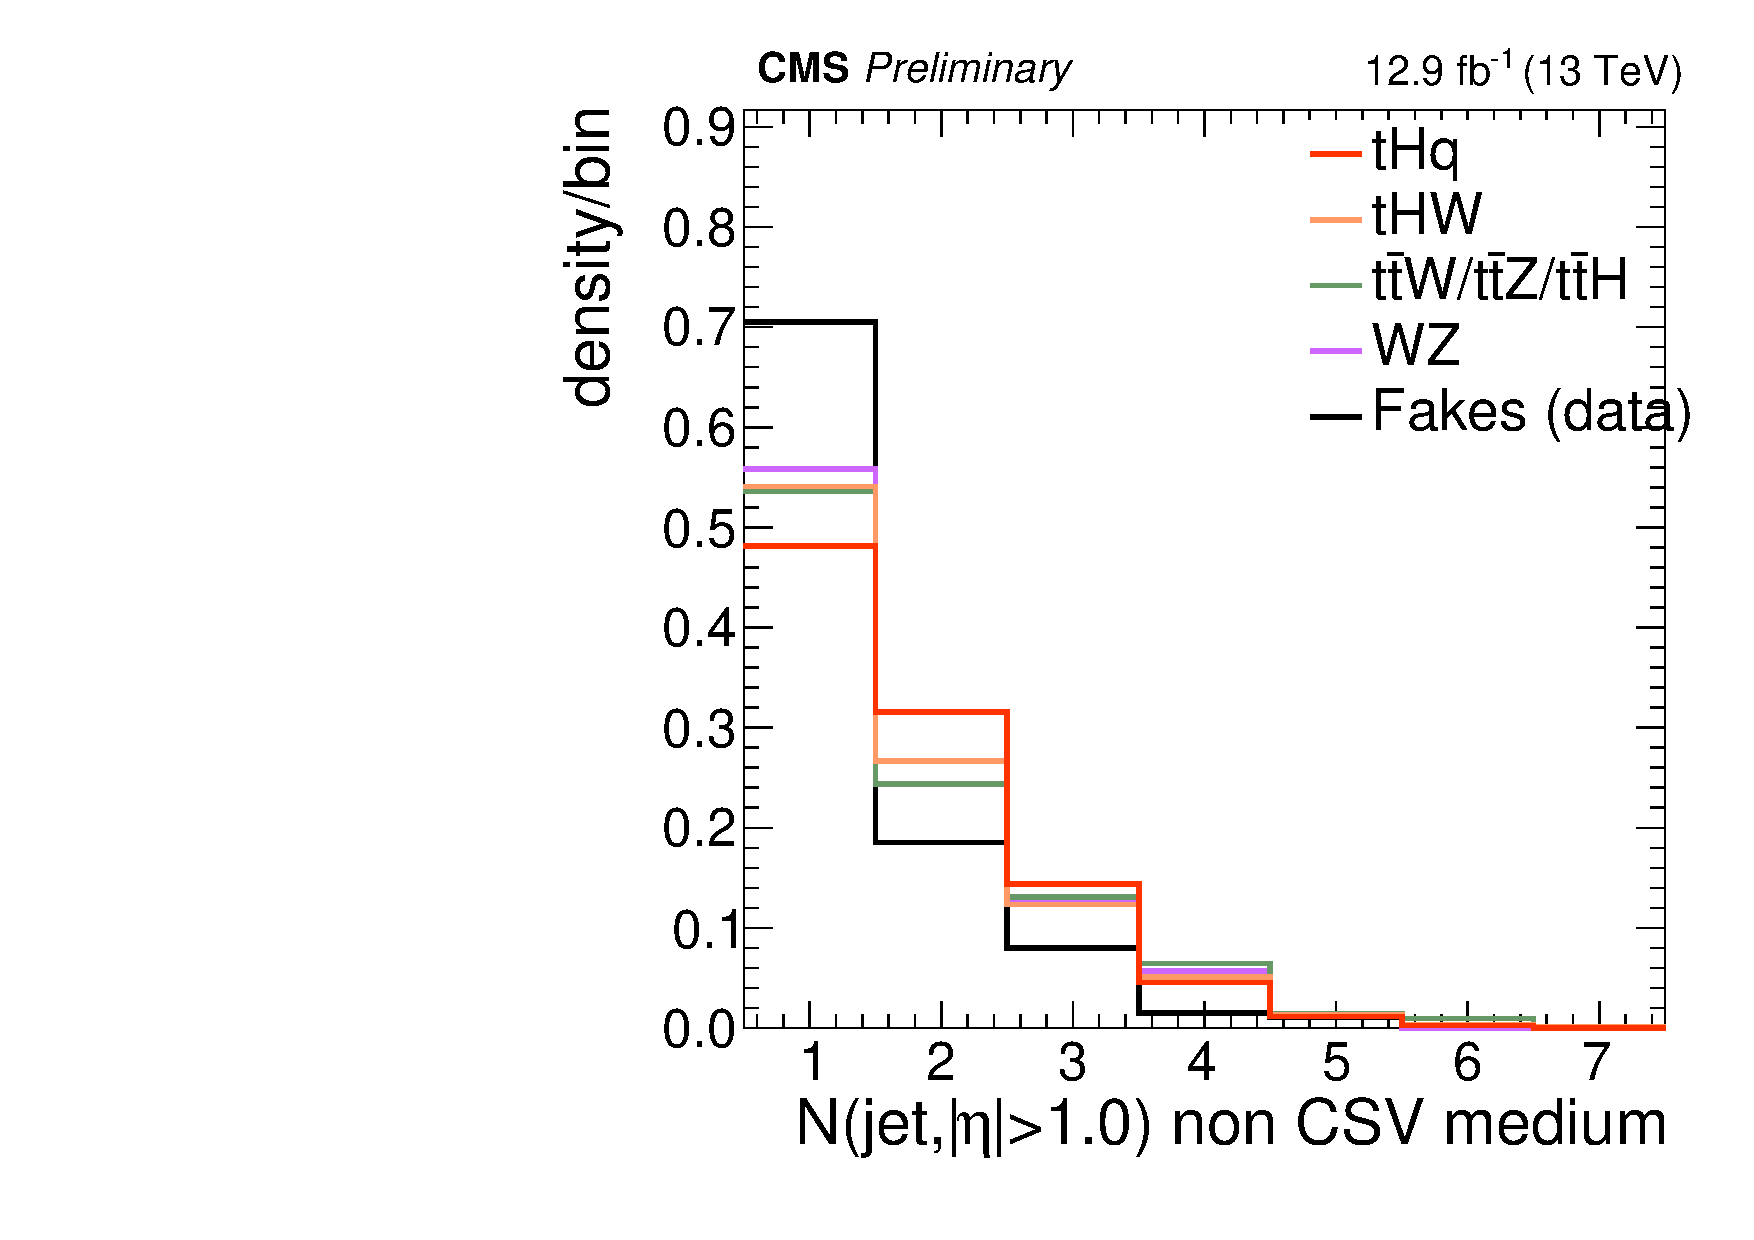
\includegraphics[width=0.245\textwidth]{figures/nJetEta1.pdf}
 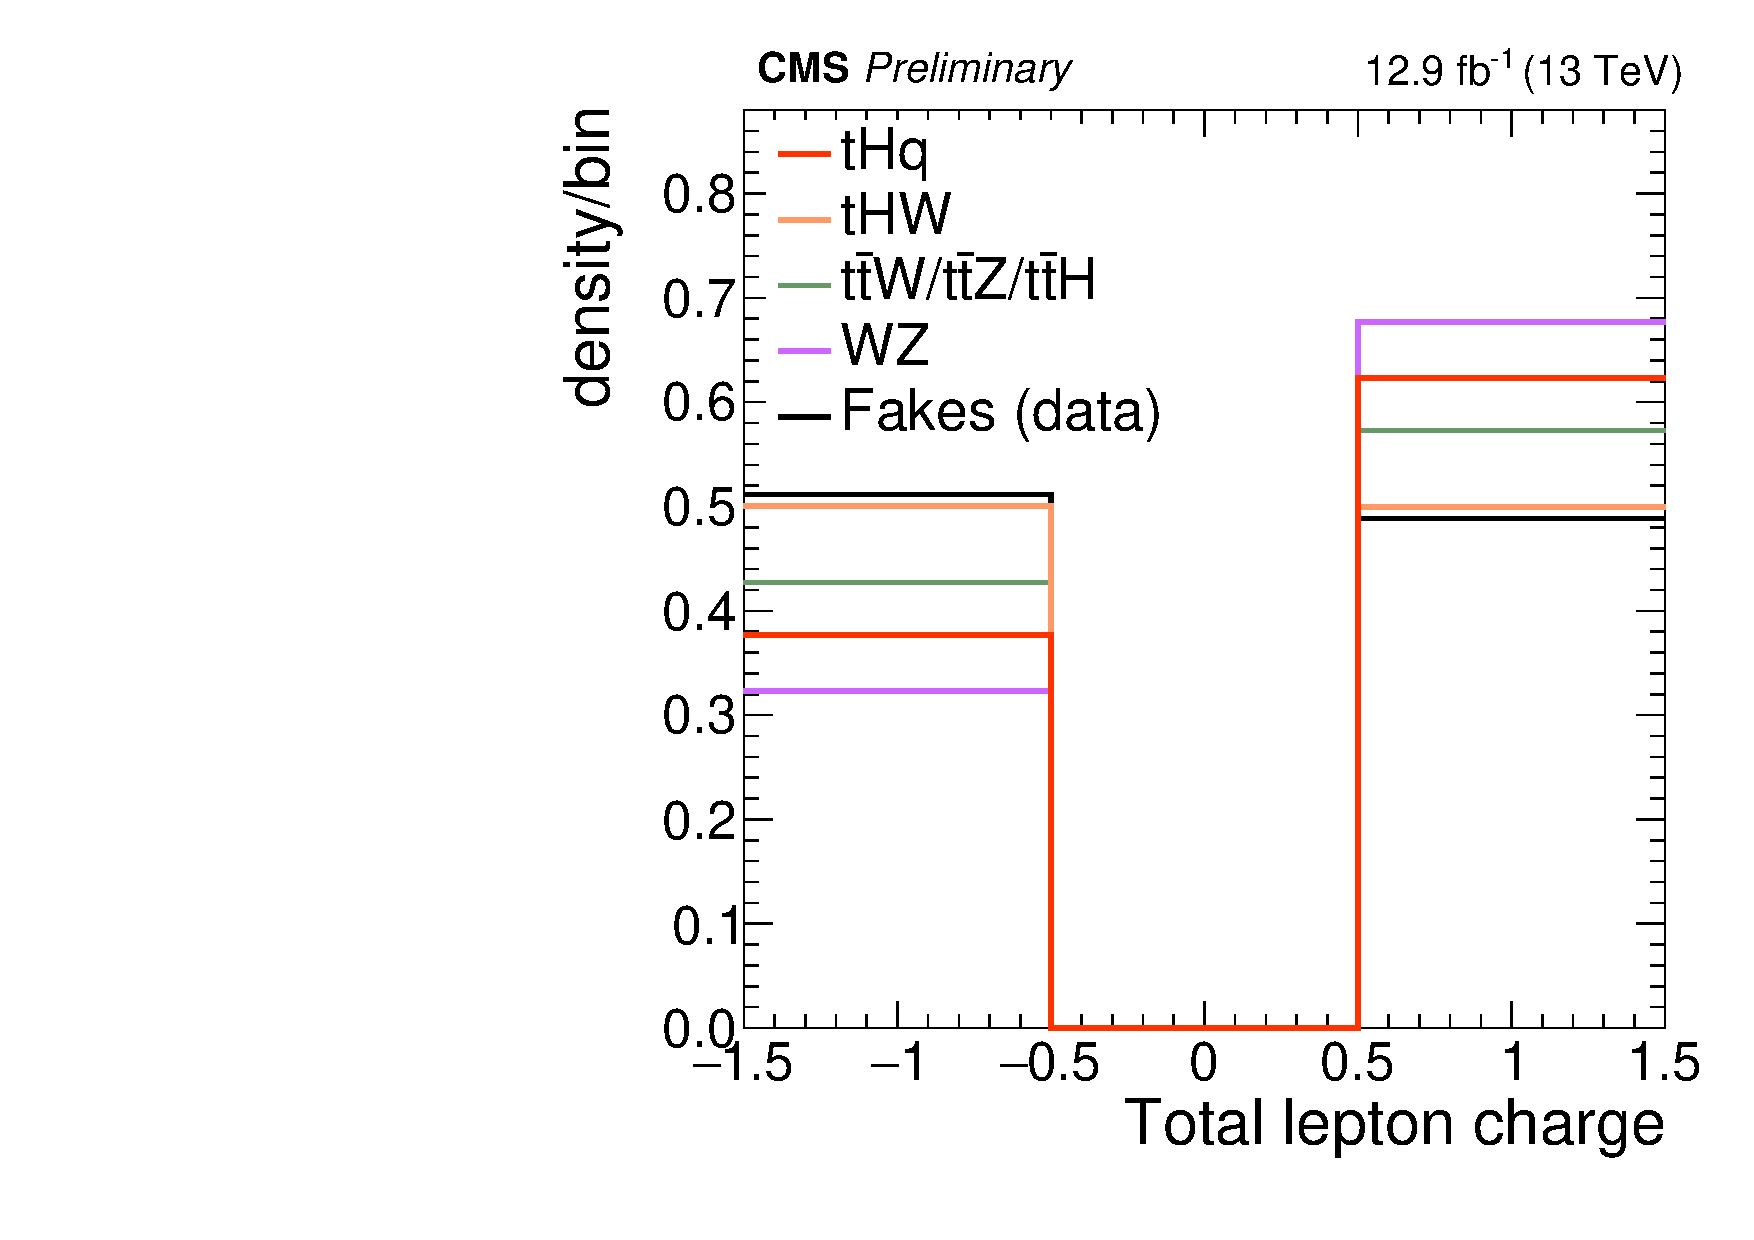
\includegraphics[width=0.245\textwidth]{figures/totCharge.pdf}
\caption{Distributions of input variables to the BDT for signal discrimination, three lepton channel.} 
\label{fig:input_vars_3l}
\end{figure}    

\begin{figure} [!h]
  \centering
  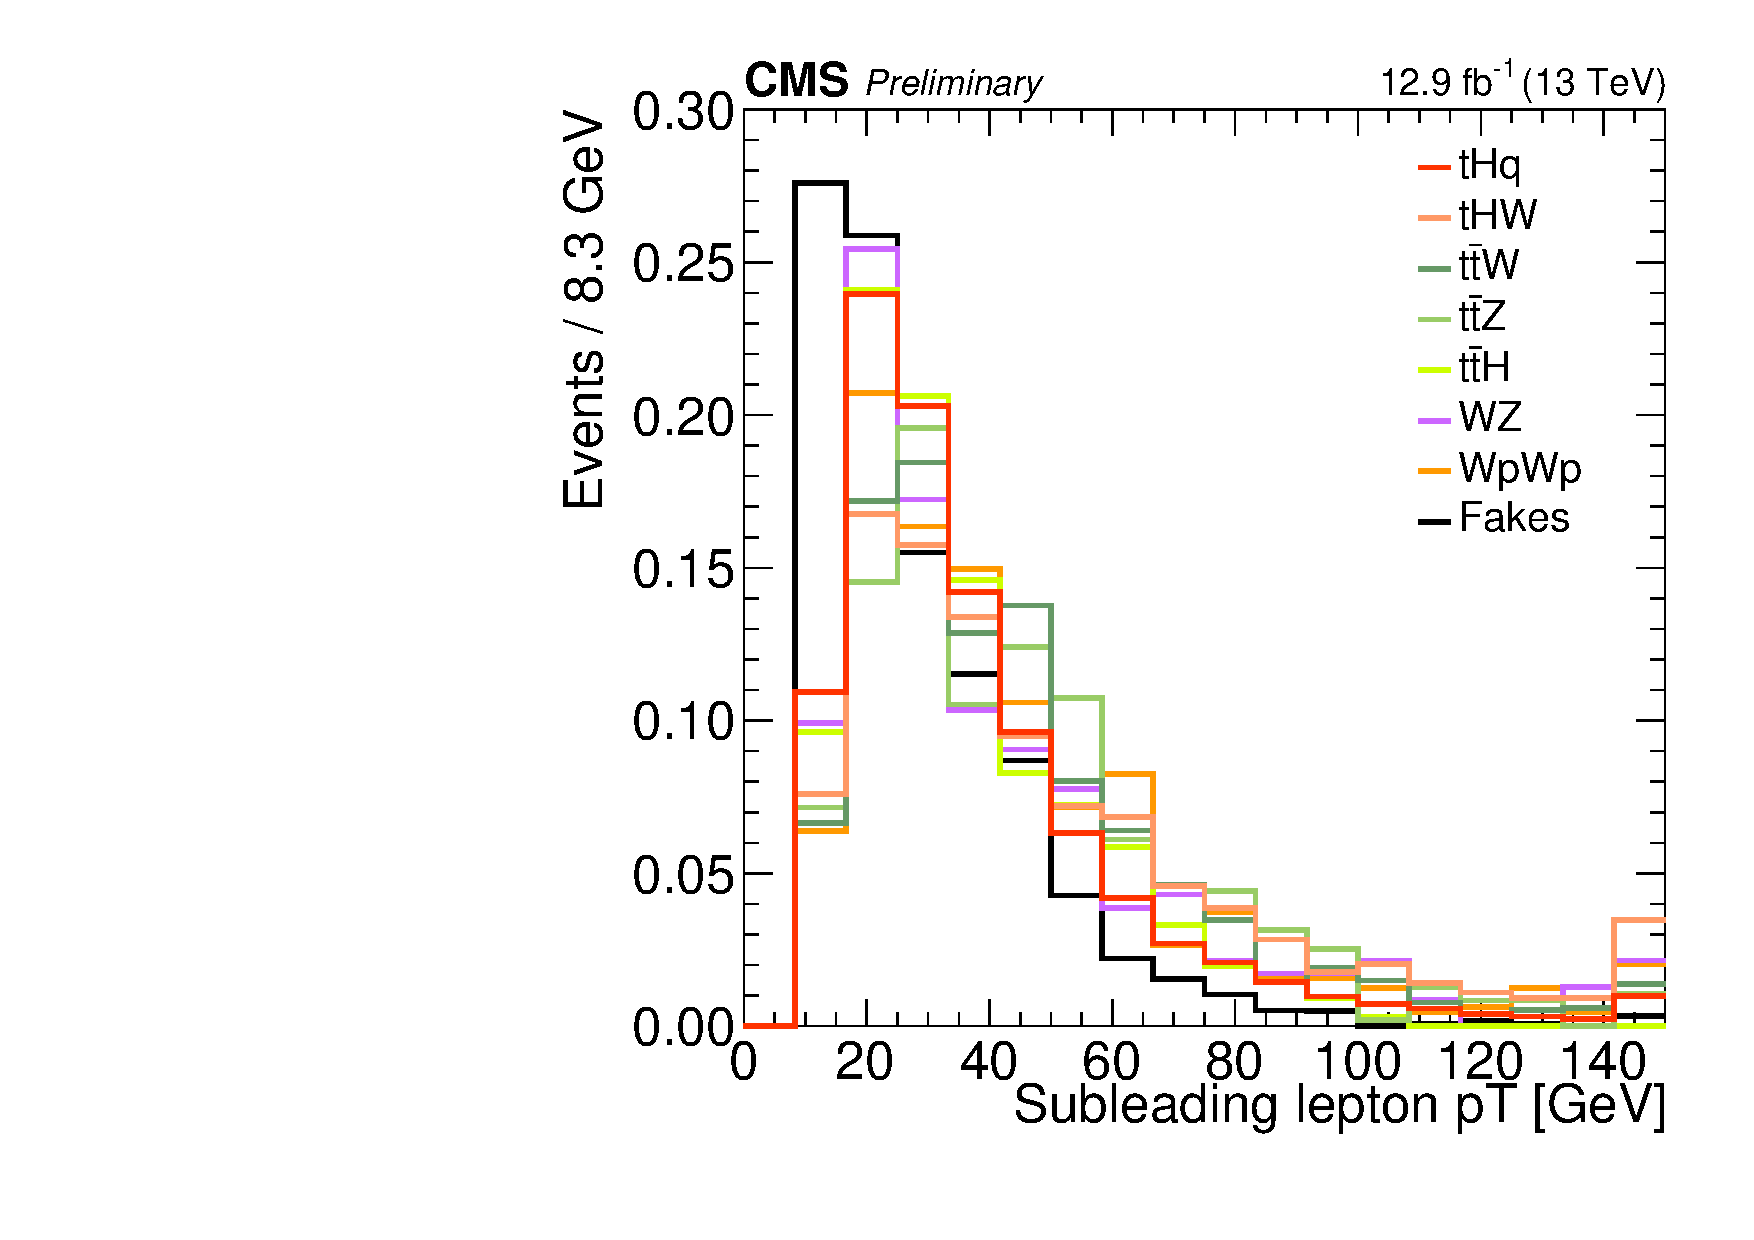
\includegraphics[width=0.245\textwidth]{figures/Lep2Pt_mumu.pdf} 
  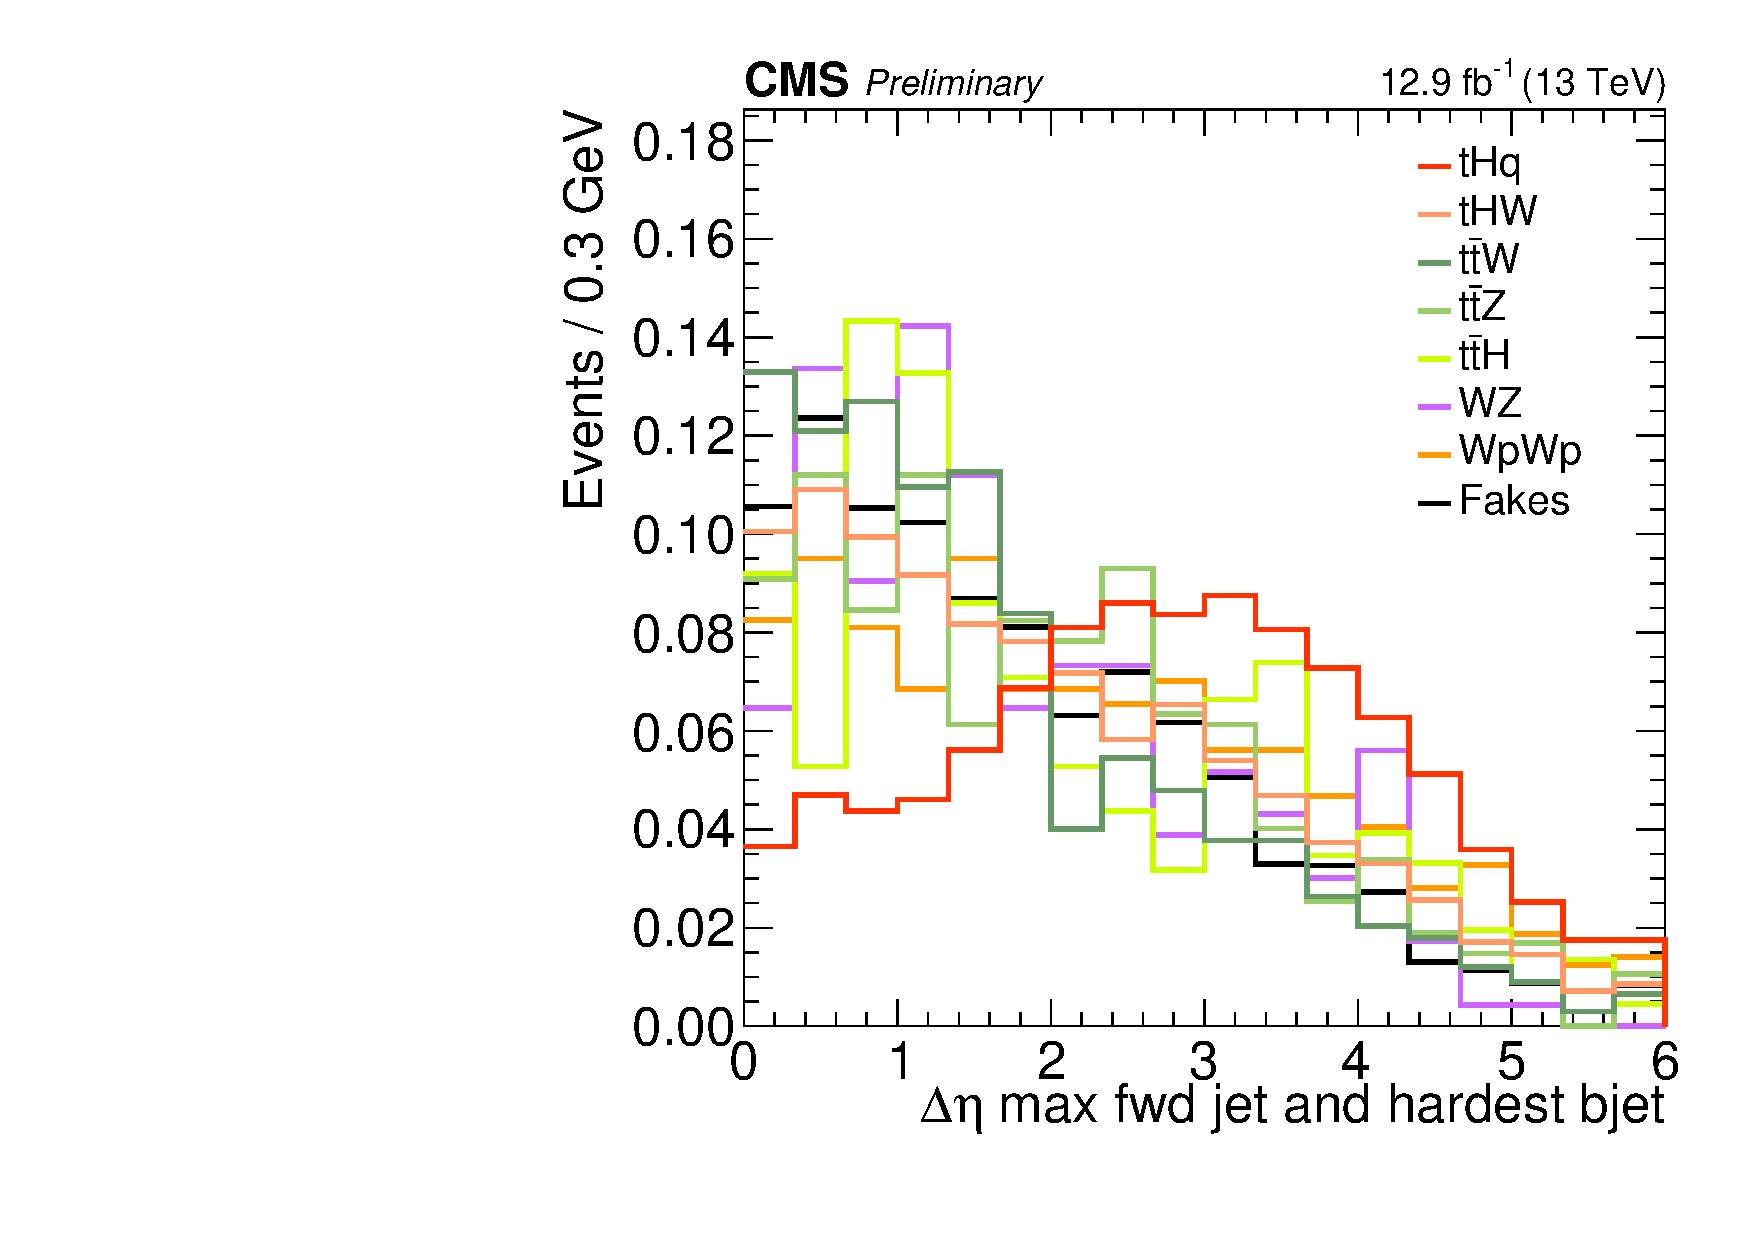
\includegraphics[width=0.245\textwidth]{figures/dEtaFwdJetBJet_mumu.pdf}
  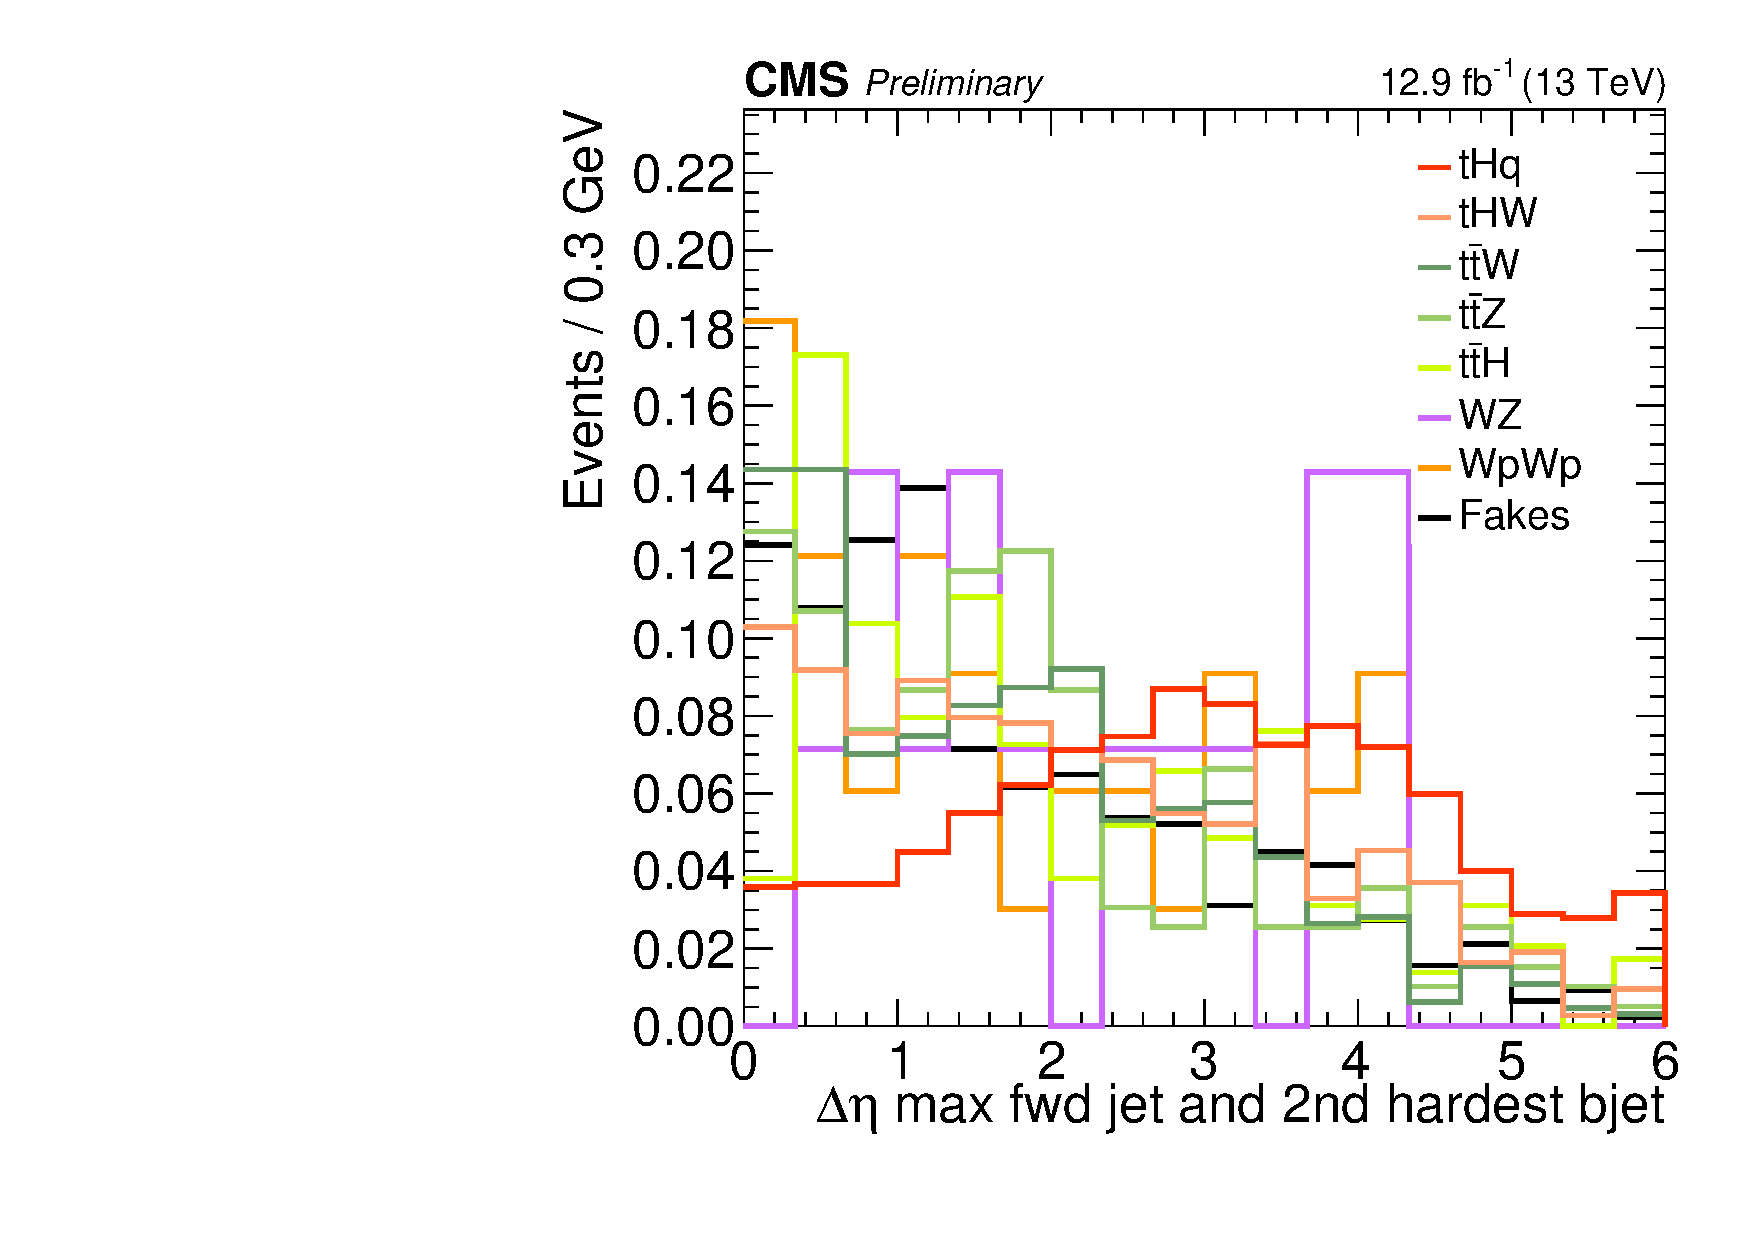
\includegraphics[width=0.245\textwidth]{figures/dEtaFwdJet2BJet_mumu.pdf}
  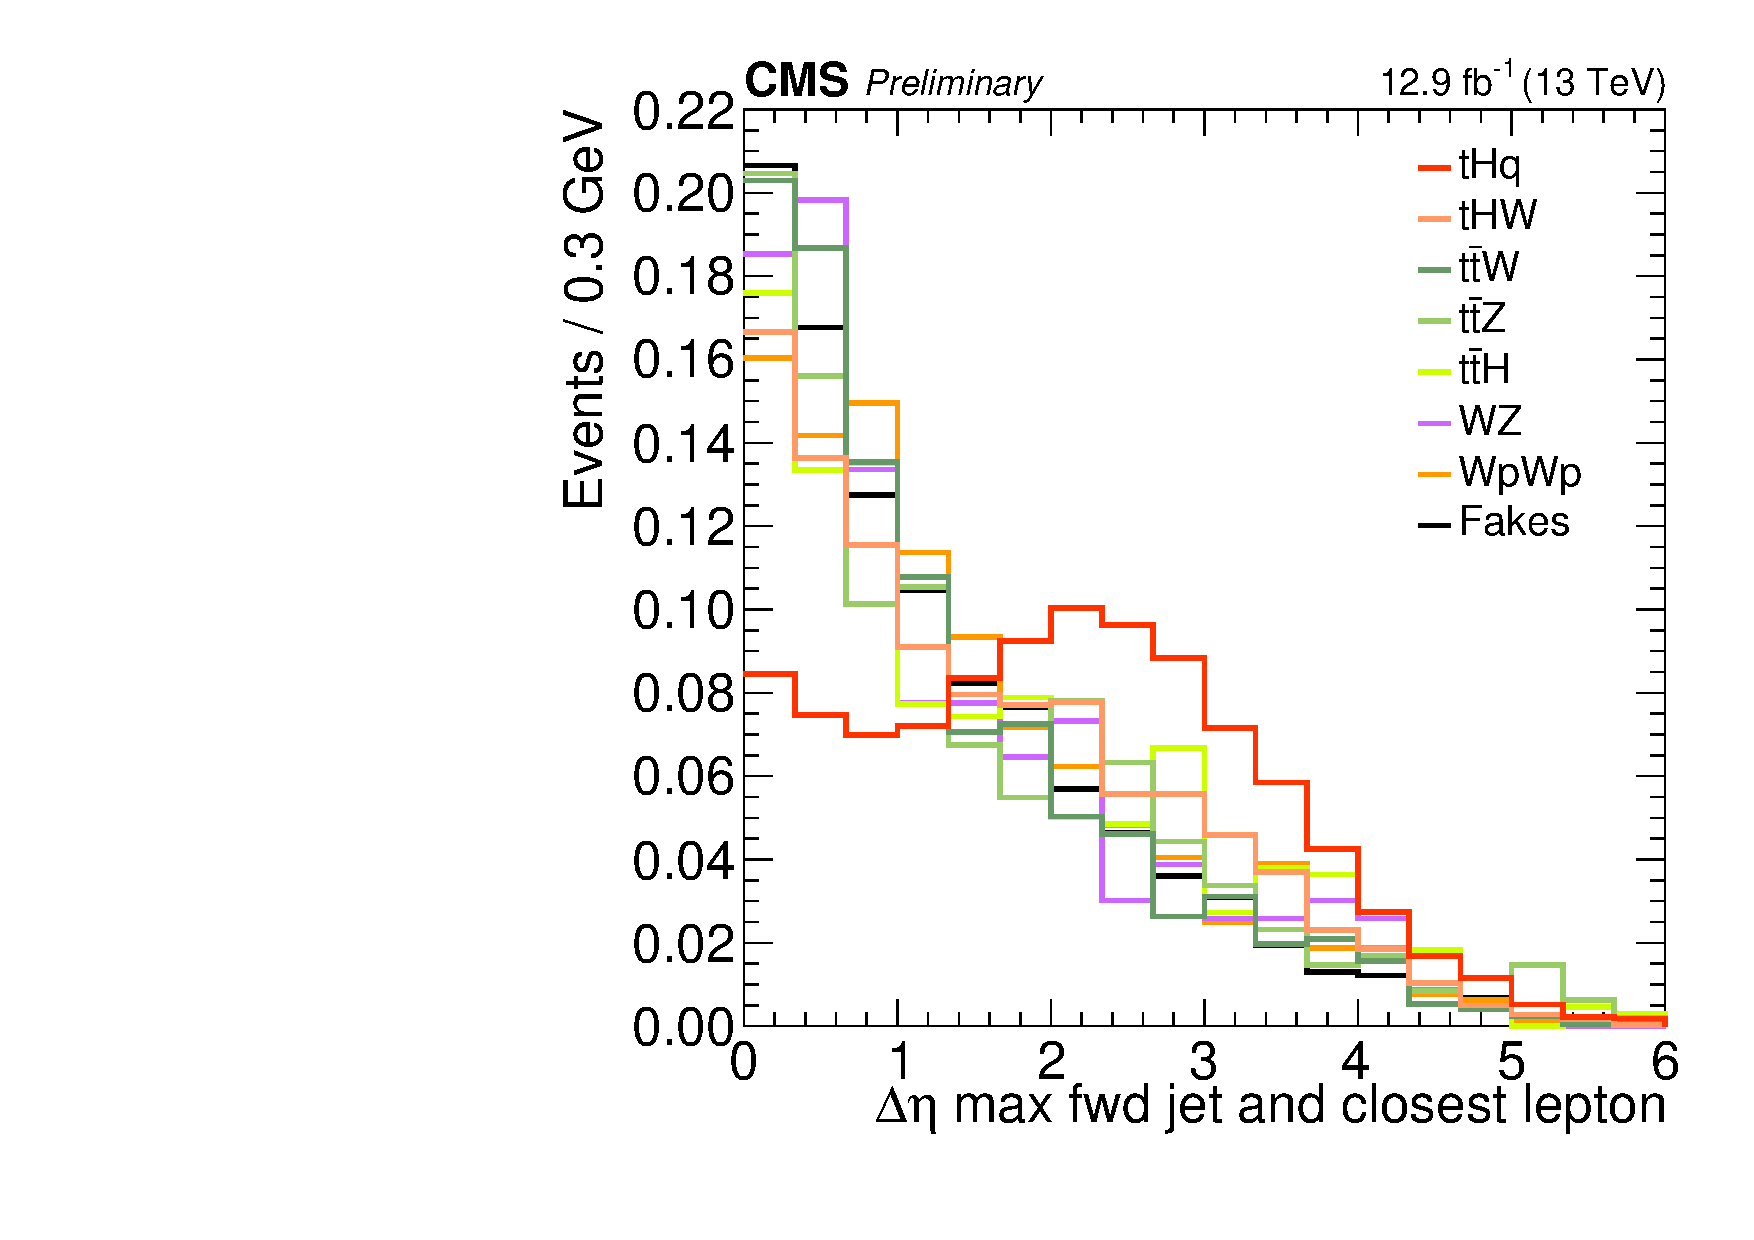
\includegraphics[width=0.245\textwidth]{figures/dEtaFwdJetClosestLep_mumu.pdf} \\
  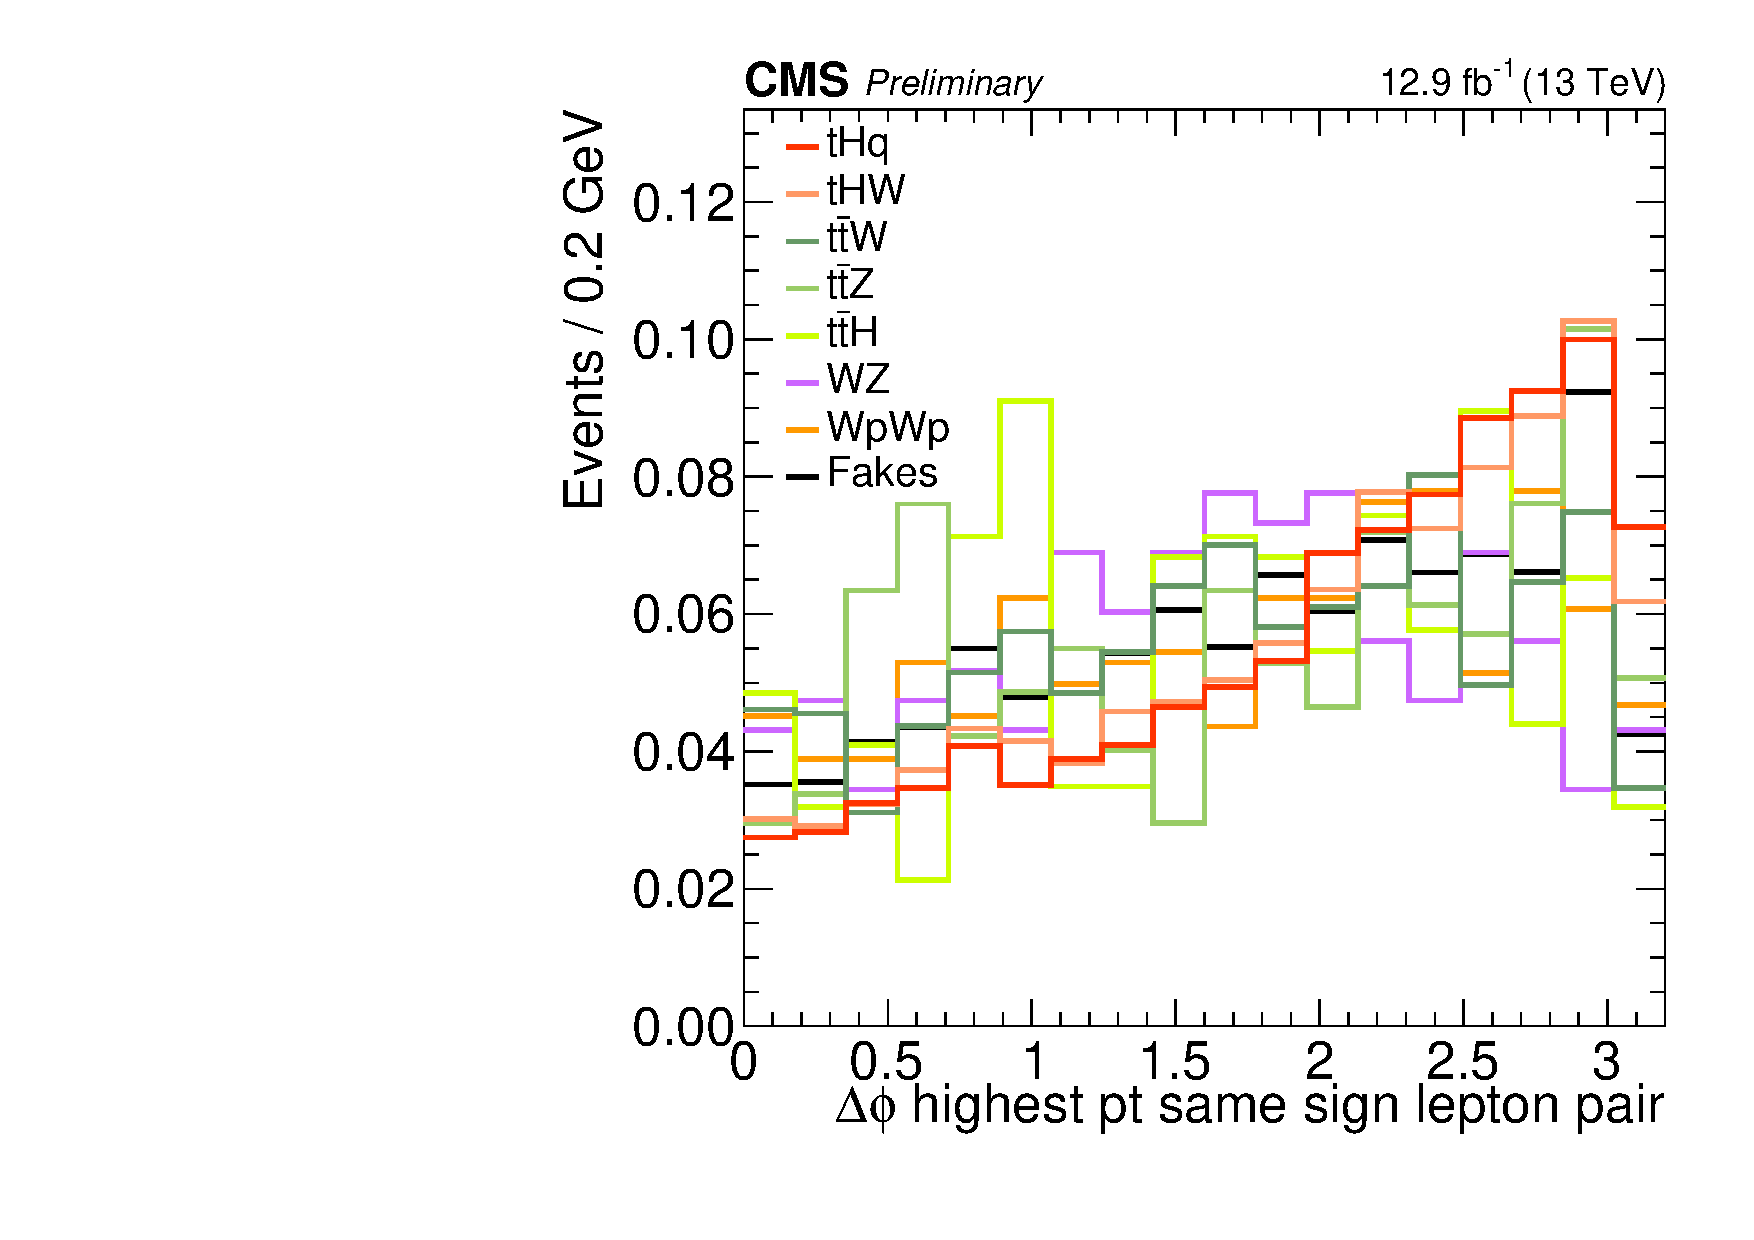
\includegraphics[width=0.245\textwidth]{figures/dPhiHighestPtSSPair_mumu.pdf}
  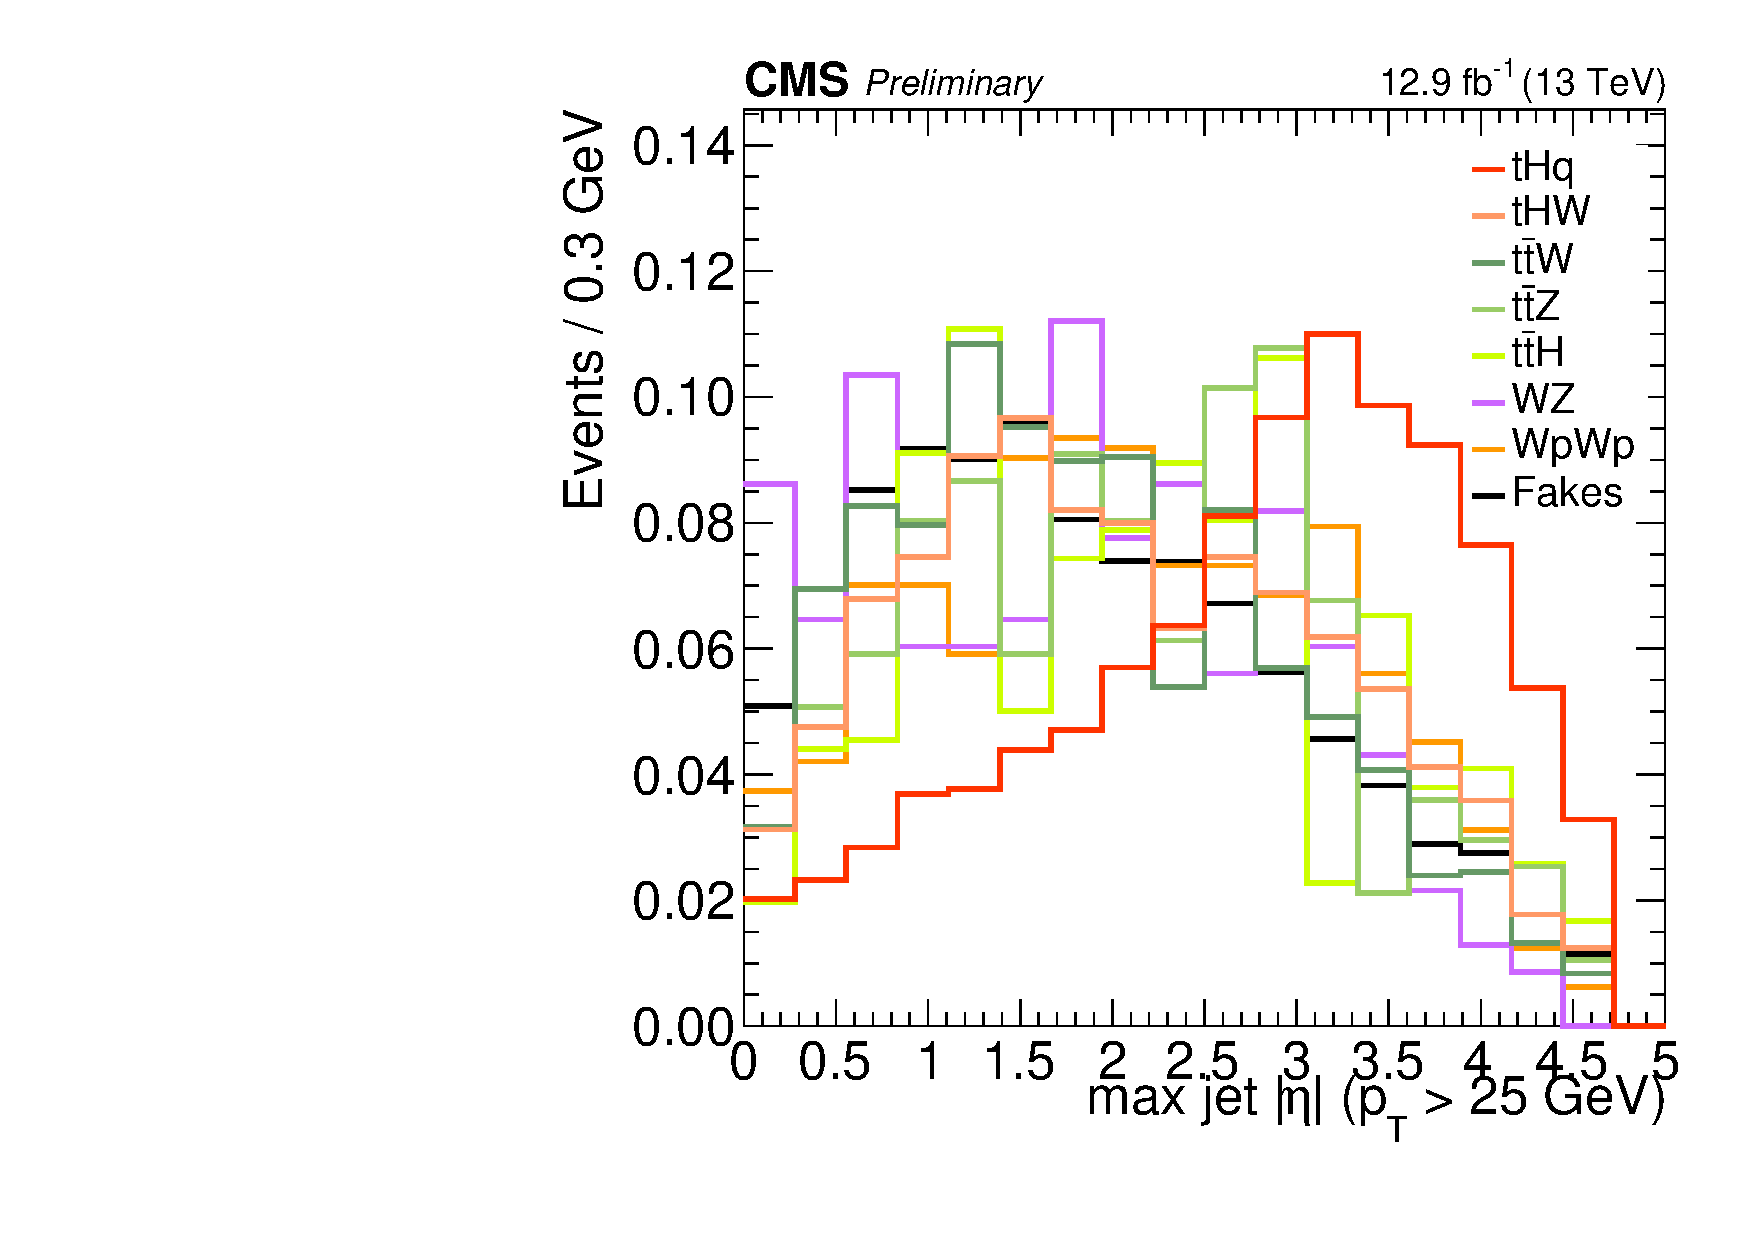
\includegraphics[width=0.245\textwidth]{figures/maxEtaJet25_mumu.pdf}
  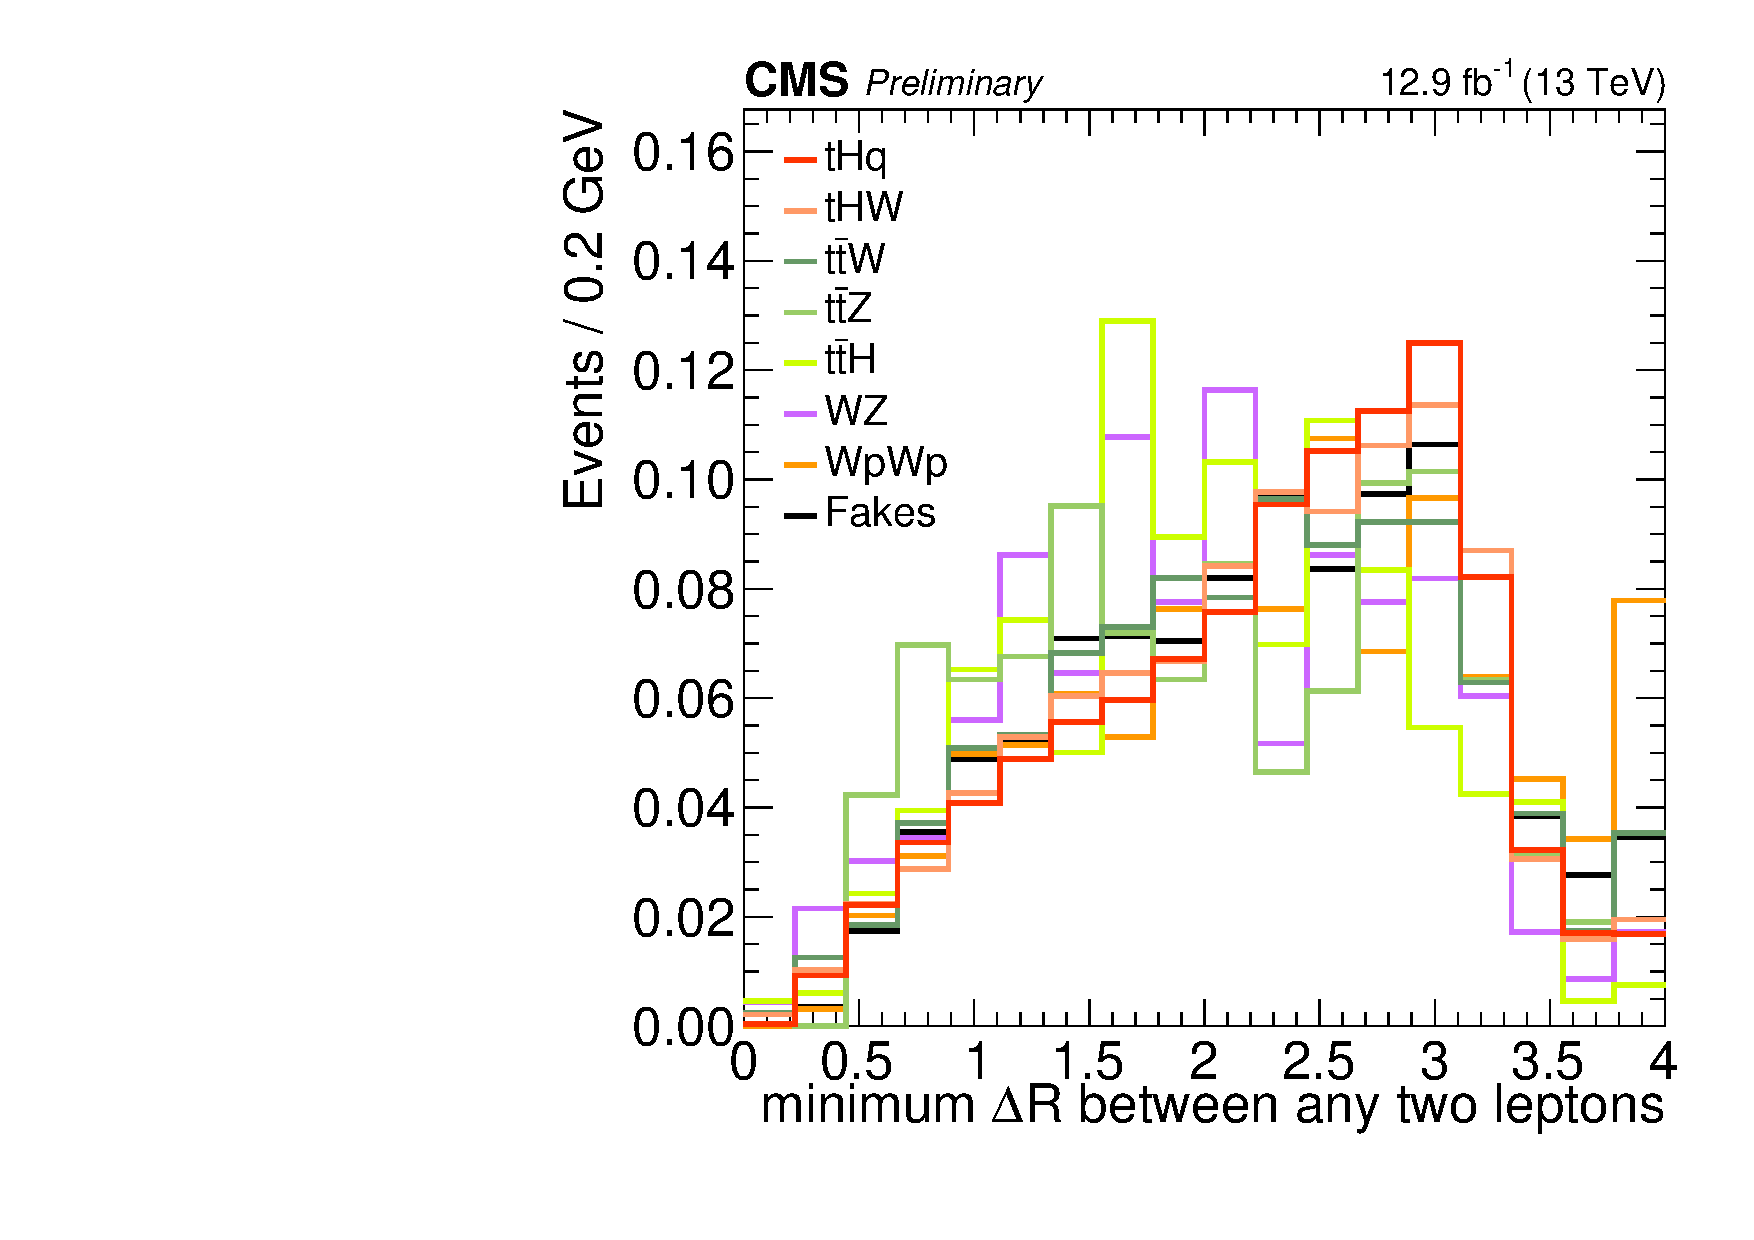
\includegraphics[width=0.245\textwidth]{figures/minDRll_mumu.pdf}
  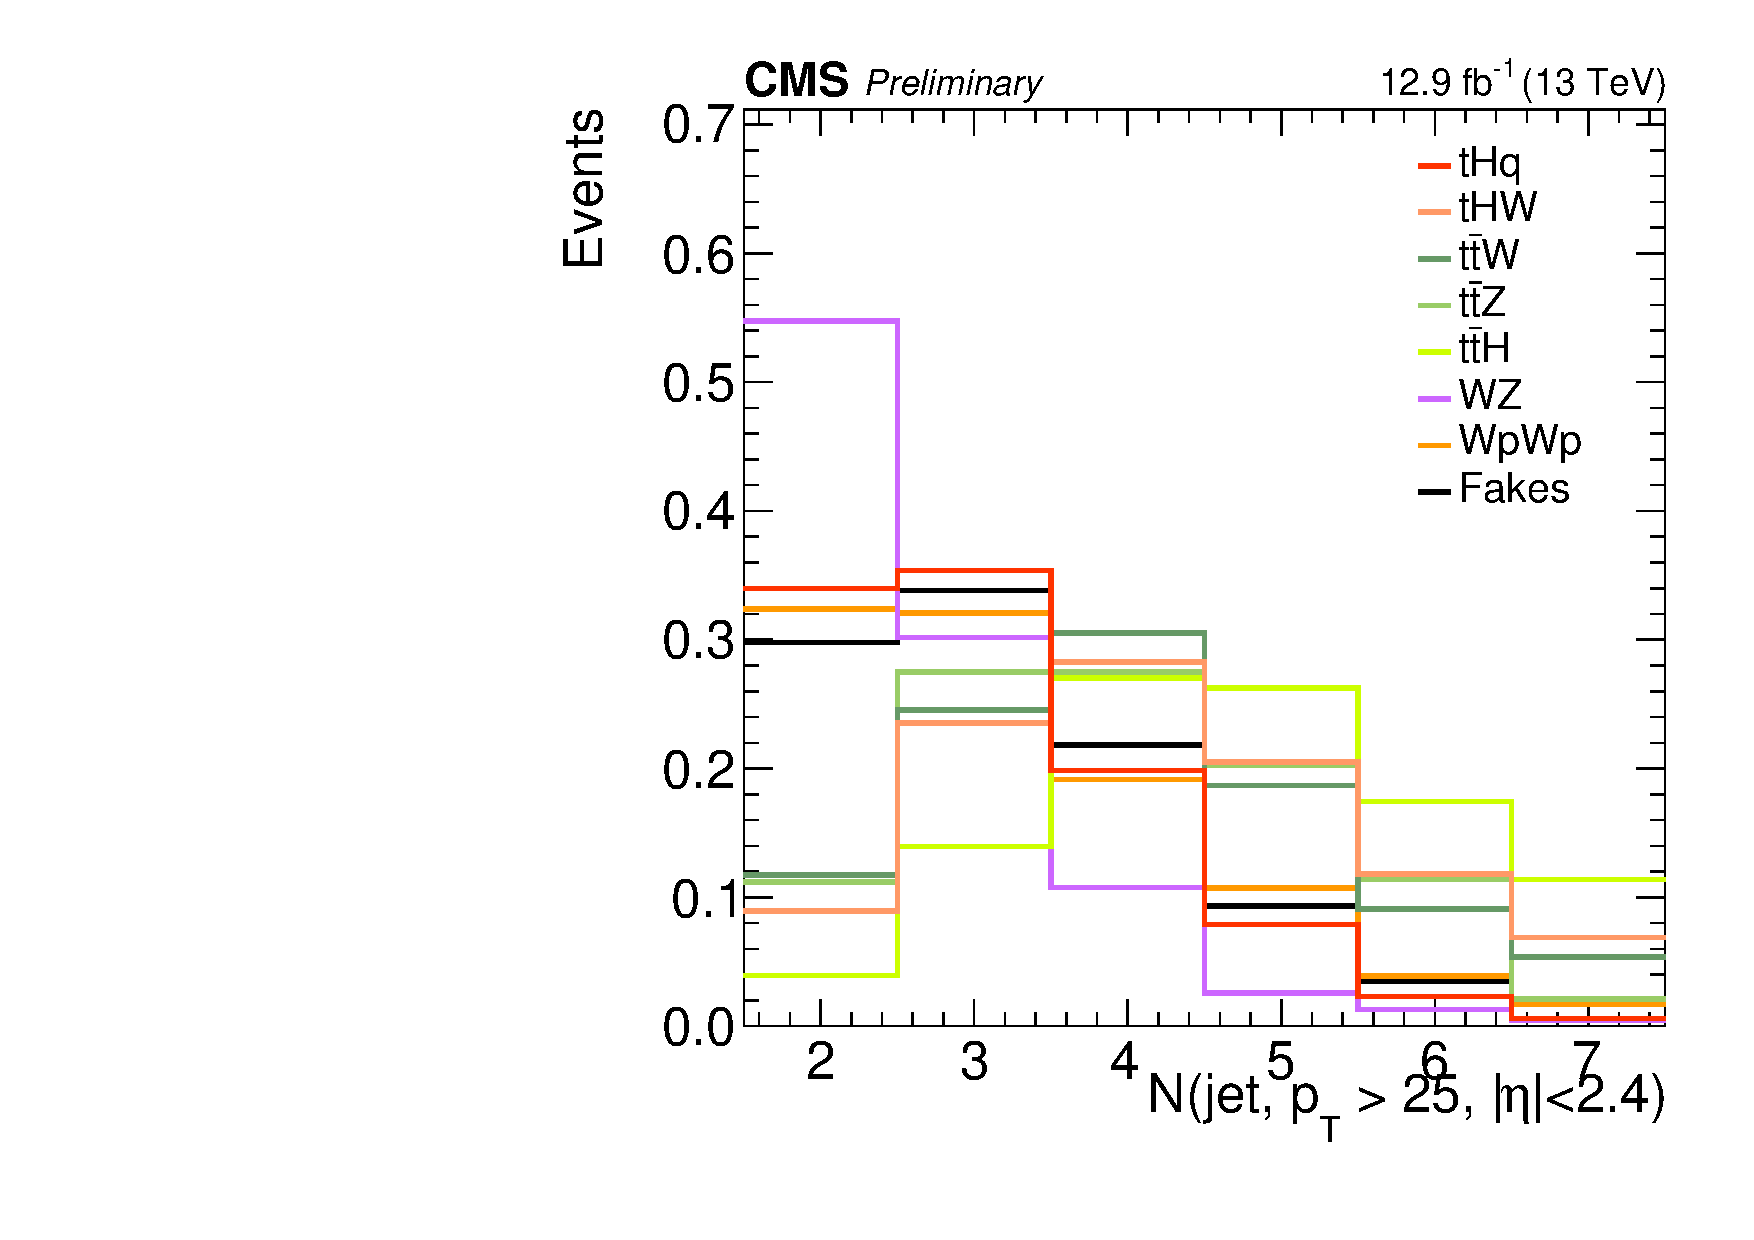
\includegraphics[width=0.245\textwidth]{figures/nJet25_mumu.pdf} \\
  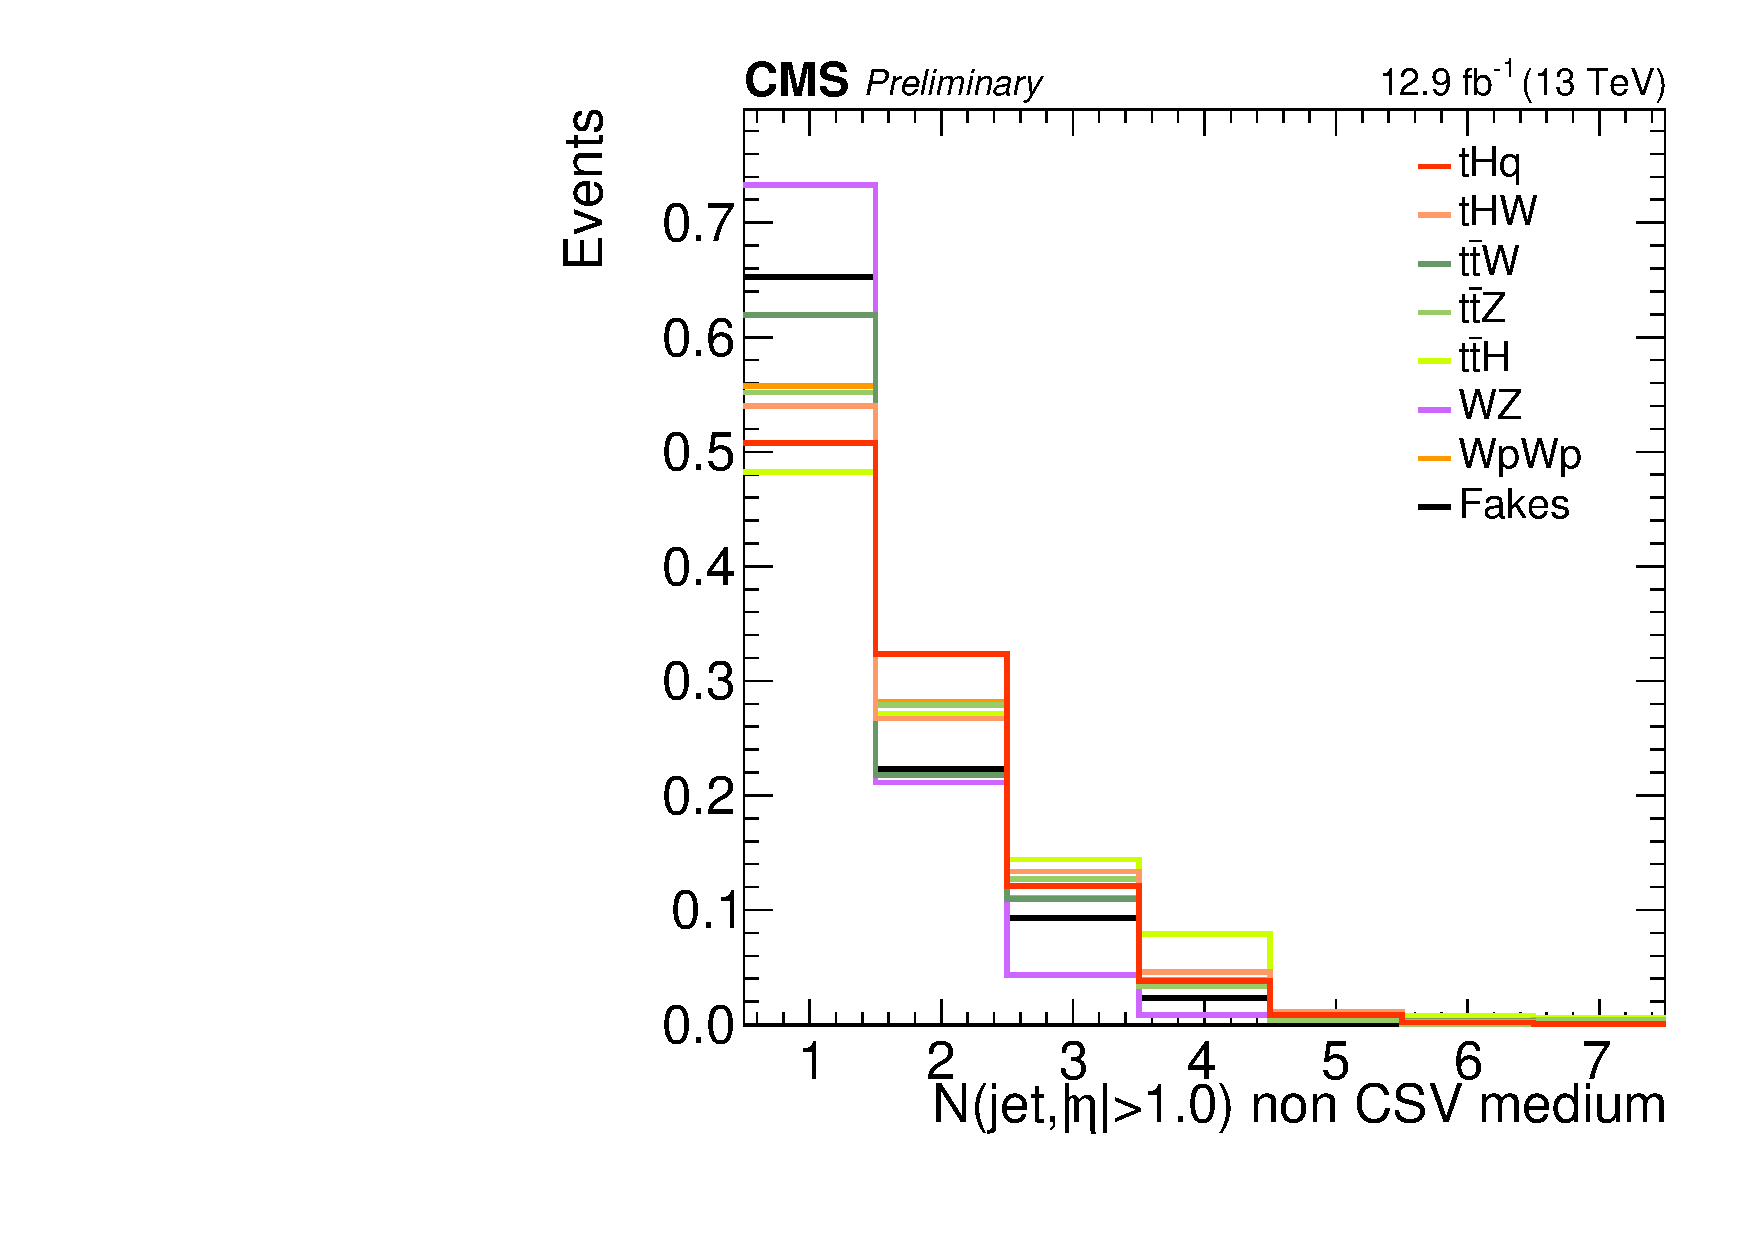
\includegraphics[width=0.245\textwidth]{figures/nJetEta1_mumu.pdf}
  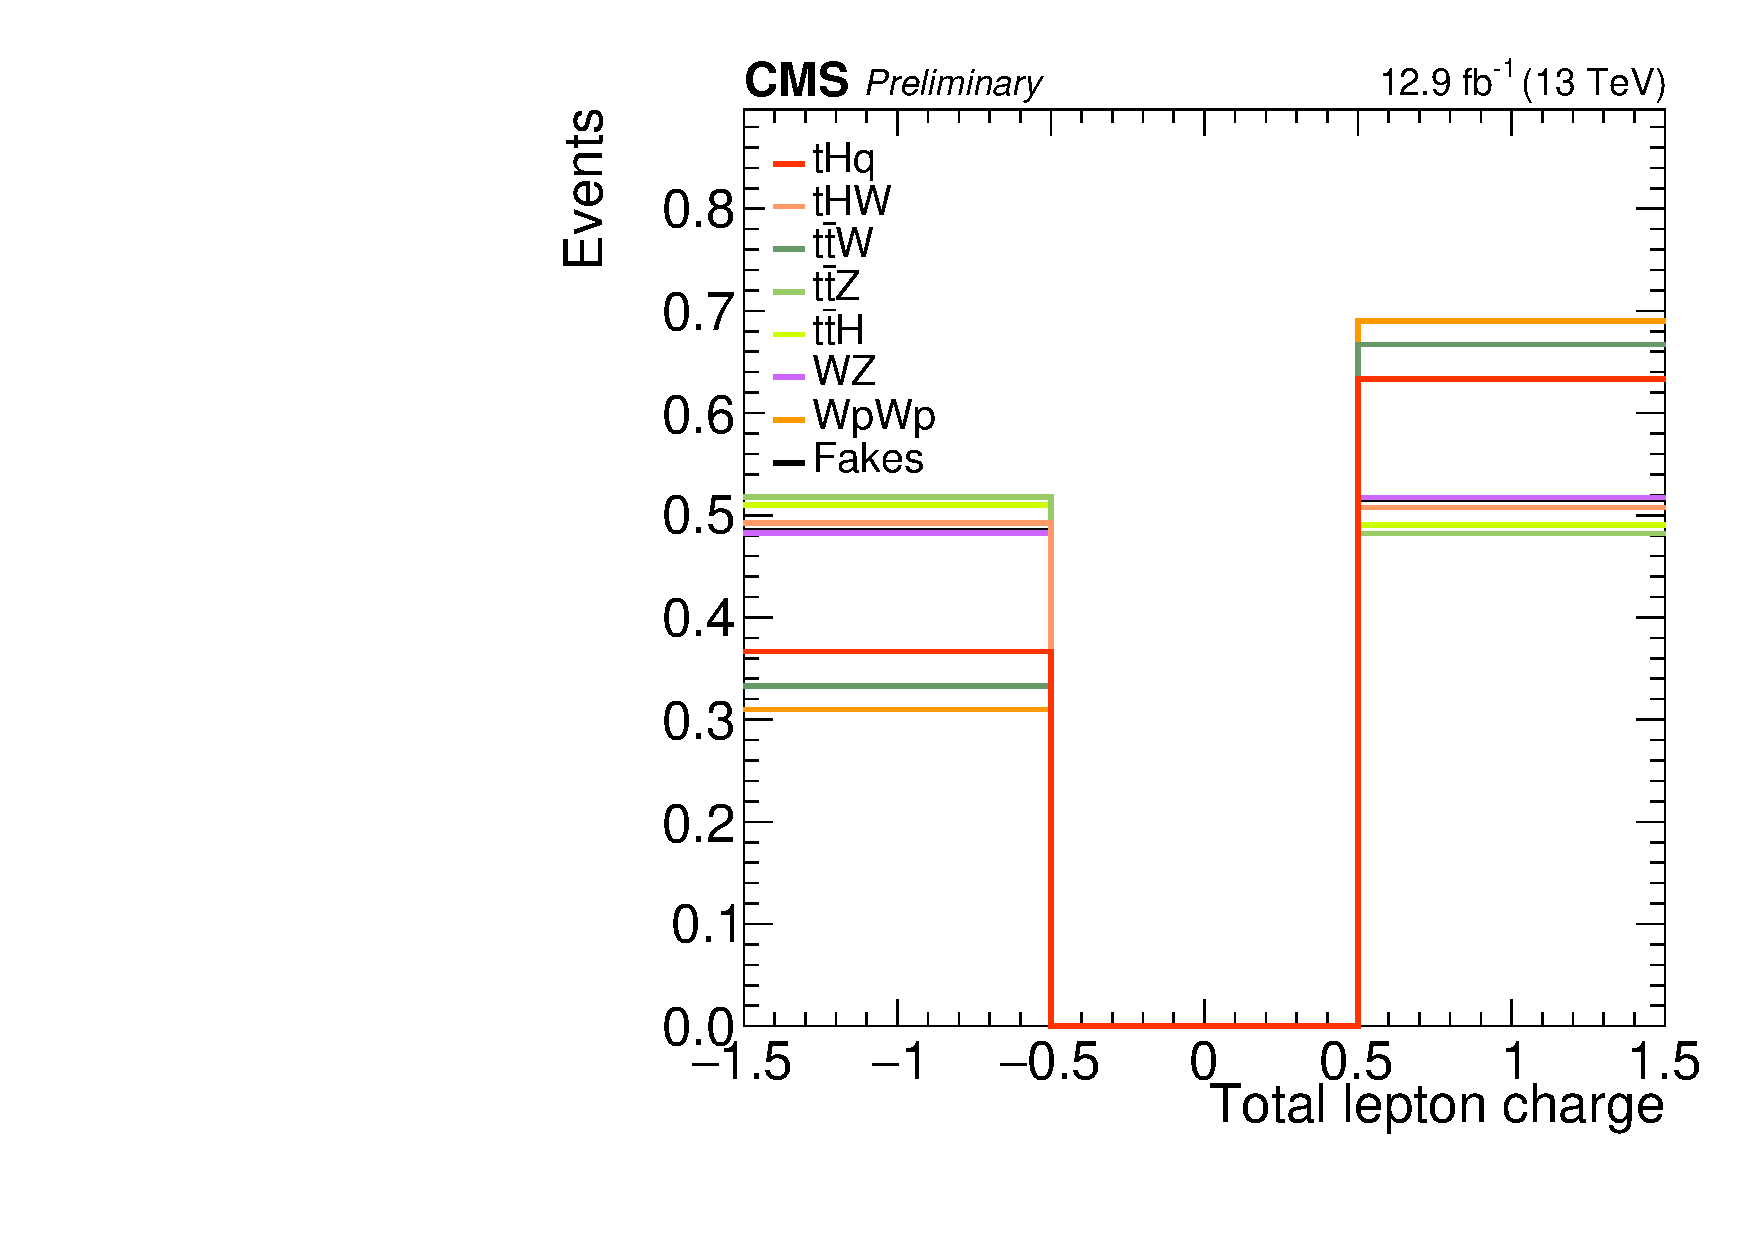
\includegraphics[width=0.245\textwidth]{figures/totCharge_mumu.pdf}
 \caption{Distributions of input variables to the BDT for signal discrimination, two lepton same sign channel.}
\label{fig:input_vars_2lss}
\end{figure}    

The MVA analysis consist of two stages: first a ``training'' where the MVA method is trained to discriminate between simulated signal and background events, then a ``test'' stage where the trained algorithm is used to classify different events from the samples.
The sample is obtained from a pre-selection (see Tab.~\ref{tab:evsel} with pre-selection cuts).

Figures~\ref{mva_input_tt} and~\ref{mva_input_ttv} show the input variables distributions as seen by the MVA algorithm.
Note that in contrast to the distributions in Fig.~\ref{fig:input_vars_3l} only the main backgrounds (\ttbar\ from simulation, \ttV) are included.

\begin{figure} [!h]
  \centering
  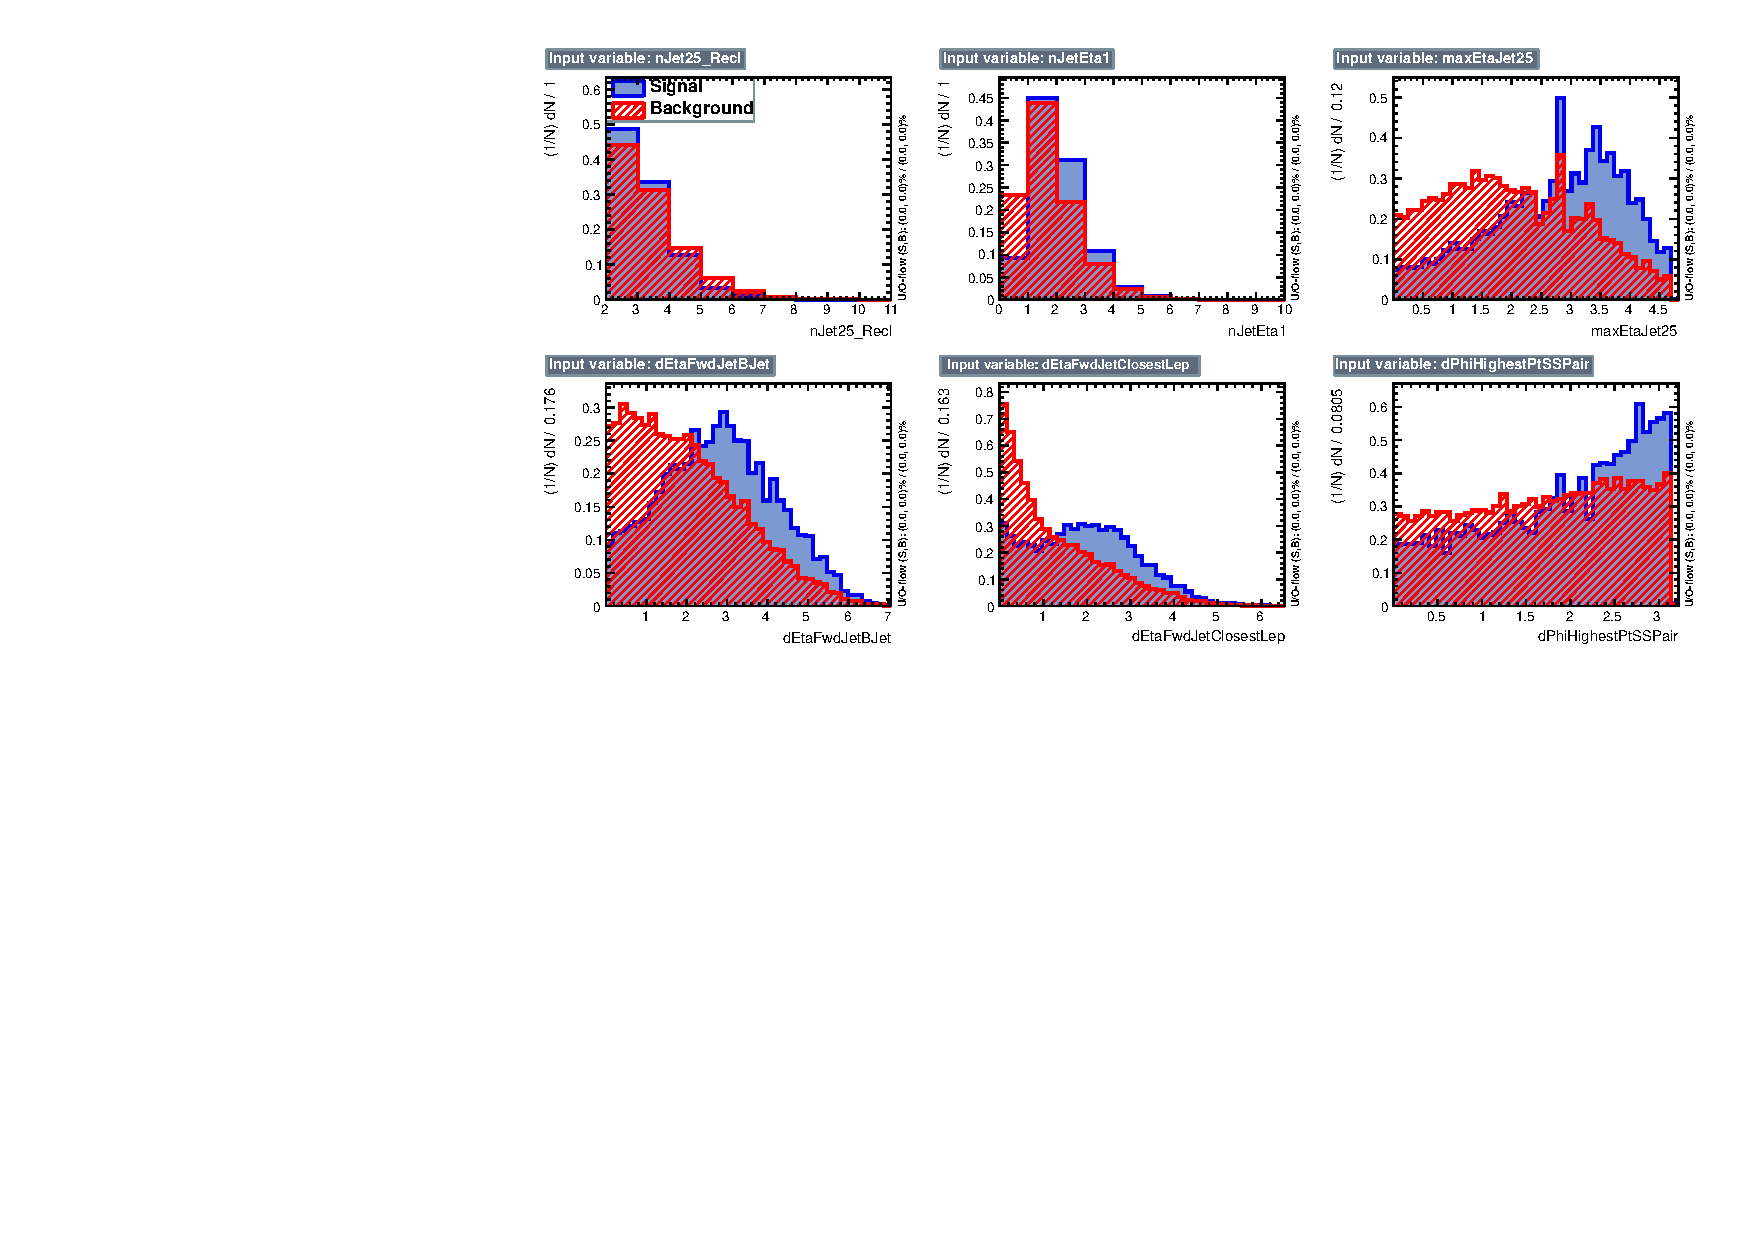
\includegraphics[width=\textwidth]{figures/mva_input1_tt.pdf}
  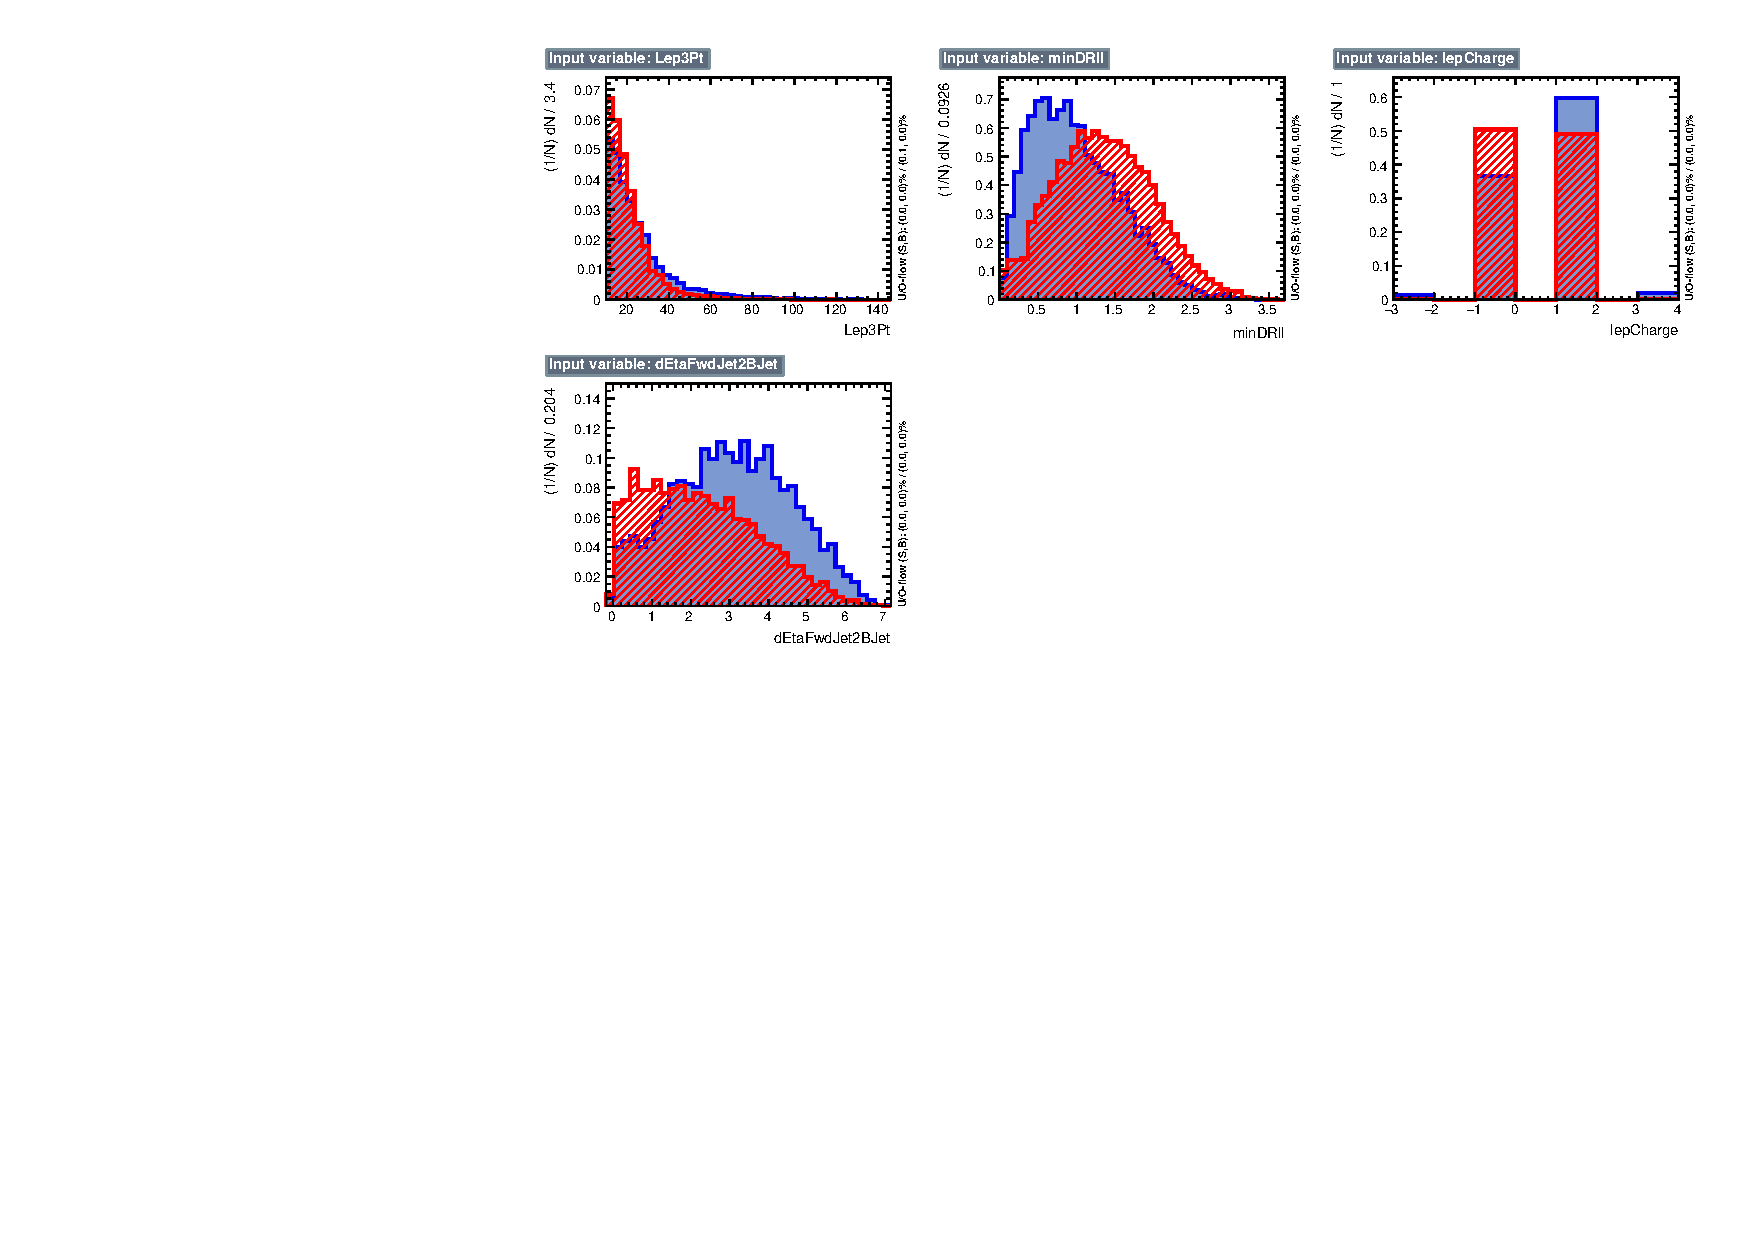
\includegraphics[width=\textwidth]{figures/mva_input2_tt.pdf}
\caption{BDT inputs as seen by TMVA (signal, in blue, is \tHq, background, in red, is \ttbar) for the three lepton channel, discriminated against \ttbar\ (fakes) background.} 
\label{mva_input_tt}
\end{figure}

\begin{figure} [!h]
  \centering
  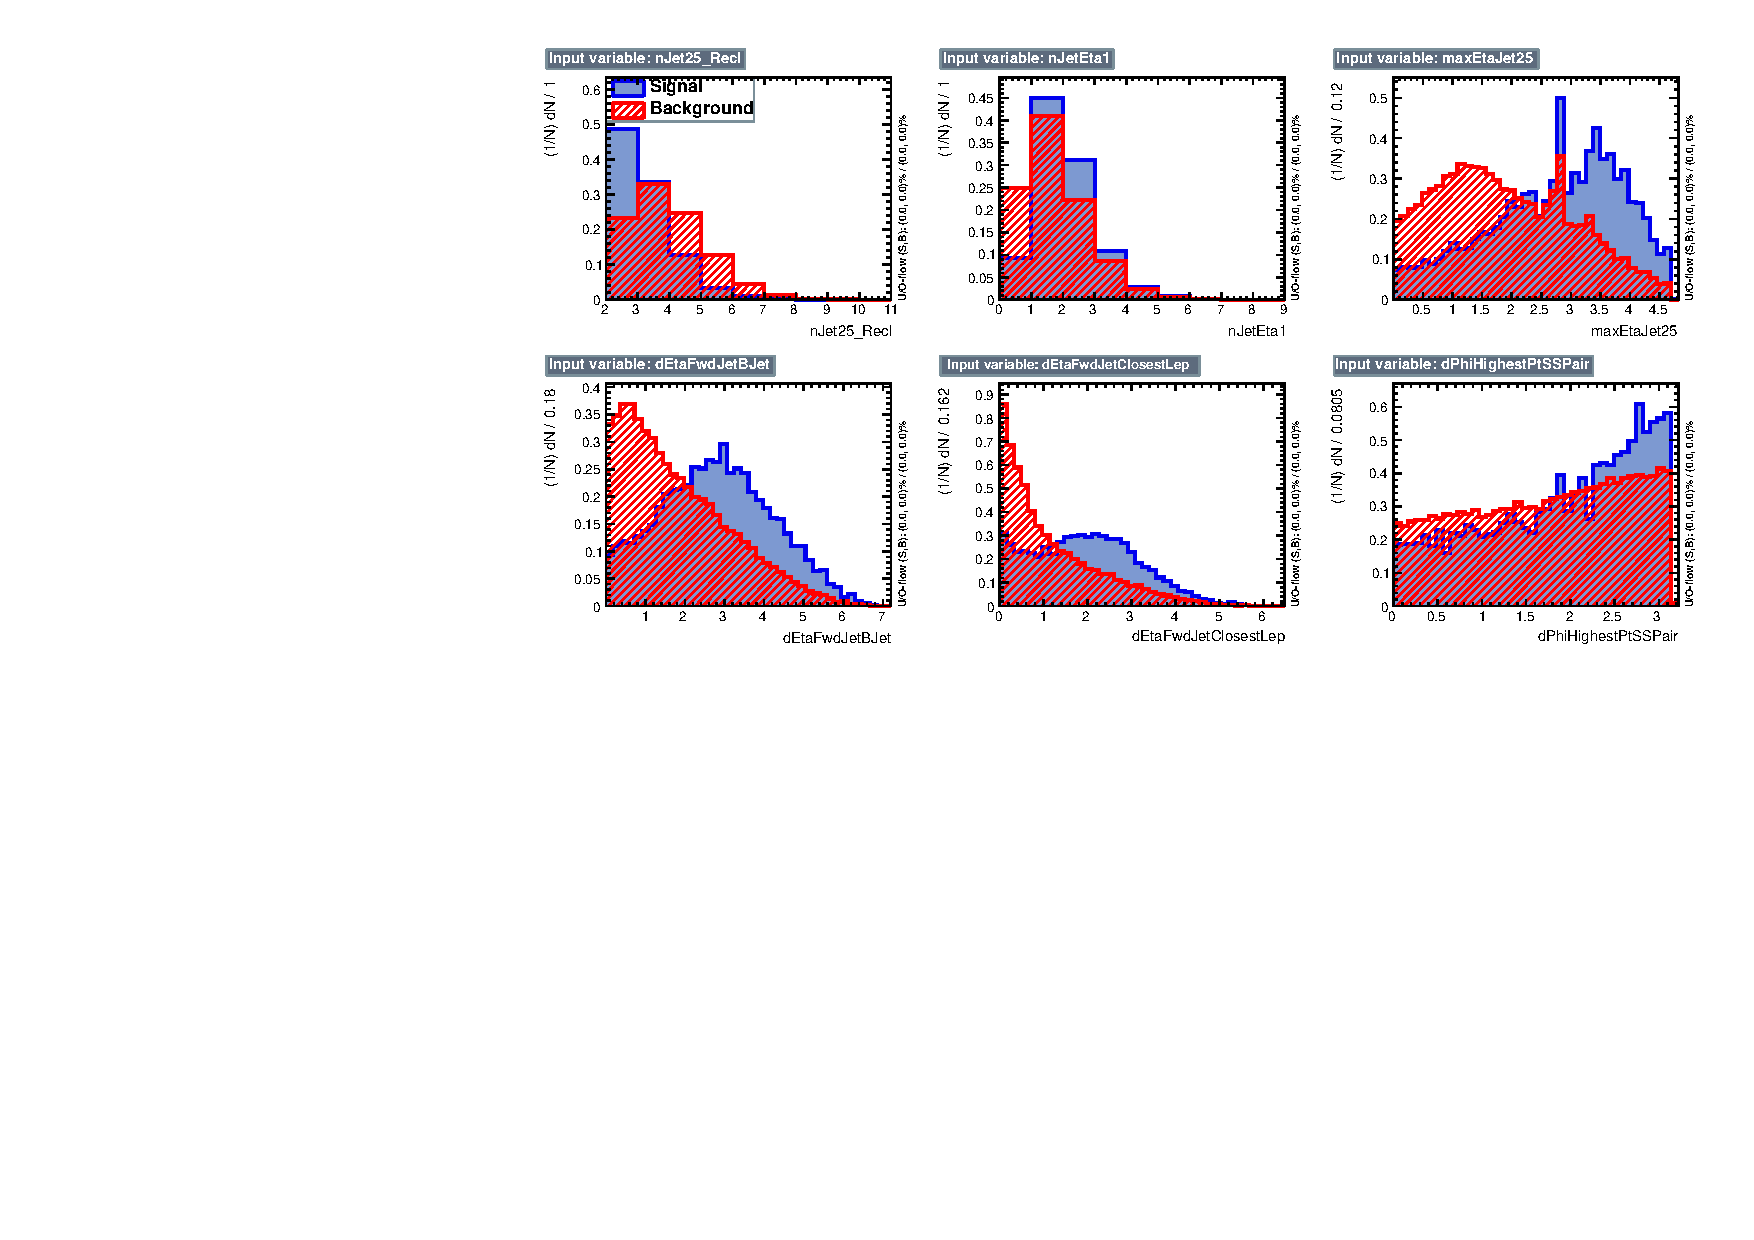
\includegraphics[width=\textwidth]{figures/mva_input1_ttv.pdf}
  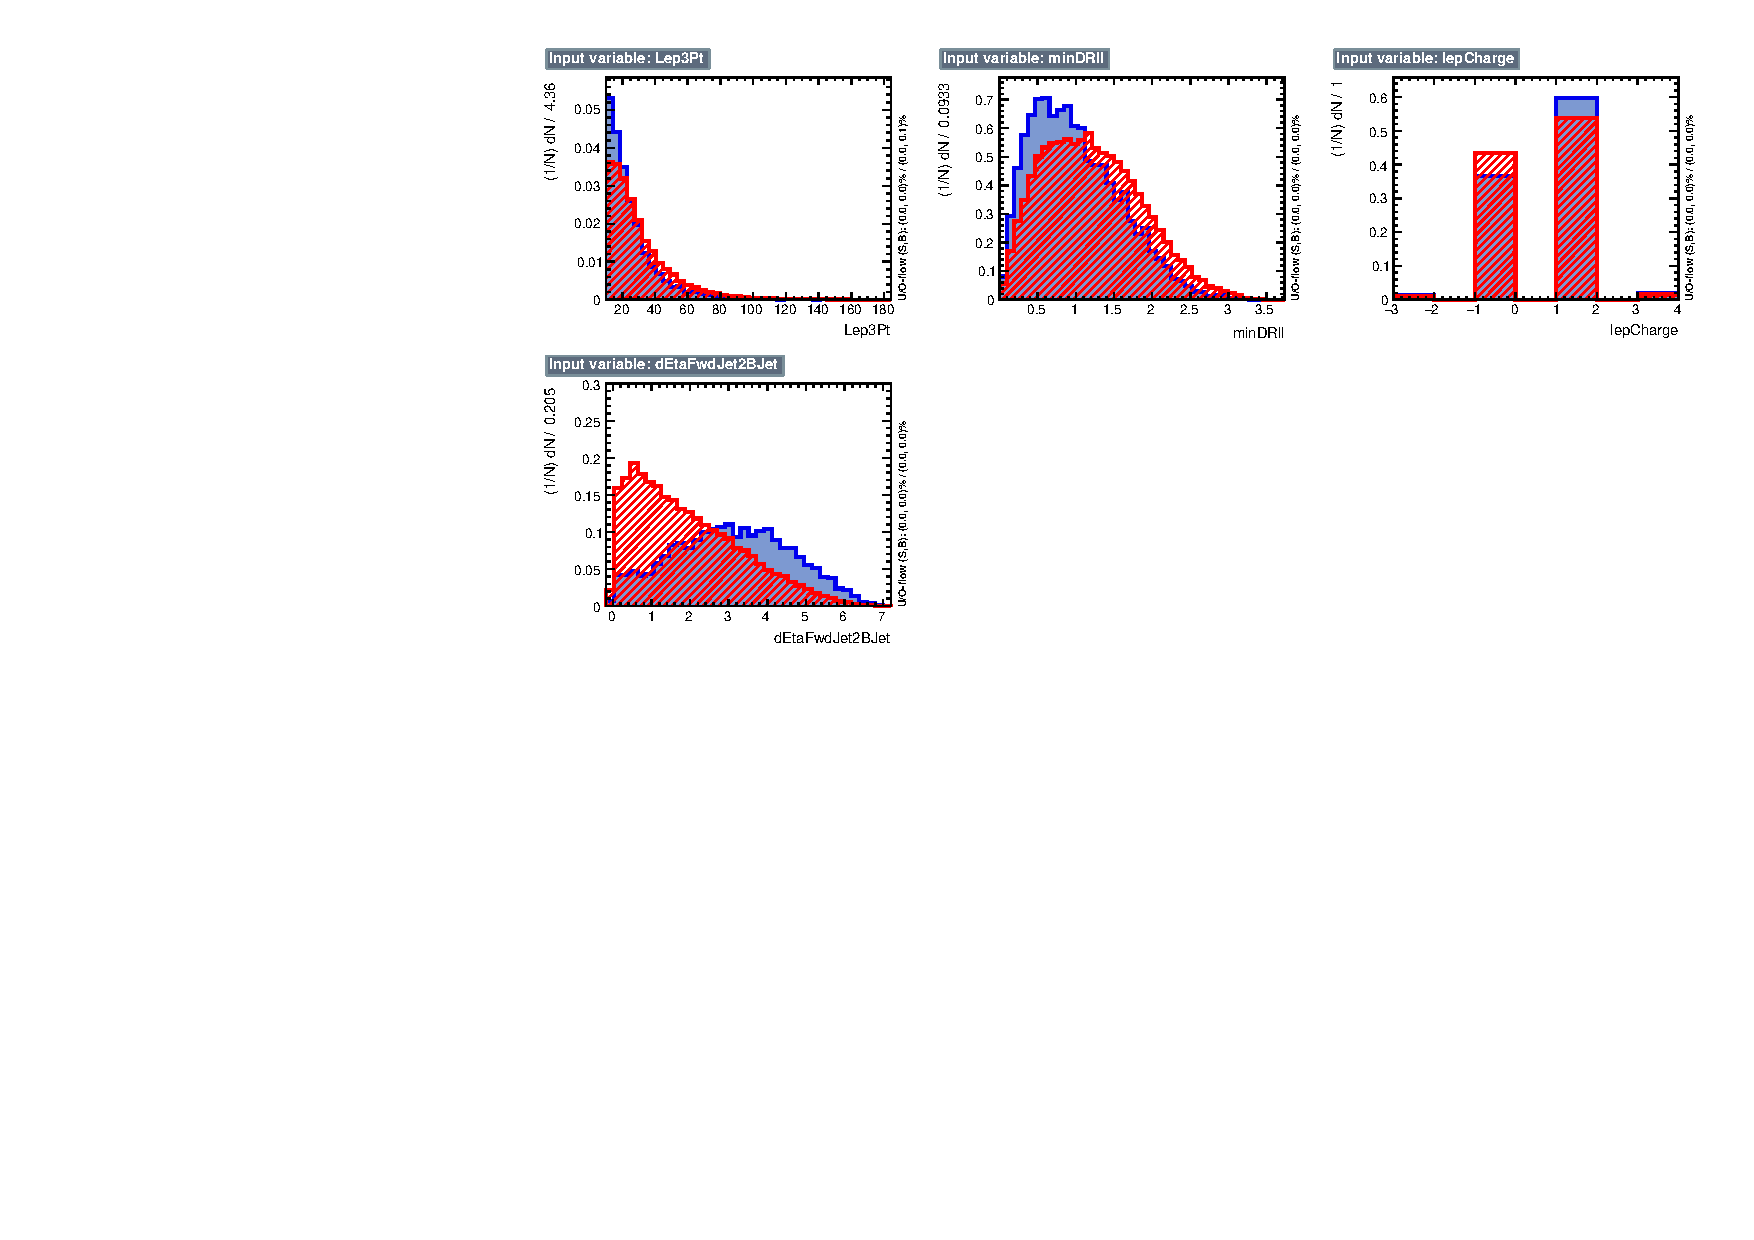
\includegraphics[width=\textwidth]{figures/mva_input2_ttv.pdf}
\caption{BDT inputs as seen by TMVA (signal, in blue, is \tHq, background, in red, is \ttW+\ttZ) for the three lepton channel, discriminated against \ttV\ background.}                                                                                                                                                         
\label{mva_input_ttv}
\end{figure}

The input variables distributions for 2lss channel for signal against the \ttbar\ and \ttV\ are shown in Figure~\ref{mva_input_2lss_tt} and Figure~\ref{mva_input_2lss_ttv} respectively.
\begin{figure} [!h]
  \centering
  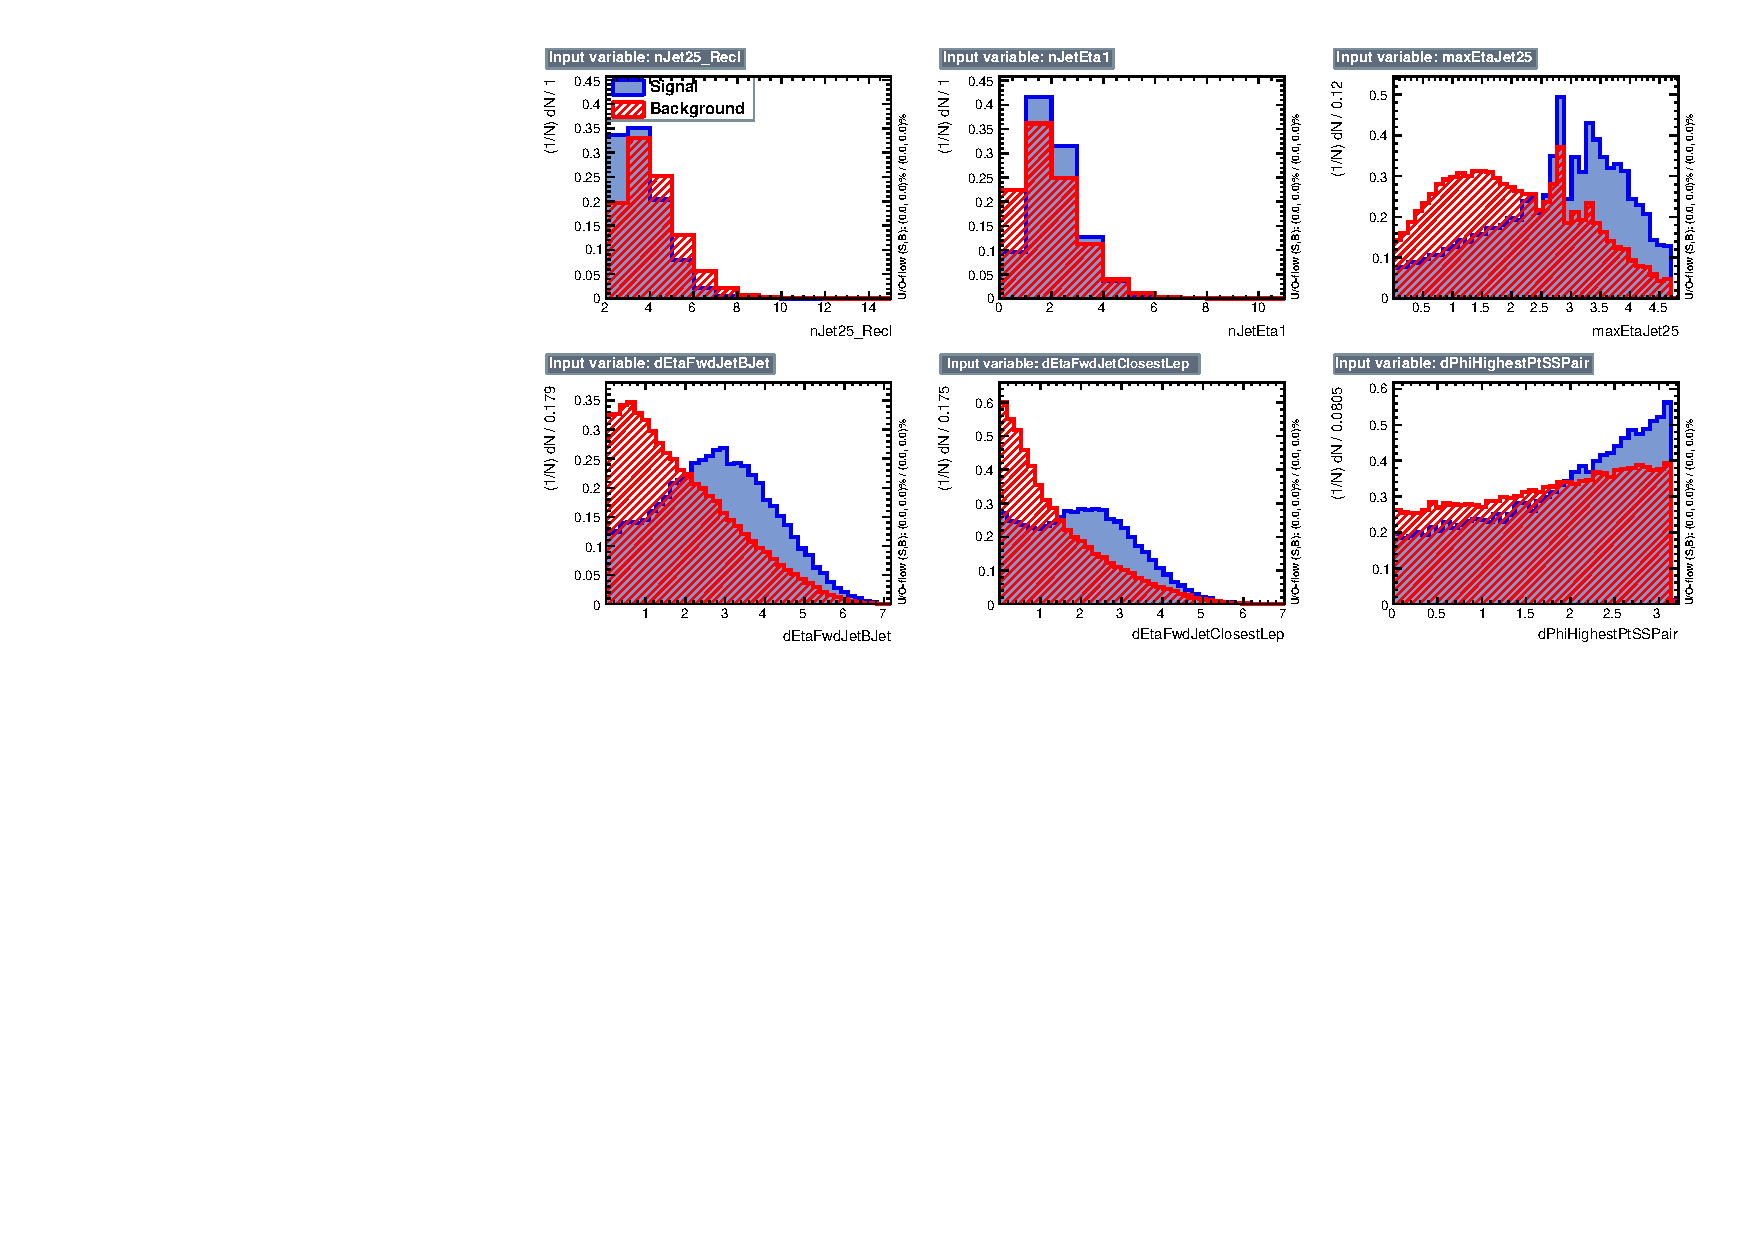
\includegraphics[width=\textwidth]{figures/6var_tt.pdf}
  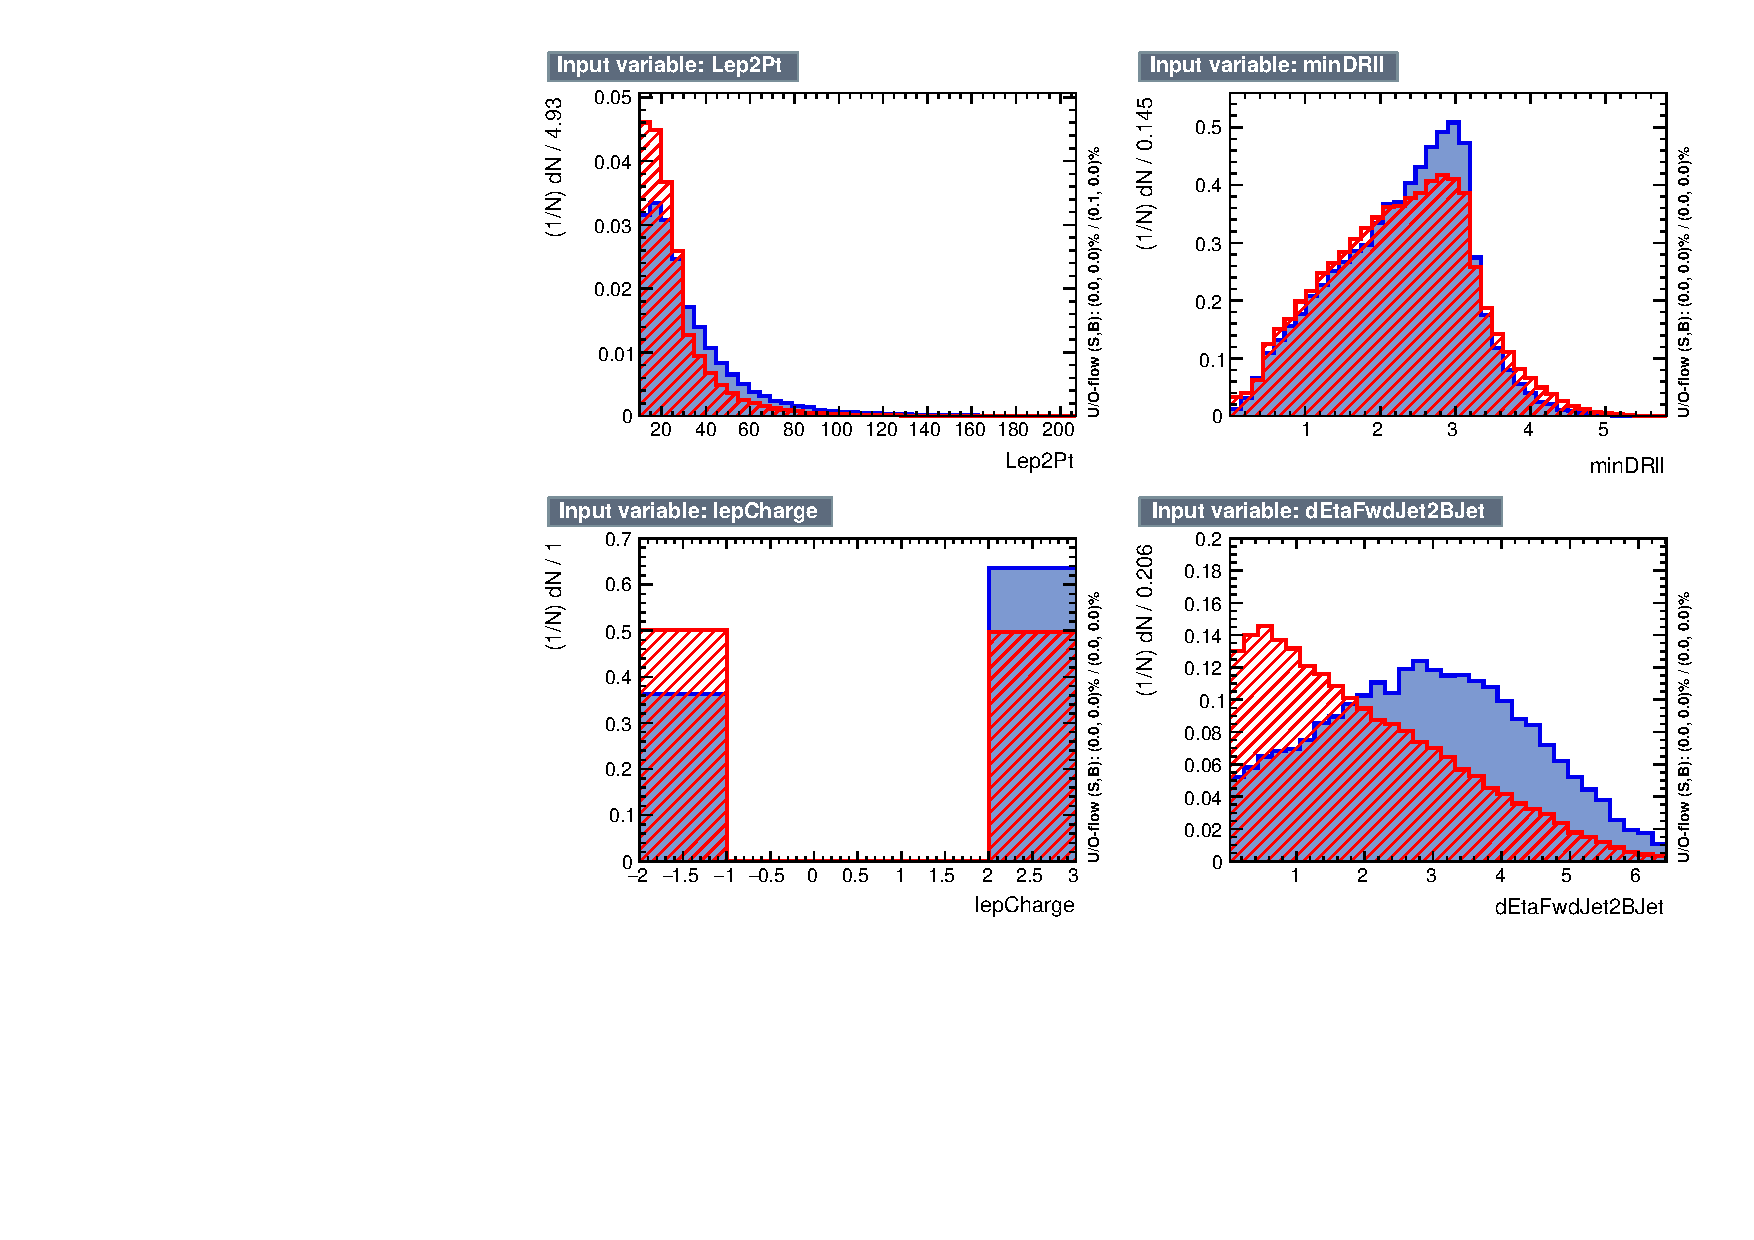
\includegraphics[width=0.66\textwidth]{figures/4var_tt.pdf}
\caption{BDT inputs as seen by TMVA (signal, in blue, is \tHq, background, in red, is \ttbar) for the same sign dilepton channel, discriminated against \ttbar\ background.} 
\label{mva_input_2lss_tt}
\end{figure}

\begin{figure} [!h]
  \centering
  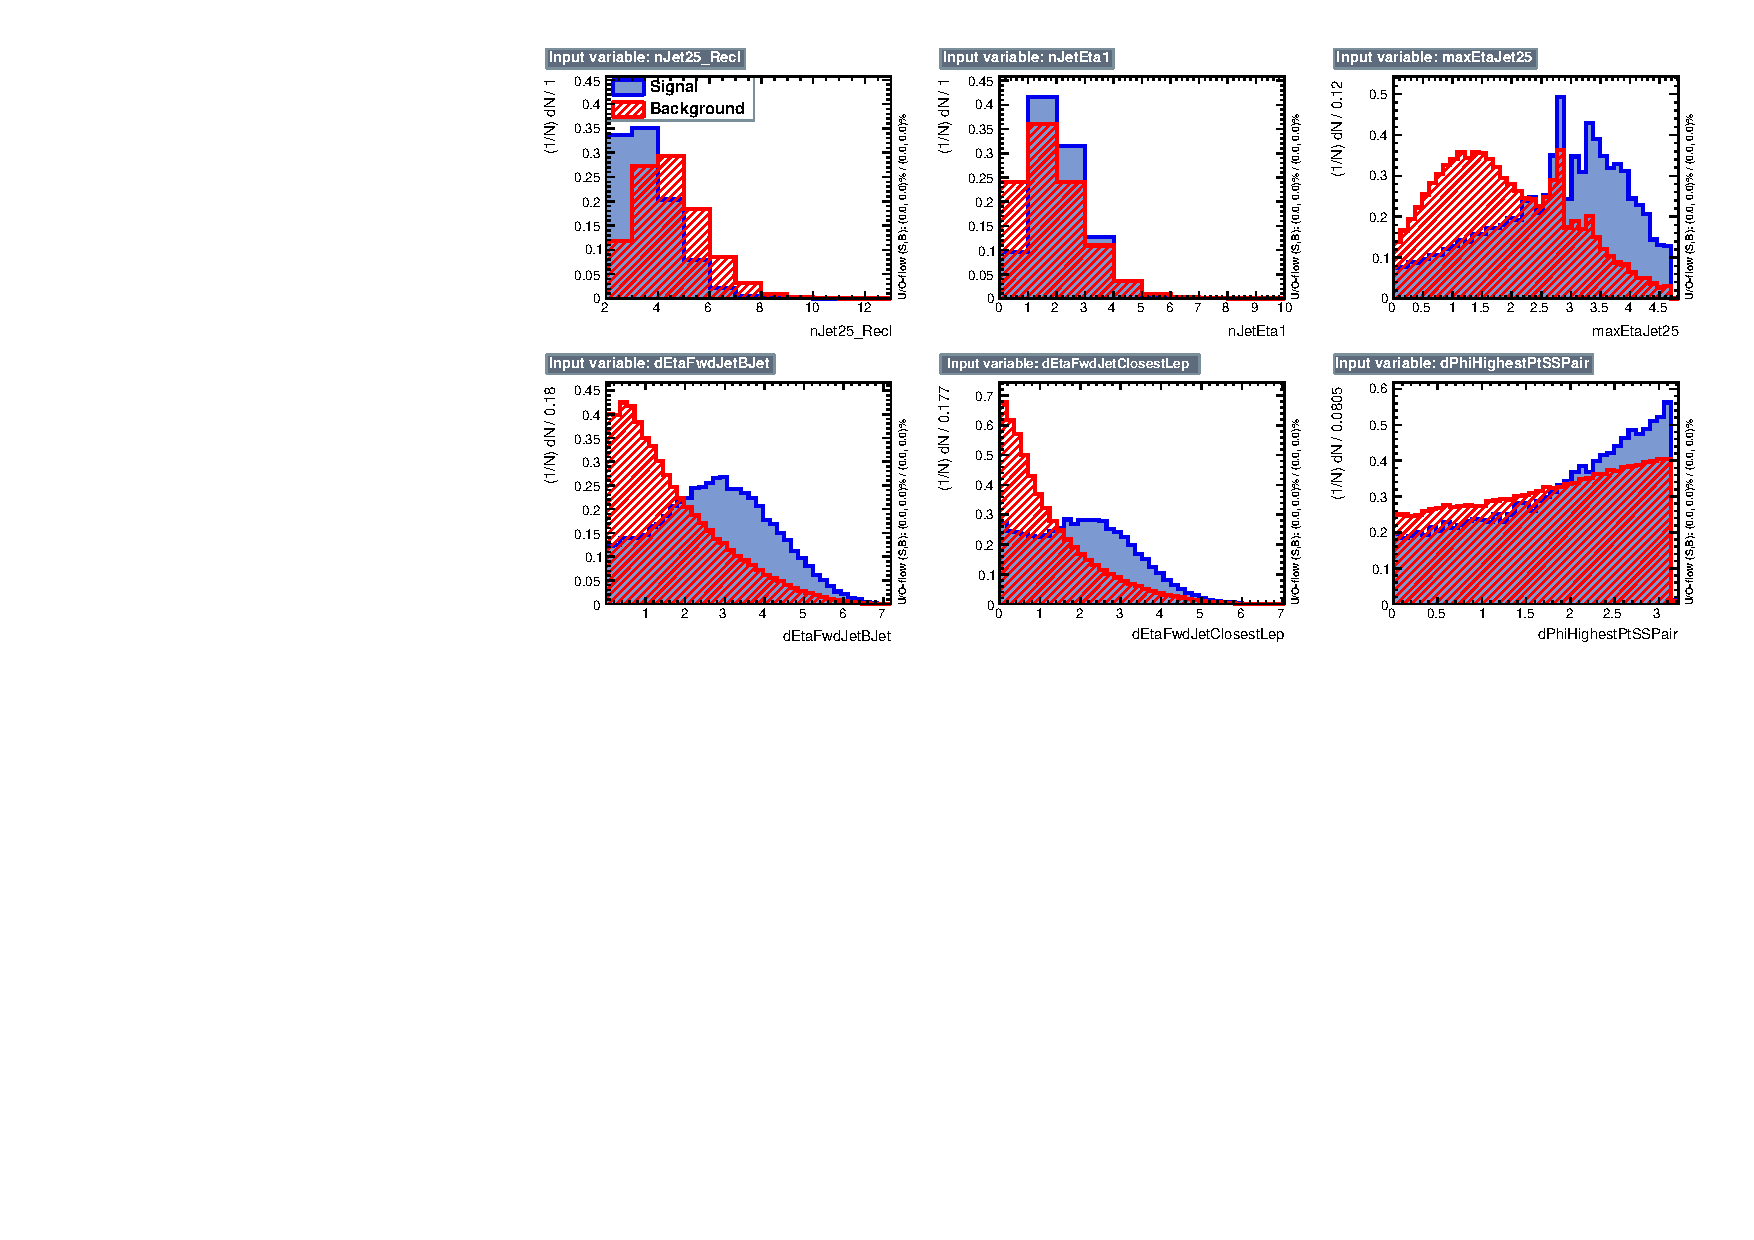
\includegraphics[width=\textwidth]{figures/6var_ttv.pdf}
  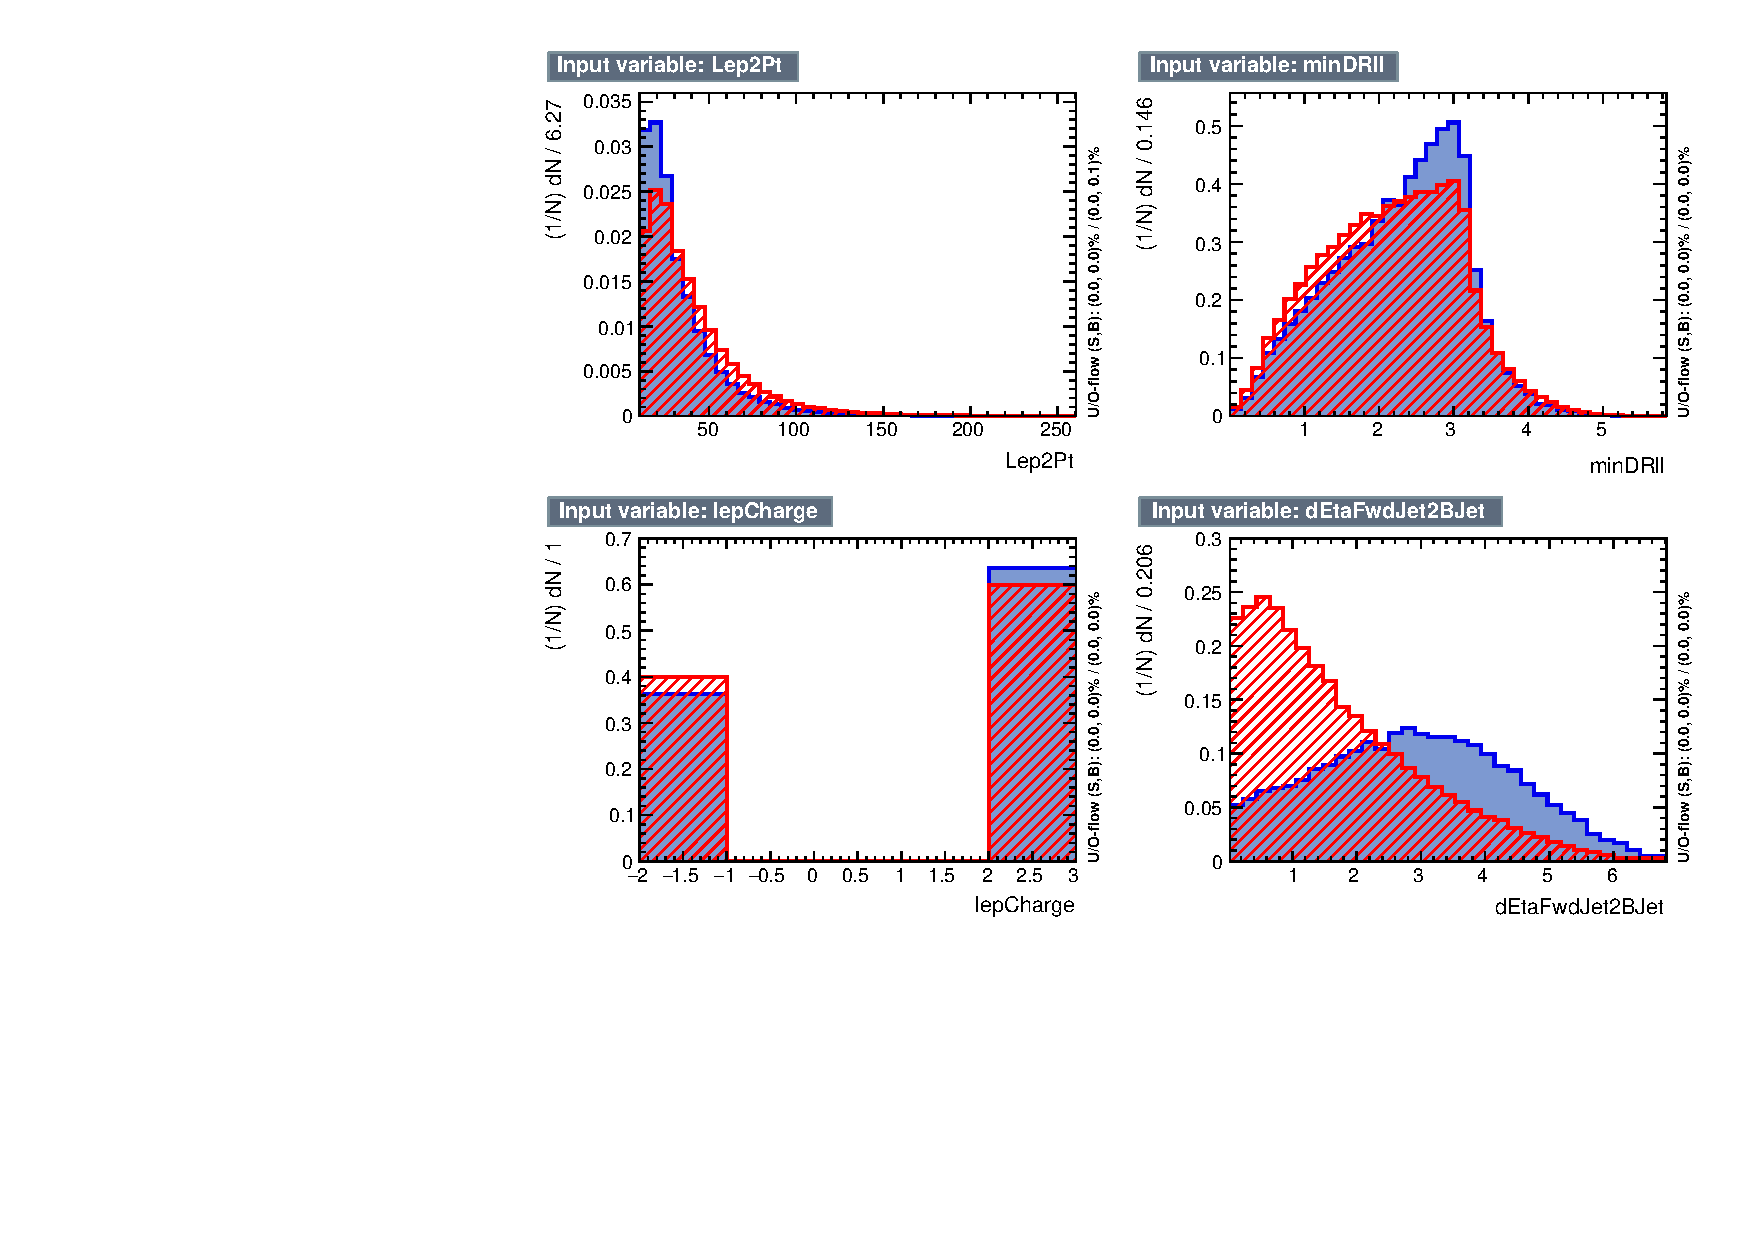
\includegraphics[width=0.66\textwidth]{figures/4var_ttv.pdf}
\caption{BDT inputs as seen by TMVA (signal, in blue, is \tHq, background, in red, is \ttW+\ttZ) for the same sign dilepton channel, discriminated against \ttV\ background.}
\label{mva_input_2lss_ttv}
\end{figure}

Note that splitting the training in two groups reveals that some variables show opposite behavior for the two background sources; potentially screening the discrimination power if they were to be used in a single discriminant.
For some other variables the distributions are similar in both background cases.

From table~\ref{tab:bdtinputs}, it is clear that the input variables are correlated to some extend. These correlations play an important role for some MVA methods like the Fisher discriminant method in which the first step consist of performing a linear transformation to an phase space where the correlations between variables are removed. In case a boosted decision tree (BDT) method however, correlations do not affect the performance.

Figure~\ref{mva_corr} show the linear correlation coefficients for signal and background for the two training cases (the signal values are identical by construction). As expected, strong correlations appears for variables related to the forward jet activity. Same trend is seen in case of the same sign dilepton channel in Figure~\ref{mva_corr_2lss}.

\begin{figure} [!h]
  \centering
   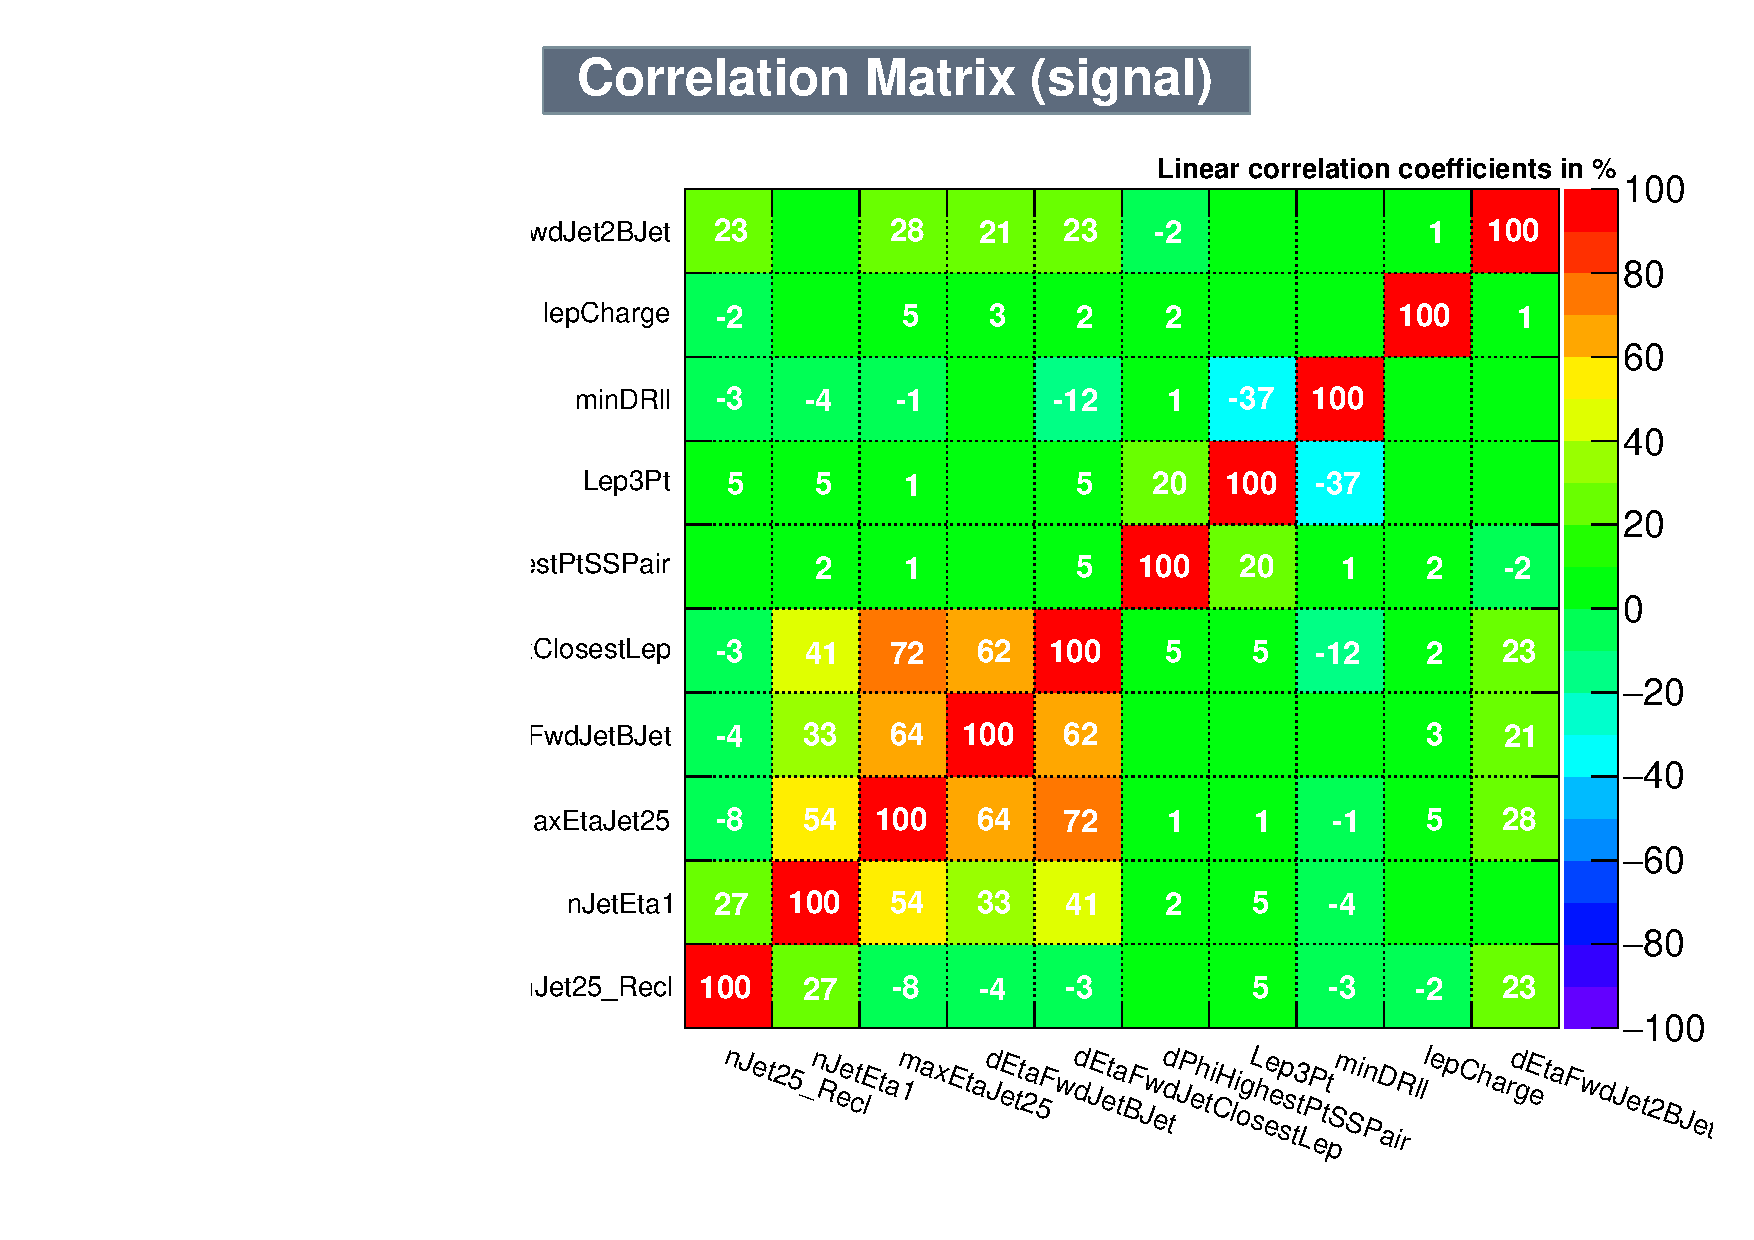
\includegraphics[width=0.32\textwidth]{figures/corr_signal.pdf}
   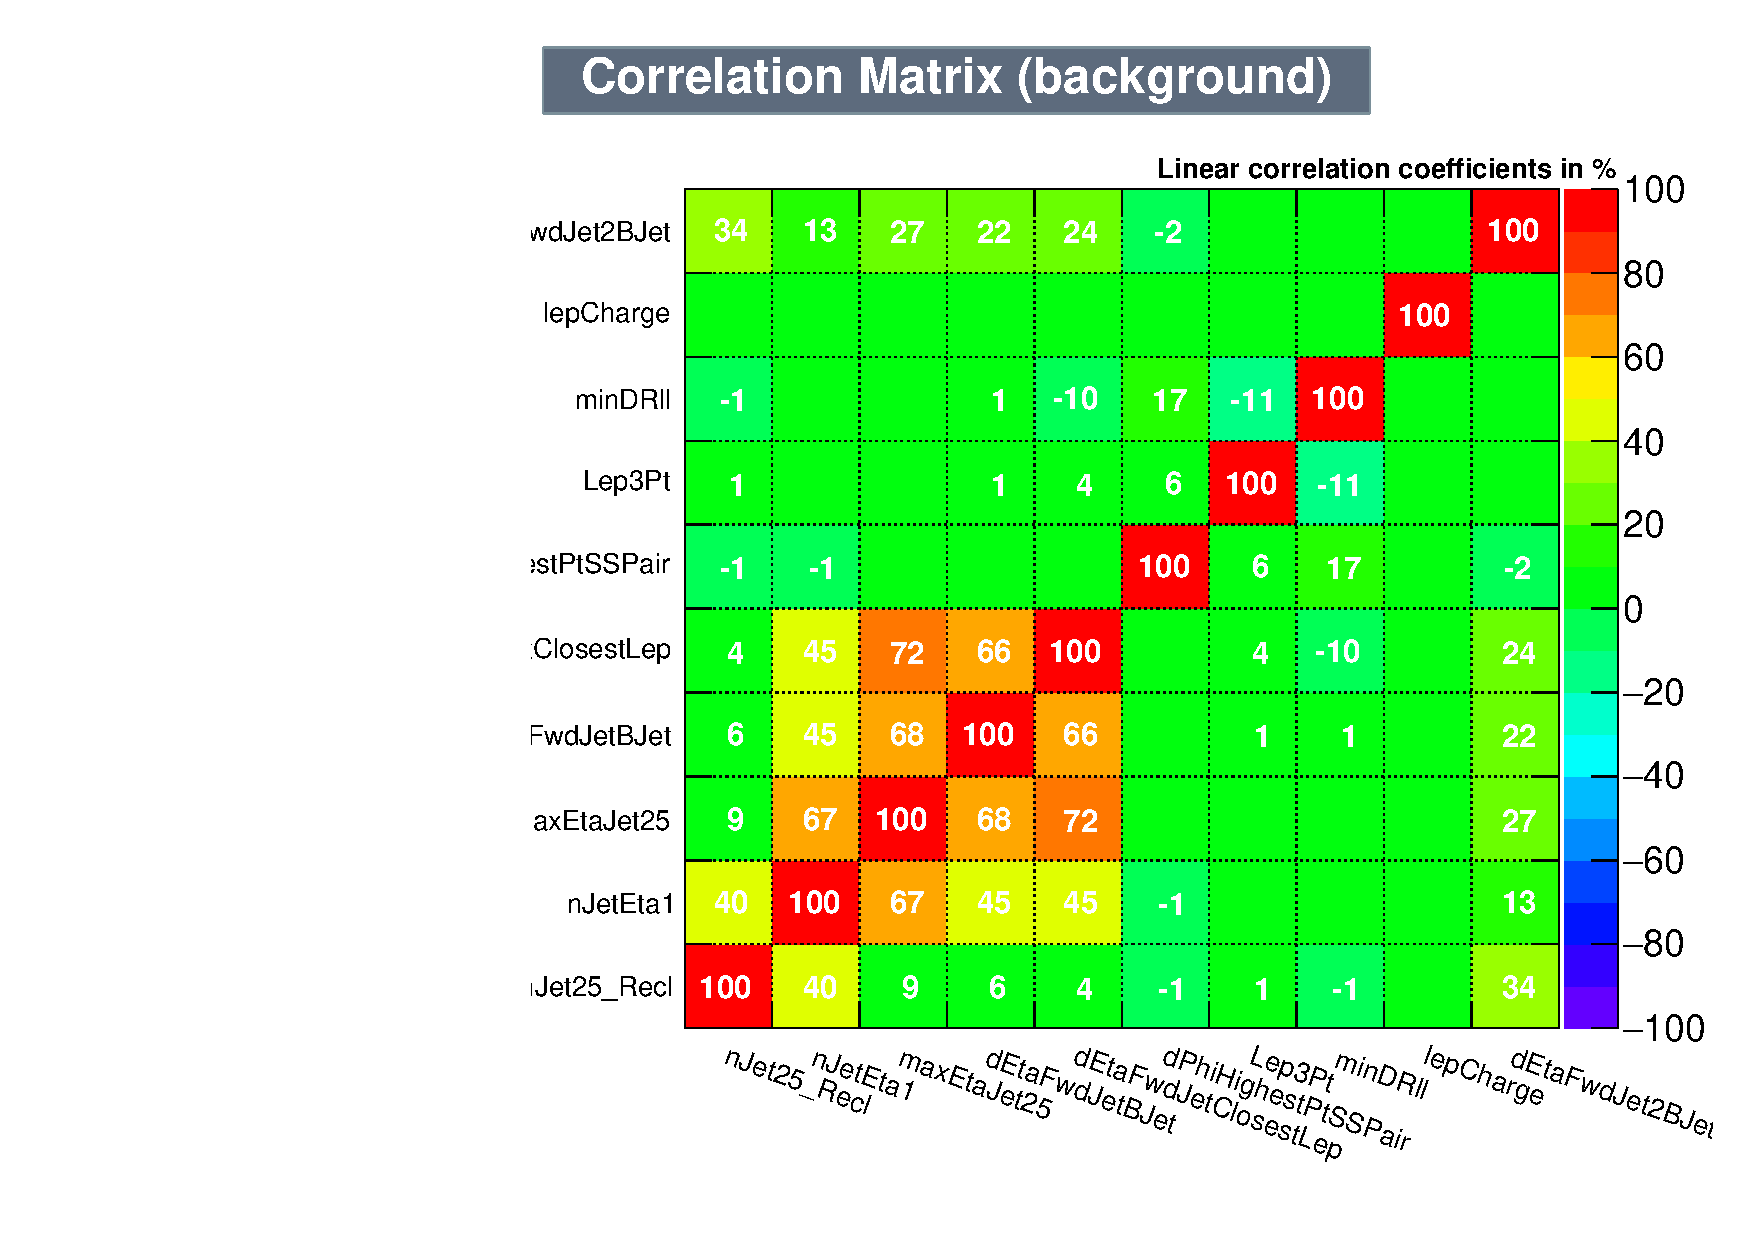
\includegraphics[width=0.32\textwidth]{figures/corr_tt.pdf}
   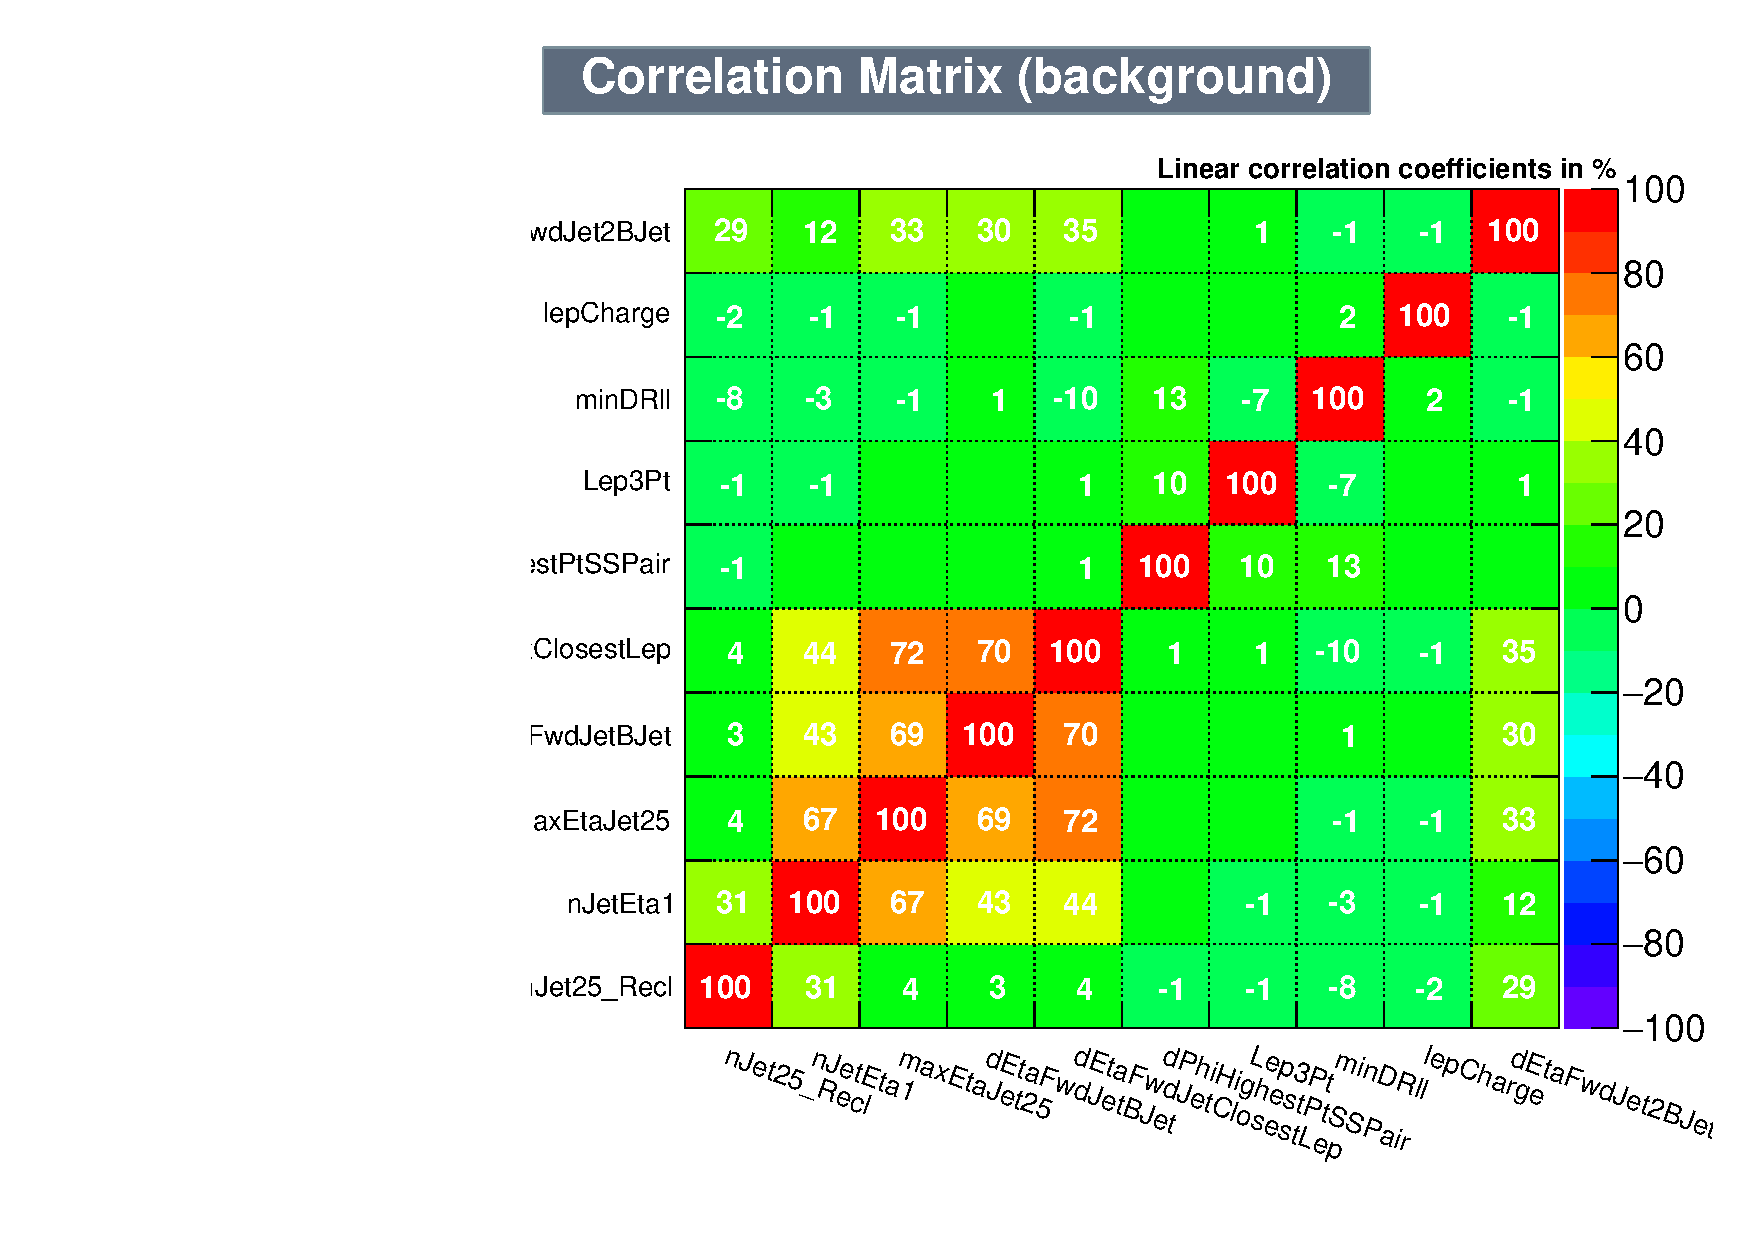
\includegraphics[width=0.32\textwidth]{figures/corr_ttv.pdf}

\caption{ Signal (left), \ttbar\ background (middle), and \ttV\ background (right.) correlation matrices for the input variables in the TMVA analysis for the three lepton channel.}
\label{mva_corr}
\end{figure}

\begin{figure} [!h]
  \centering
  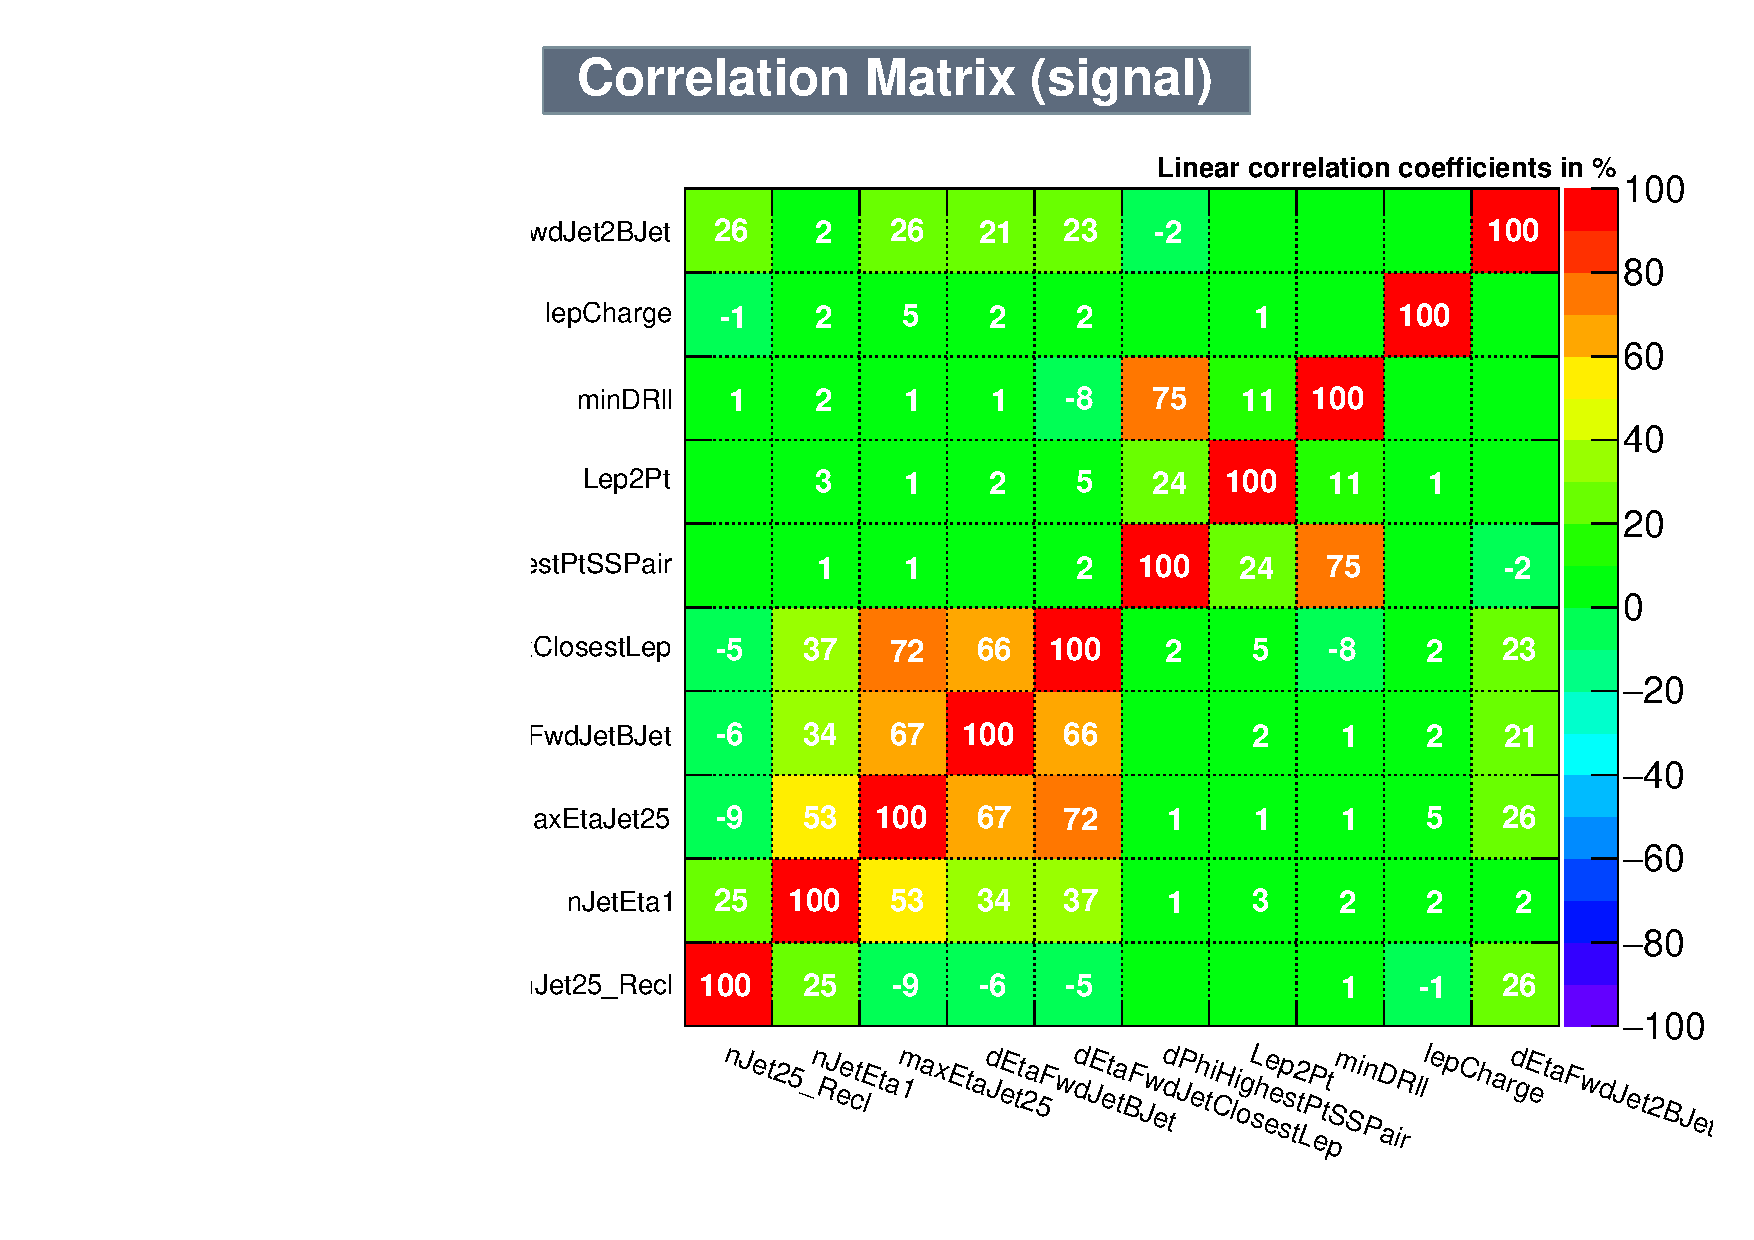
\includegraphics[width=0.32\textwidth]{figures/sig_corr_tt_2lss.pdf}
  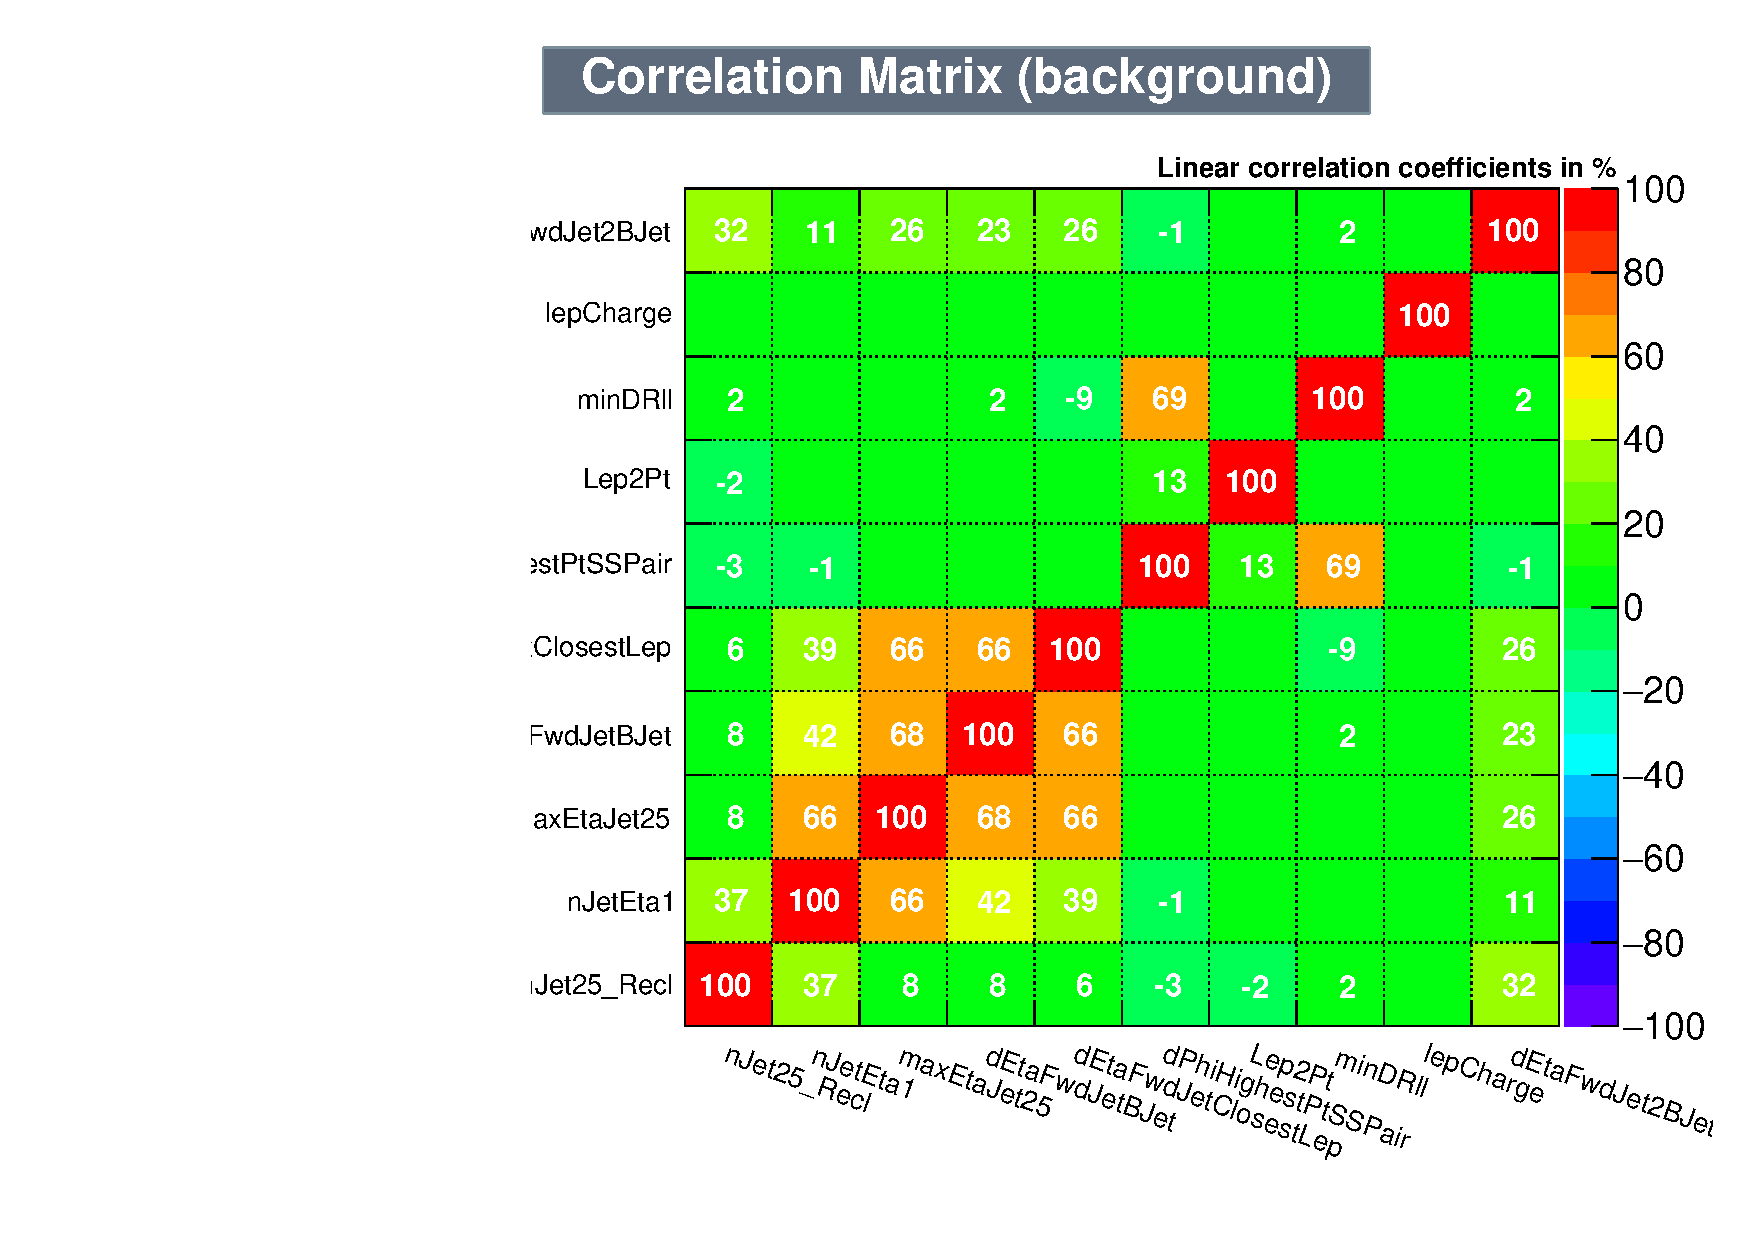
\includegraphics[width=0.32\textwidth]{figures/bkg_corr_tt_2lss.pdf}
  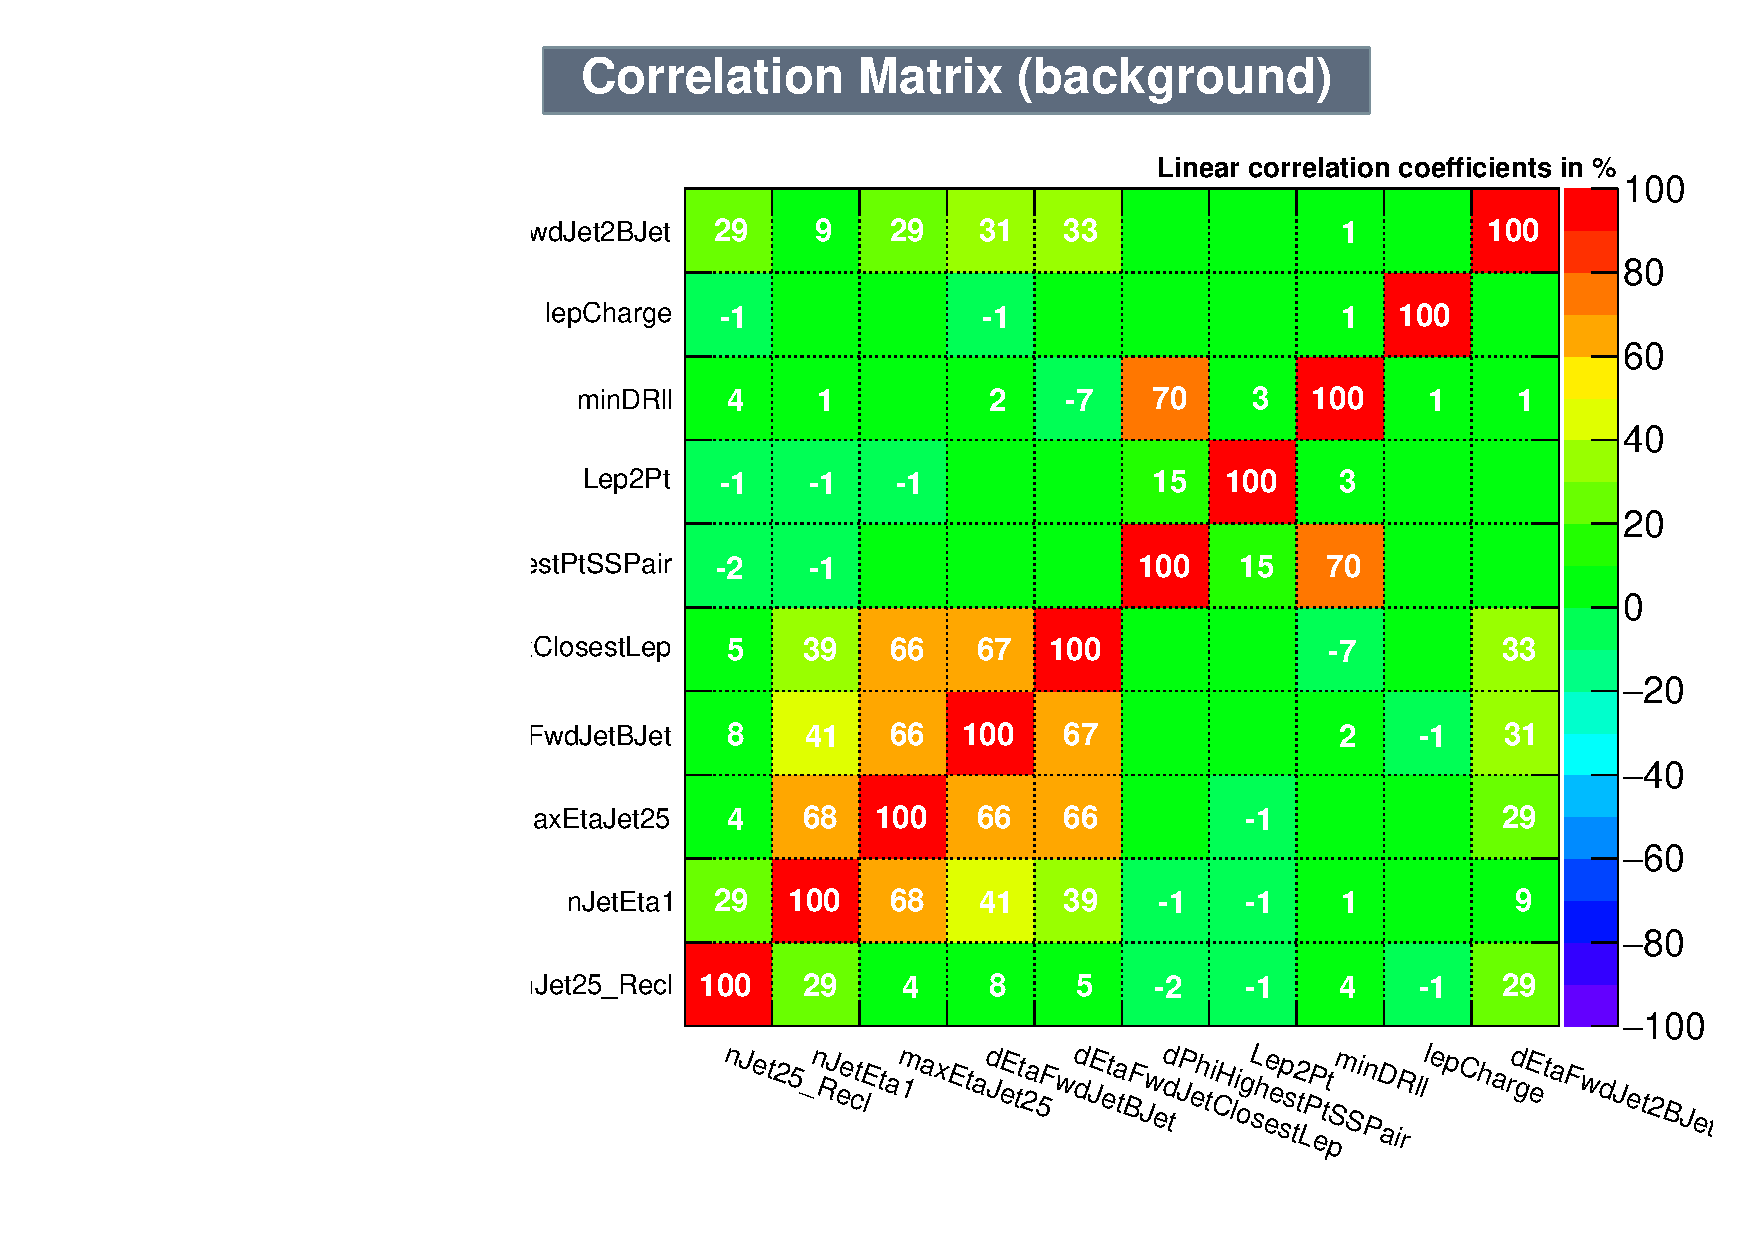
\includegraphics[width=0.32\textwidth]{figures/bkg_corr_ttv_2lss.pdf}
\caption{Signal and Background correlation matrices for the input variables in the TMVA analysis for the same sign dilepton channel, for the signal (left), \ttbar\ background (middle), and \ttV\ background (right.)}
\label{mva_corr_2lss}
\end{figure}

\subsection{Classifiers response}
Several MVA algorithms were evaluated to determine the most appropriate method for this analysis.
The plots in Fig.~\ref{roc} (top) show the background rejection as a function of the signal efficiency for \ttbar\ and \ttV\ trainings (ROC curves) for the different algorithms that were evaluated.

\begin{figure} [!h]
  \centering
   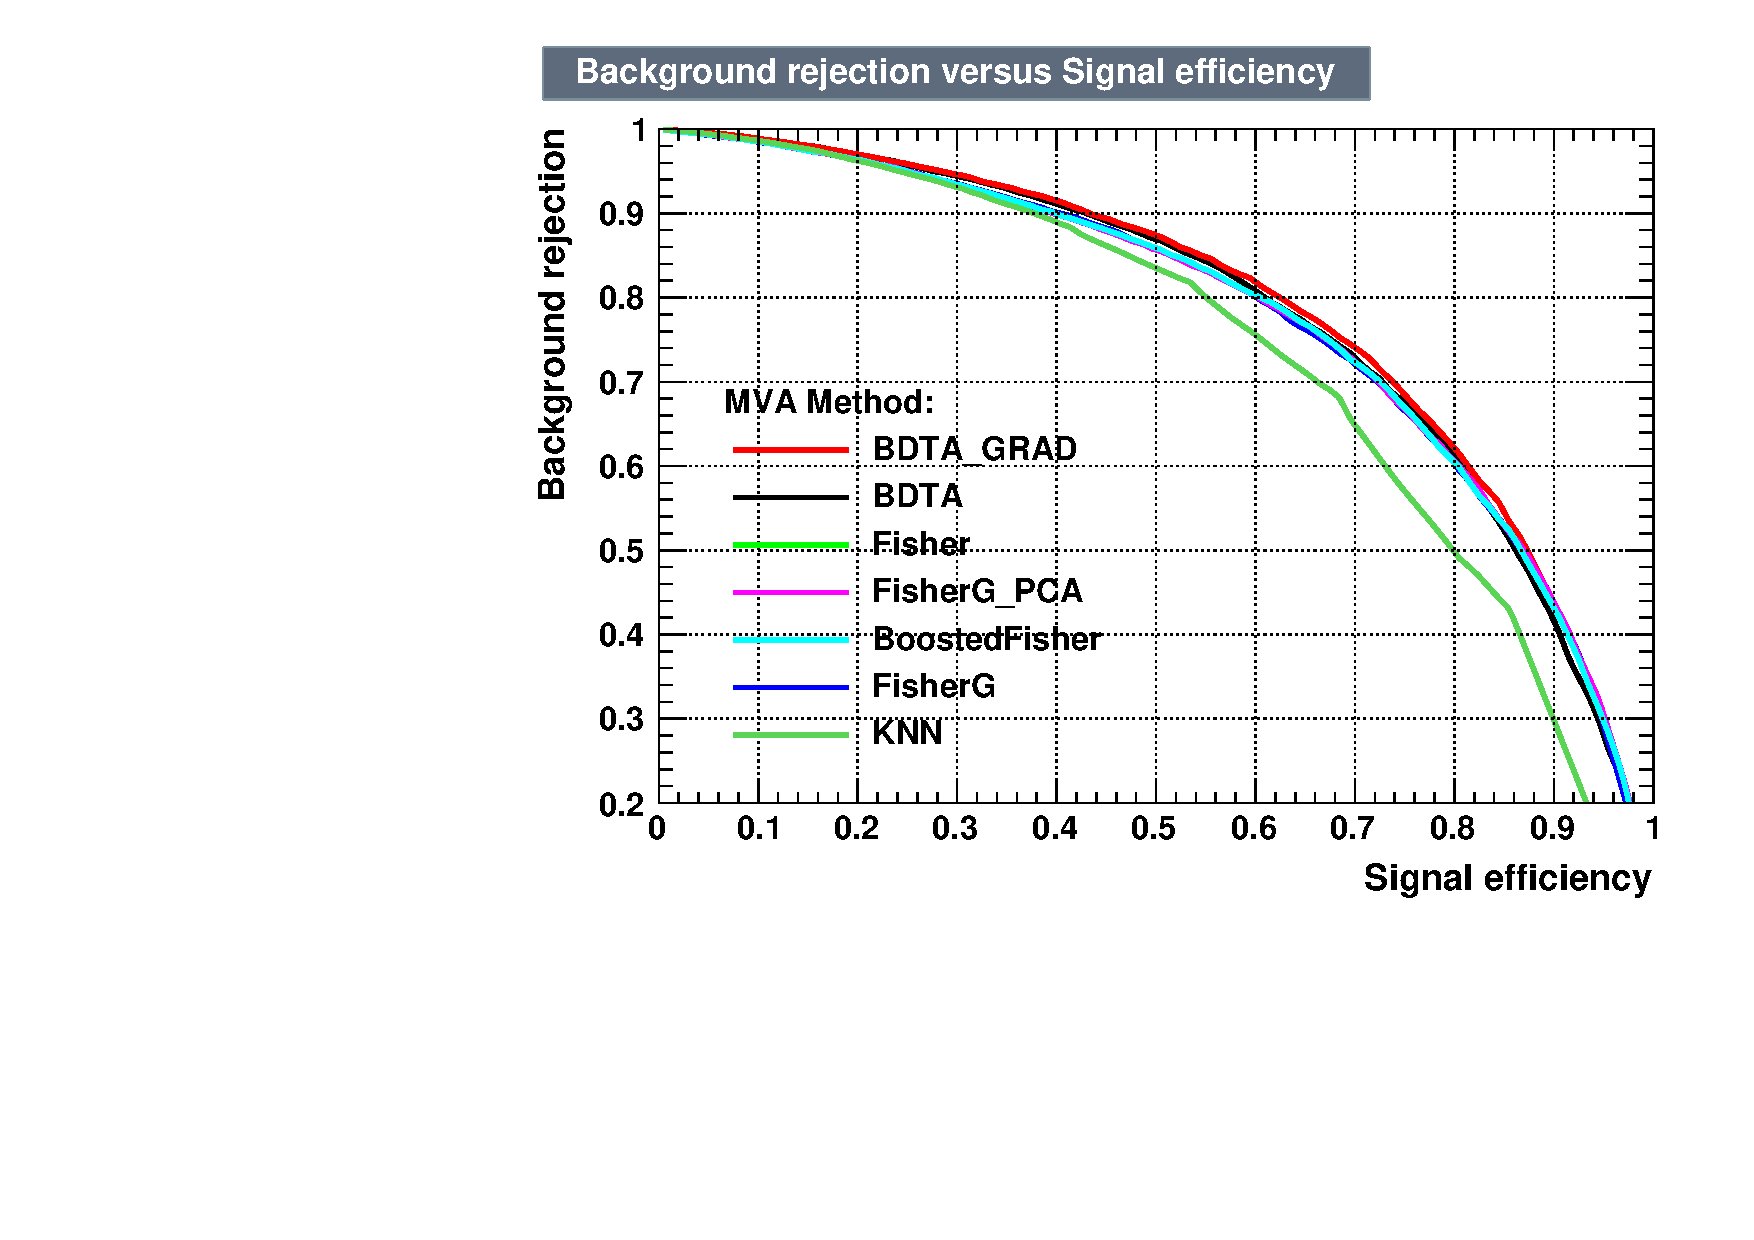
\includegraphics[width=0.4\textwidth]{figures/roc_ttv_3l_multimva.pdf}
   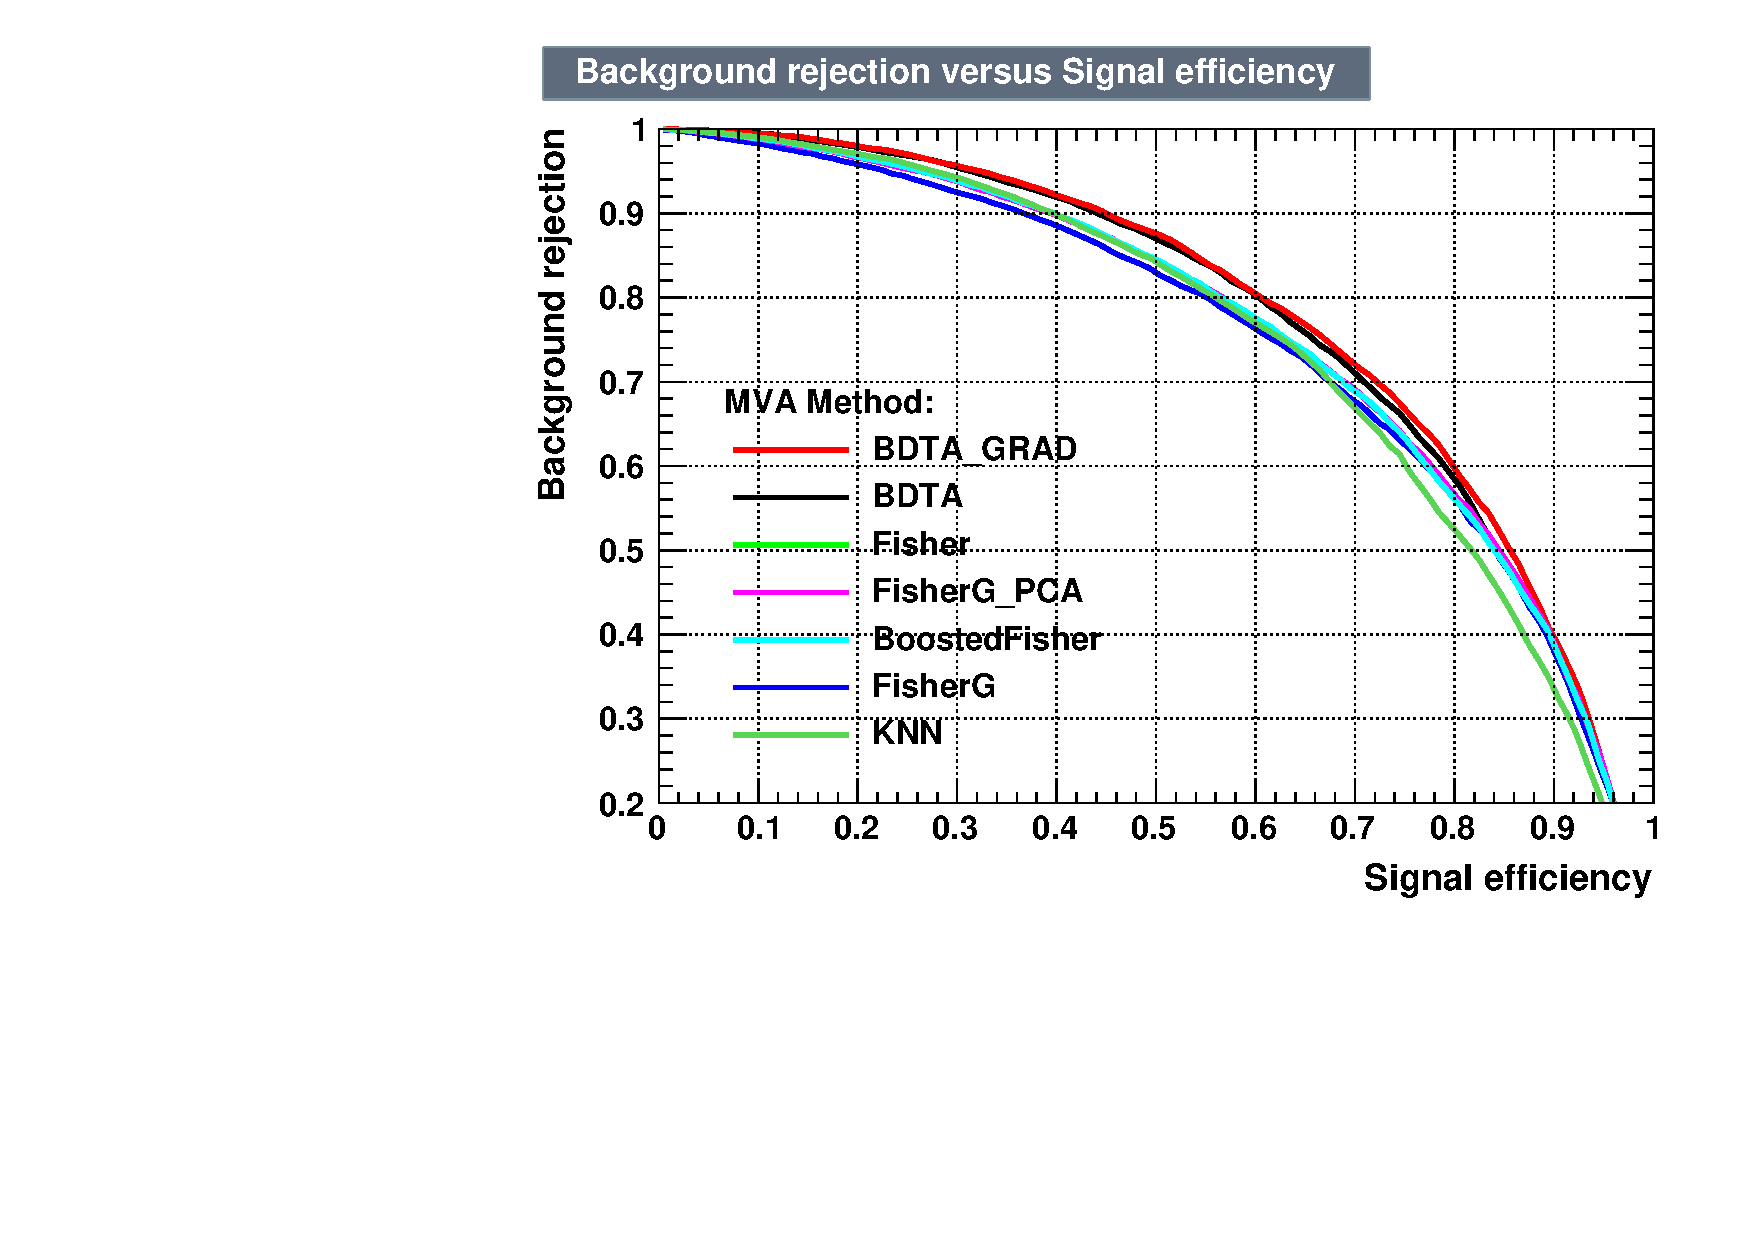
\includegraphics[width=0.4\textwidth]{figures/roc_tt_3l_multimva.pdf} \\
   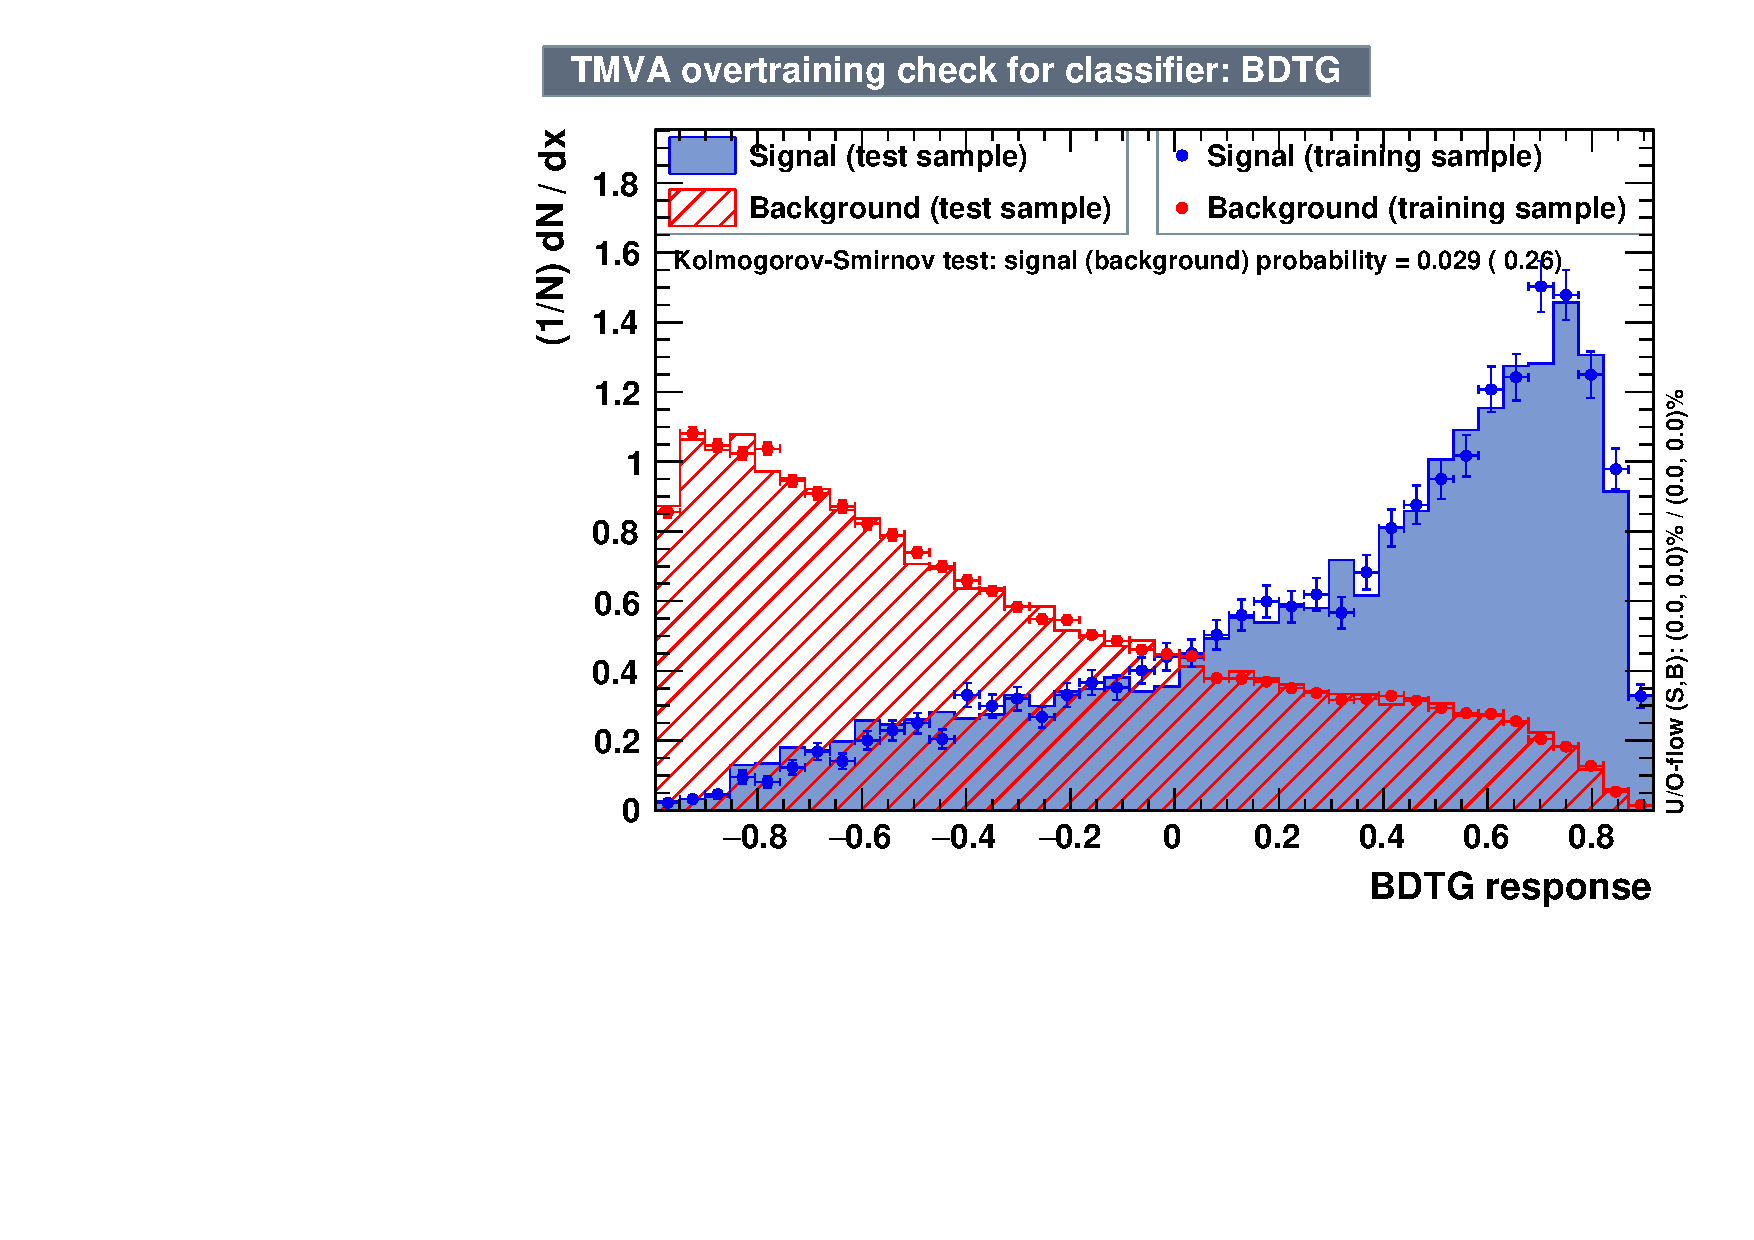
\includegraphics[width=0.4\textwidth]{figures/bdt_response_ttv_3l.pdf}
   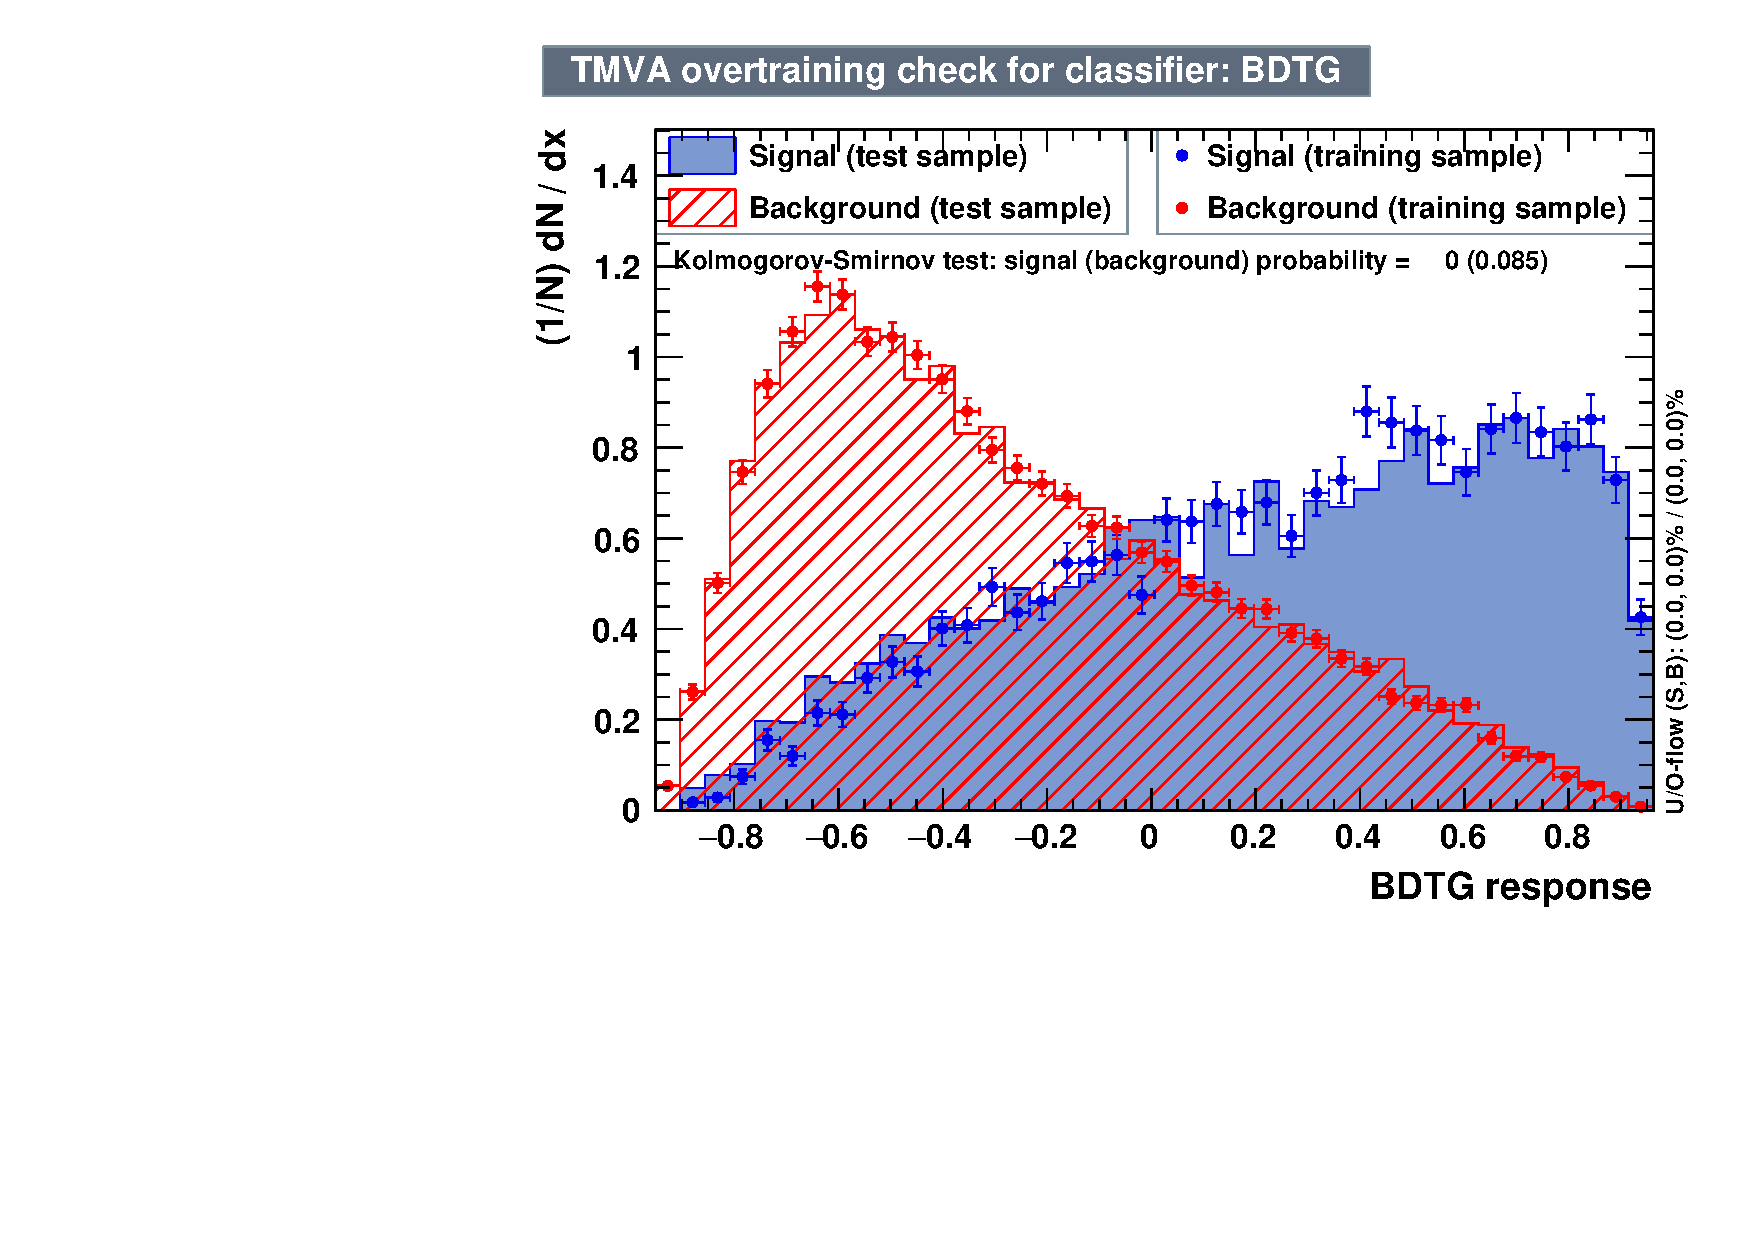
\includegraphics[width=0.4\textwidth]{figures/bdt_response_tt_3l.pdf}
\caption{Top: background rejection vs signal efficiency (ROC curves) for various MVA classifiers (top) in the three lepton channel against \ttV\ (left) and \ttbar\ (right). Bottom: classifier output distributions for the gradient boosted decision trees, for training against \ttV\ (left) and against \ttbar\ (right).}
\label{roc}
\end{figure} 

\begin{figure} [!h]
  \centering
   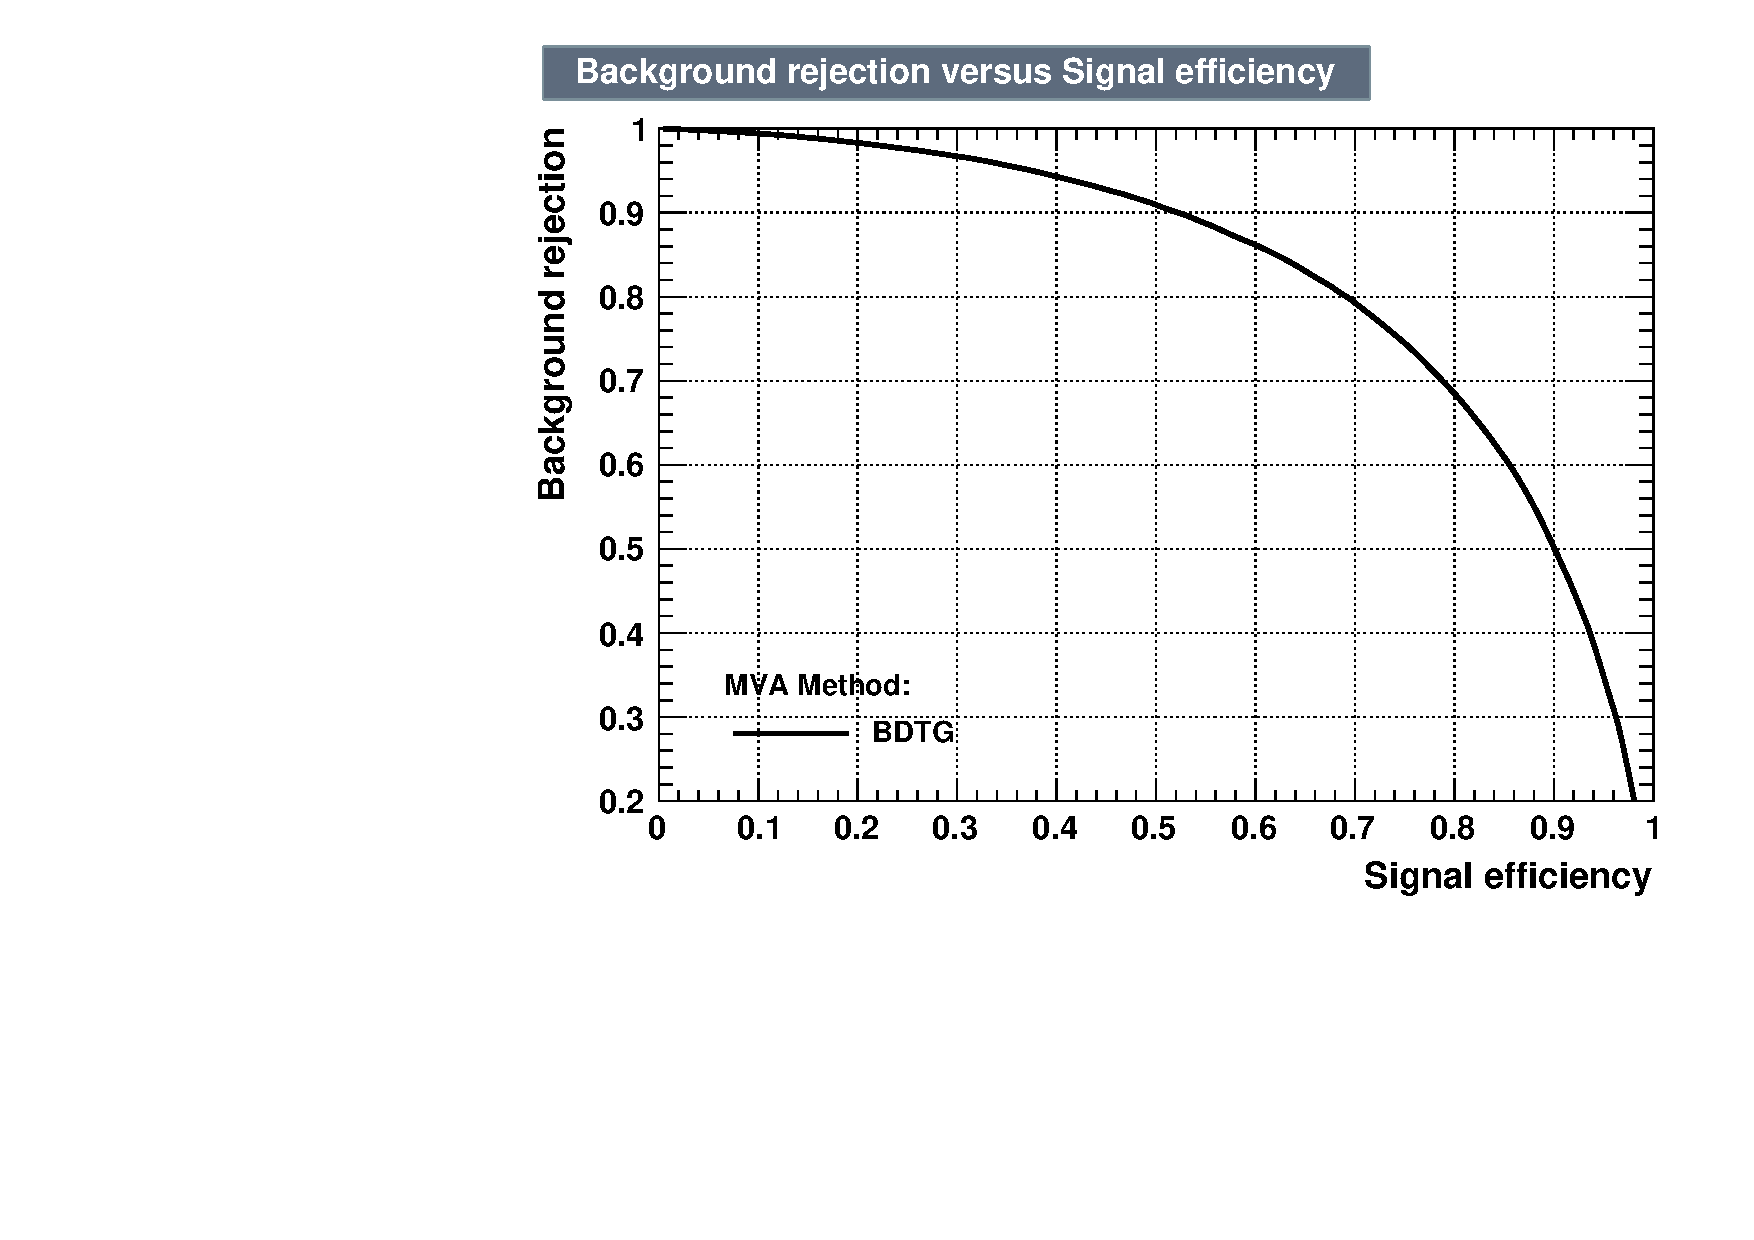
\includegraphics[width=0.4\textwidth]{figures/roc_ttv_2lss.pdf}
   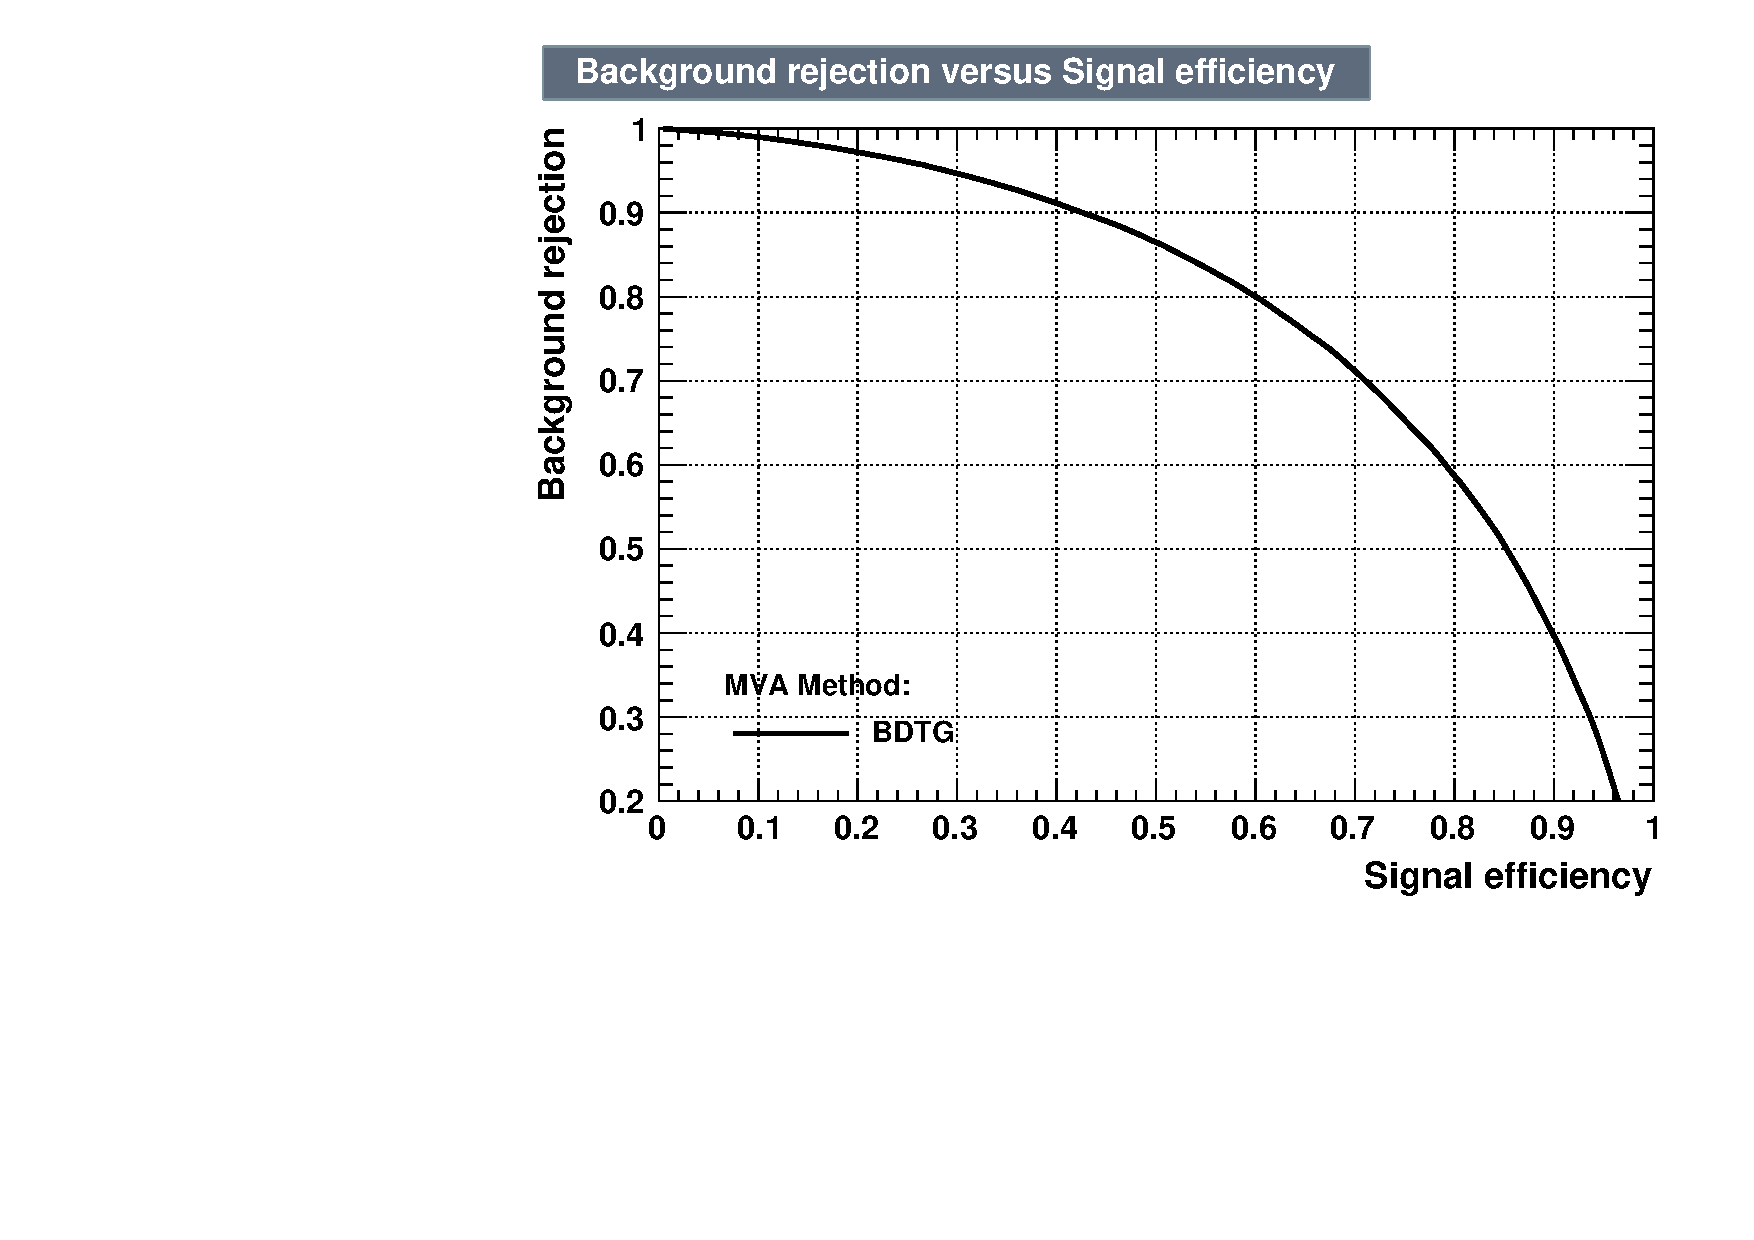
\includegraphics[width=0.4\textwidth]{figures/roc_tt_2lss.pdf} \\
   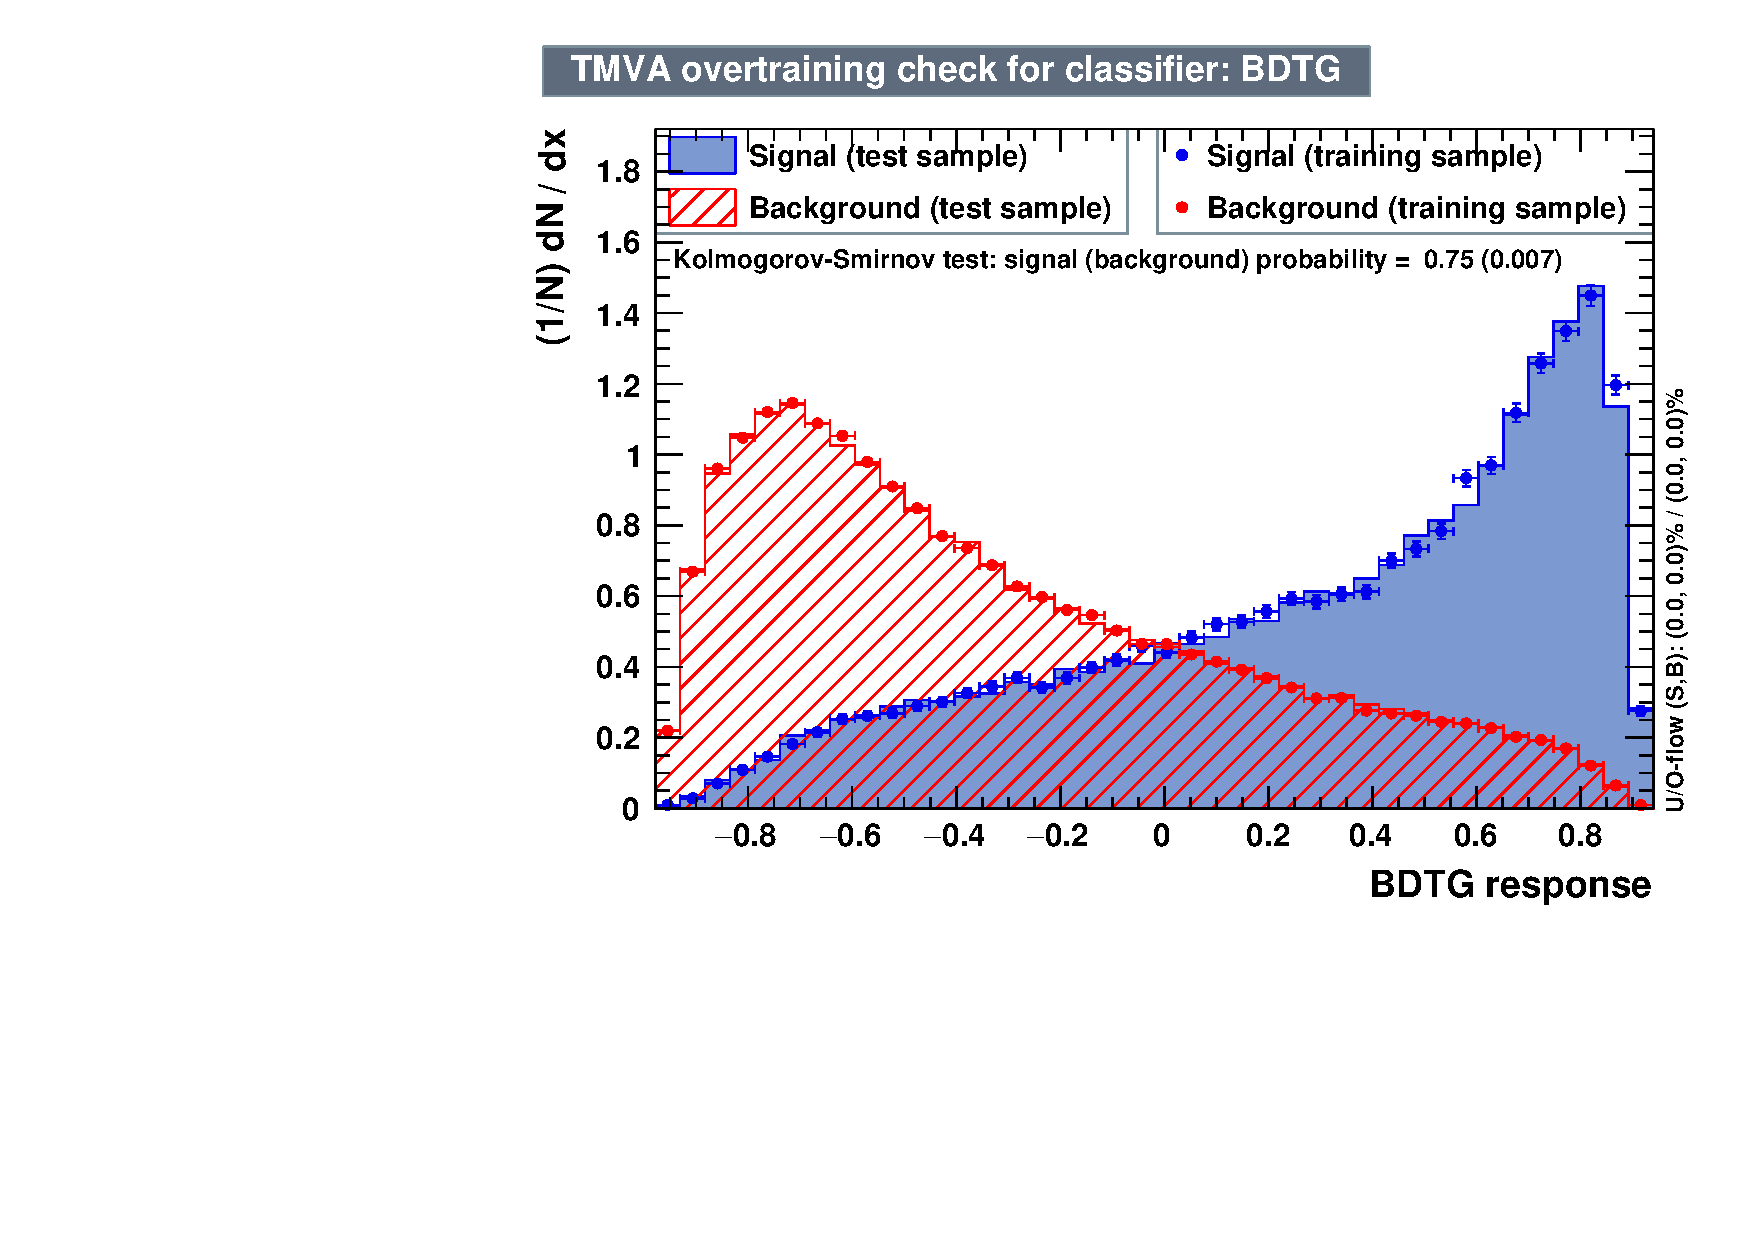
\includegraphics[width=0.4\textwidth]{figures/bdt_output_ttv_2lss.pdf}
   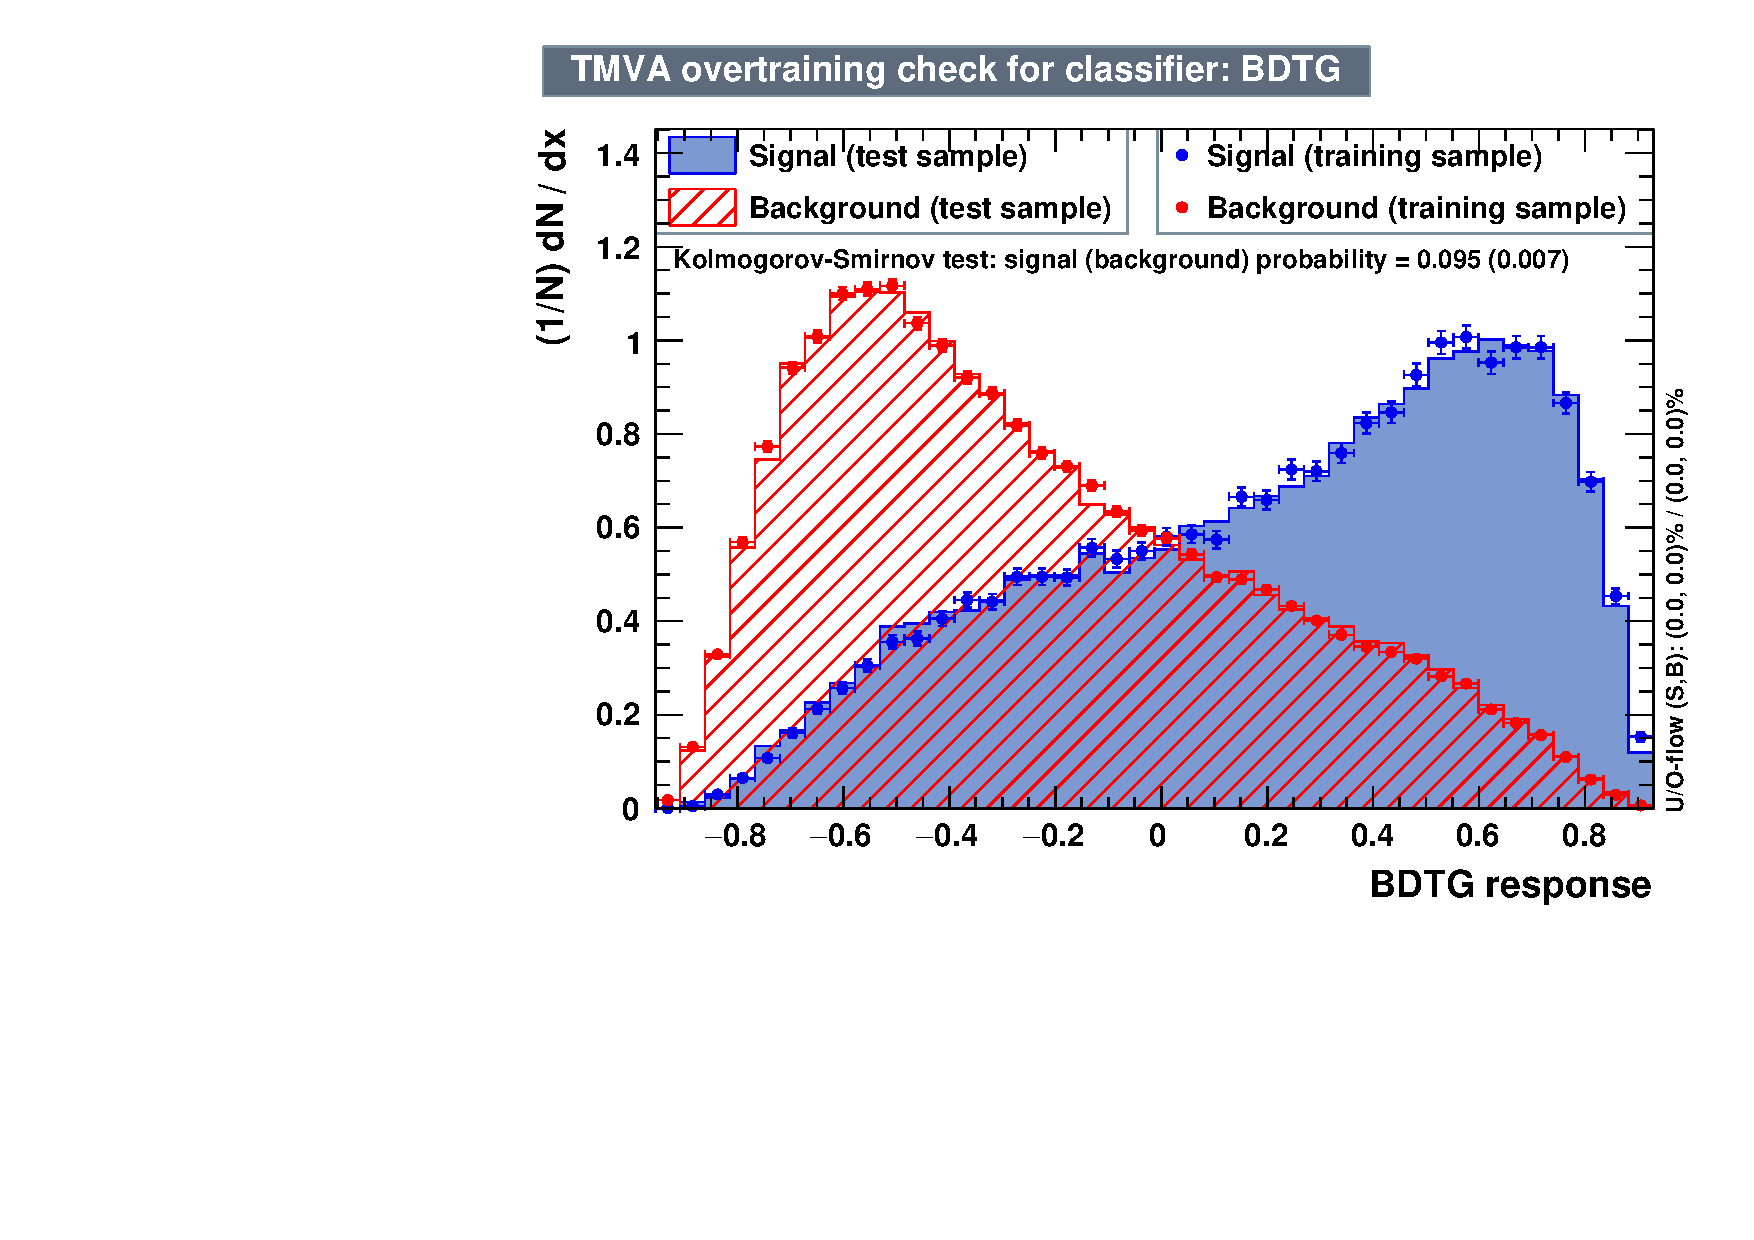
\includegraphics[width=0.4\textwidth]{figures/bdt_output_tt_2lss.pdf}
\caption{Top: background rejection vs signal efficiency (ROC curve) in the same sign dilepton channel for a single discriminator: BDTG, against \ttV\ (left) and \ttbar\ (right). Bottom: classifier output distribution, for training against \ttV\ (left) and against \ttbar\ (right).}
\label{output_2lss}
\end{figure}

In both cases the gradient boosted decision tree (``BDTA\_GRAD'') classifier offers the best results, followed by an adaptive BDT classifier (``BDTA''). 
The BDTA\_GRAD classifier output distributions for signal and backgrounds are shown on the bottom of Fig.~\ref{roc}.
As expected, a good discrimination power is obtained using default discriminator parameter values, with minimal overtraining.
TMVA provides a ranking of the input variables by their importance in the classification process, shown in Tab.~\ref{ranking}.

\begin{table}[h!]
\centering
\footnotesize
\begin{tabular}{lllll}
      &\multicolumn{2}{c}{ttbar training}             & \multicolumn{2}{c}{ttV training}\\\hline
Rank  & Variable             & Importance  & Variable             & Importance \\ \hline
    1 & minDRll              & 1.329e-01   & dEtaFwdJetBJet       & 1.264e-01\\
    2 & dEtaFwdJetClosestLep & 1.294e-01   & Lep3Pt               & 1.224e-01\\
    3 & dEtaFwdJetBJet       & 1.209e-01   & maxEtaJet25          & 1.221e-01\\
    4 & dPhiHighestPtSSPair  & 1.192e-01   & dEtaFwdJet2BJet      & 1.204e-01\\
    5 & Lep3Pt               & 1.158e-01   & dEtaFwdJetClosestLep & 1.177e-01\\
    6 & maxEtaJet25          & 1.121e-01   & minDRll              & 1.143e-01\\
    7 & dEtaFwdJet2BJet      & 9.363e-02   & dPhiHighestPtSSPair  & 9.777e-02\\
    8 & nJetEta1             & 6.730e-02   & nJet25\_Recl         & 9.034e-02\\
    9 & nJet25\_Recl         & 6.178e-02   & nJetEta1             & 4.749e-02\\
   10 & lepCharge            & 4.701e-02   & lepCharge            & 4.116e-02\\\hline

\end{tabular}
\caption{TMVA input variables ranking for BDTA\_GRAD method for the trainings in the three lepton channel. For both trainings the rankings show almost the same 5 variables in the first places.}

\label{ranking}
\end{table}

\begin{table}[h!]
\centering
\footnotesize
\begin{tabular}{lllll}
      &\multicolumn{2}{c}{ttbar training}             & \multicolumn{2}{c}{ttV training}\\\hline
Rank  & Variable             & Importance  & Variable             & Importance \\ \hline
    1 & dEtaFwdJetClosestLep & 1.394e-01   & maxEtaJet25          & 1.357e-01\\ 
    2 & minDRll              & 1.359e-01   & dEtaFwdJet2BJet      & 1.267e-01\\
    3 & maxEtaJet25          & 1.308e-01   & dEtaFwdJetBJet       & 1.200e-01\\
    4 & dPhiHighestPtSSPair  & 1.116e-01   & Lep2Pt               & 1.196e-01\\
    5 & Lep2Pt               & 1.111e-01   & dEtaFwdJetClosestLep & 1.145e-01\\
    6 & dEtaFwdJetBJet       & 1.067e-01   & minDRll              & 1.077e-01\\
    7 & dEtaFwdJet2BJet      & 8.906e-02   & nJet25\_Recl         & 1.020e-01\\
    8 & nJetEta1             & 6.445e-02   & dPhiHighestPtSSPair  & 8.232e-02\\
    9 & nJet25\_Recl         & 6.254e-02   & nJetEta1             & 5.948e-02\\
   10 & lepCharge            & 4.848e-02   & lepCharge            & 3.198e-02\\ \hline
\end{tabular}
\caption{TMVA input variables ranking for BDTA\_GRAD method in same-sign dilepton channel.}
\label{ranking}
\end{table}


The TMVA settings used in the BDT training are shown in Tab.~\ref{tab:bdtsettings}.

\begin{table}
\centering
\begin{tabular}{l}
  \hline
  \verb|TMVA.Types.kBDT| \\
  \verb|NTrees=800| \\
  \verb|BoostType=Grad| \\
  \verb|Shrinkage=0.10| \\
  \verb|!UseBaggedGrad| \\
  \verb|nCuts=50| \\
  \verb|MaxDepth=3| \\
  \verb|NegWeightTreatment=PairNegWeightsGlobal| \\
  \verb|CreateMVAPdfs| \\
  \hline
\end{tabular}
\caption{TMVA configuration used in the BDT training.}\label{tab:bdtsettings}
\end{table}


\section{Additional discriminating variables}

Two additional discriminating variables were tested considering the fact that the forward jet in the background could come from the pileup; since we have a real forward jet in the signal, it could give some improvement in the discriminating power. The additional variables describe the forward jet momentum (fwdJetPt25) and the forward jet identification(fwdJetPUID). Distributions for these variables in the three lepton channel are shown in the figure ~\ref{fwd_add_var_3l}. The forward jet identification distribution show that for both, signal and background, jets are mostly real jets. 

\begin{figure} [!h]
  \centering
   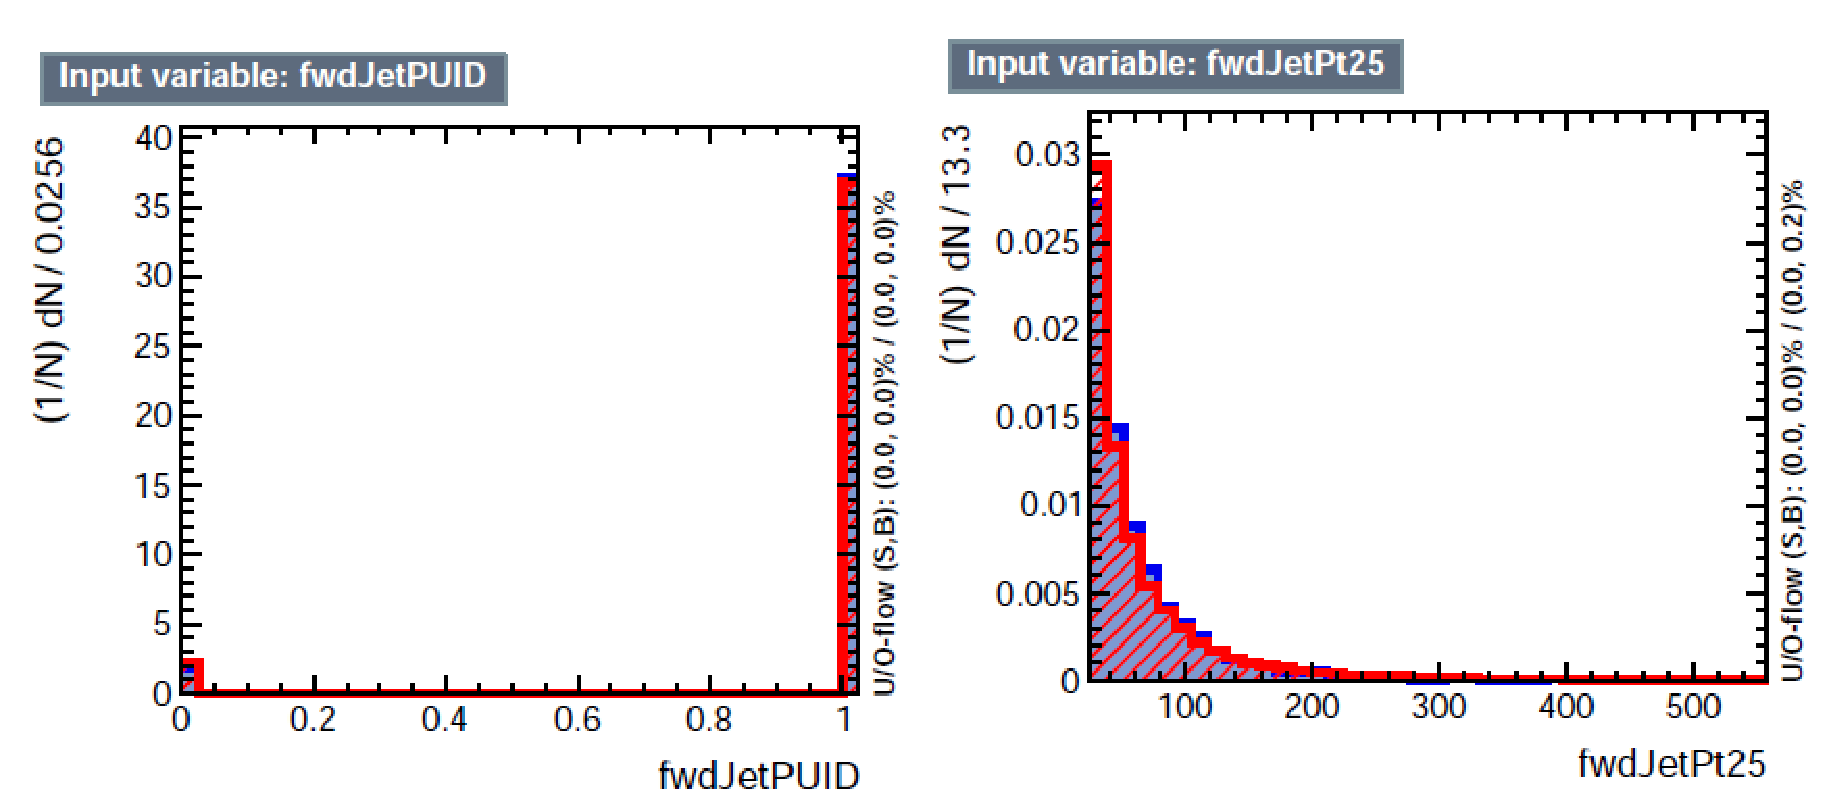
\includegraphics[width=0.9\textwidth]{figures/fwd_add_var_ttv_3l.pdf}\\
   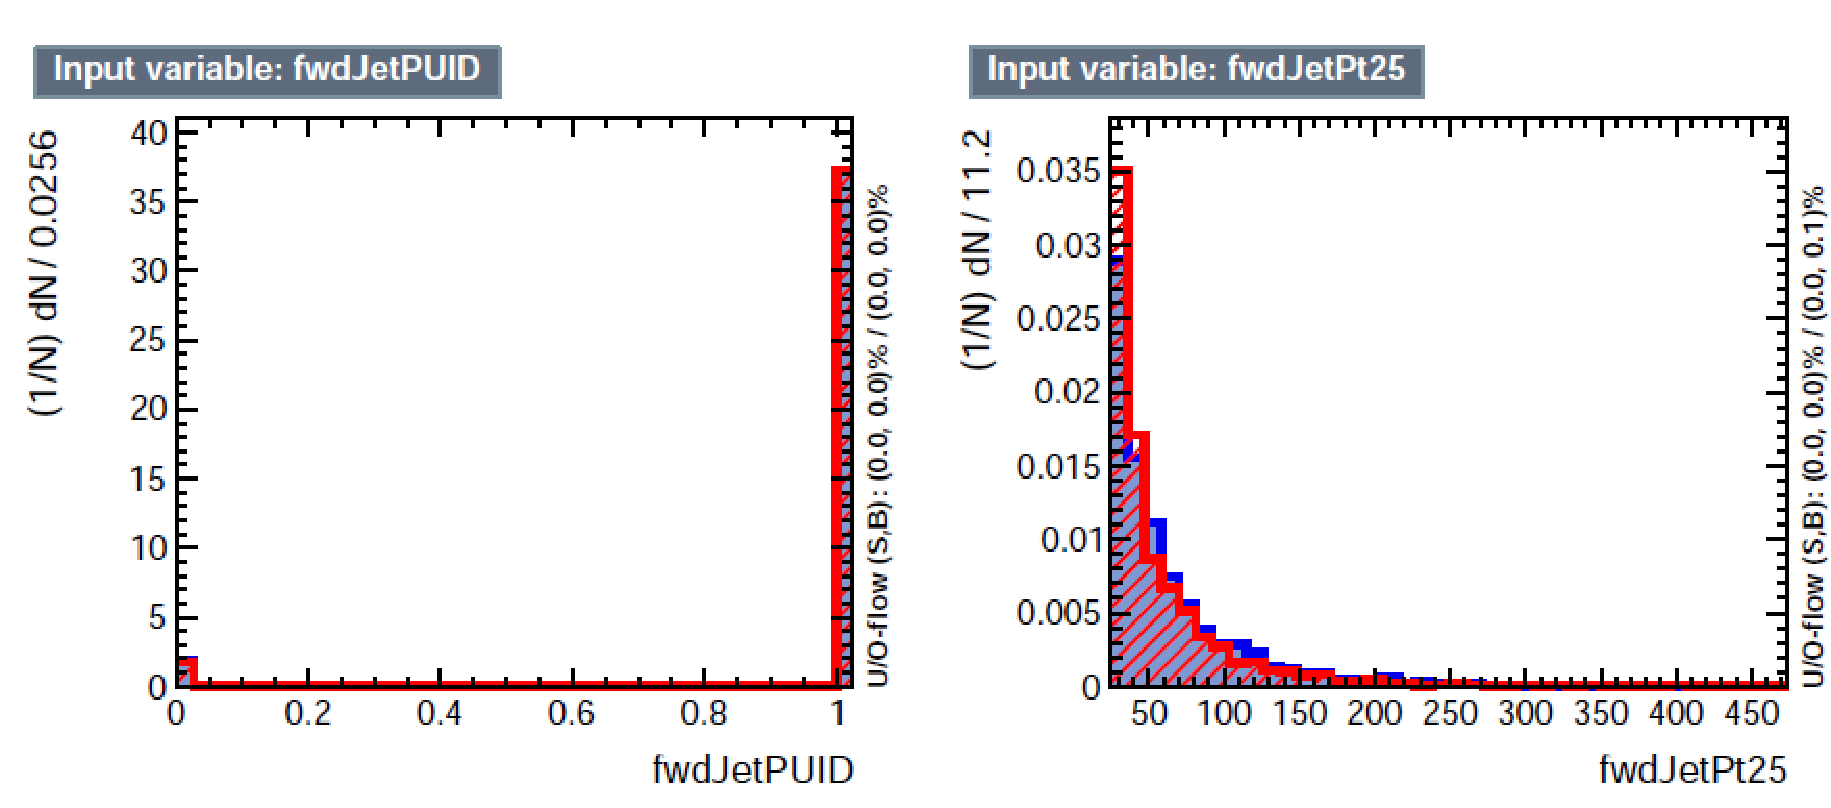
\includegraphics[width=0.9\textwidth]{figures/fwd_add_var_tt_3l.pdf}
\caption{Additional discriminating variables distributions for ttv training(Top row) and tt training (bottom row) in the three lepton channel. The origin of the jets in the forward jet identification distribution is tagged as 0 for ``pileup jets'' while ``real jets'' are tagged as 1.}
\label{fwd_add_var_3l}
\end{figure}

The testing was made including in the MVA input one variable at a time, so we can evaluate the dicrimination power of each variable, and then both simultaneously. fwdJetPUID was ranked in the last place in importance (11) in both training (ttV and tt) while fwdJetPt25 was ranked 3 in the ttV training and 7 in the tt training. When training using 12 variables, fwdJetPt25 was ranked 5 and 7 in the ttV and tt trainings respectively, while fwdJetPUID was ranked 12 in both cases.

The improvement in the discrimination performance provided by the additional variables is about 1\%, so we decided not to include them in the current procedure. Table ~\ref{tab:add_var_improvement} show the ROC-integral for all the testing cases we made.


\begin{table}
\centering
\begin{tabular}{lc}
  \hline
                 &  ROC-integral \\\hline               
base 10 var ttv  & 0.848\\
+ fwdJetPUID ttv & 0.849\\
+ fwdJetPt25 ttv & 0.856\\
12 var ttv       & 0.856\\\hline\hline
base 10 var tt   & 0.777\\
+ fwdJetPUID tt  & 0.777\\
+ fwdJetPt25 tt  & 0.787\\
12 var           & 0.787\\\hline

\end{tabular}
\caption{ROC-integral for all the testing cases we made in the evaluation of the additional variables discriminating power. The improvement in the discrimination performance provided by the additional variables is about 1\% }\label{tab:add_var_improvement}
\end{table}
